%! TEX root = guide.tex

% Possible arguments for the HKNdocument class:
% Language:
%   italian (default): Sets the document language to Italian.
%   english: Sets the document language to English.
%
% Table of Contents (ToC) depth:
%   toc=chapters: Shows only chapters in the ToC (tocdepth=0).
%   toc=sections: Shows chapters and sections in the ToC (tocdepth=1).
%   toc=subsections: Shows up to subsections in the ToC (default, tocdepth=2).
%   toc=subsubsections: Shows up to sub-subsections in the ToC (tocdepth=3).
%
% Font size:
%   10pt: Sets the base font size to 10 points.
%   11pt (default): Sets the base font size to 11 points.
%   12pt: Sets the base font size to 12 points.
%
% Draft mode:
%   draft: Compiles the document in draft mode (useful for proofreading, dummy images and imported files).
\documentclass[english,12pt,toc=sections]{HKNdocument}
% Packages
\usepackage{listings}                    % Code highlighting
\usepackage{xcolor}                      % Custom colors
\usepackage{longtable}                   % Breakable tables
\usepackage{ulem}                        % Underline
\usepackage{contour}                     % Border around text
\usepackage{tcolorbox}                   % Custom boxes

% Primary (Accent) Colors
% Primary (Accent) Colors
\definecolor{accentYellow}{RGB}{254, 196, 41}  % #FEC421
\definecolor{accentRed}{RGB}{236, 45, 36}      % #EC2D24

% Secondary Colors
\definecolor{supportOrange}{RGB}{242, 183, 5}  % #F2B705
\definecolor{supportDarkBlue}{RGB}{55, 81, 113} % #375171

% Background Colors
\definecolor{backgroundLight}{RGB}{242, 242, 242} % #F2F2F2

% Text & Border Colors
\definecolor{textGrayBlue}{RGB}{100, 117, 140}   % #64758C
\definecolor{textGrayMedium}{RGB}{146, 154, 166}  % #929AA6
\definecolor{textGrayLight}{RGB}{184, 187, 191}   % #B8BBBF



% Listings style
\lstdefinestyle{hkn}{
  basicstyle=\ttfamily\small\color{textGrayBlue},                         % Base style (size and font)
  keywordstyle=\bfseries\color{accentRed},           % Keywords in red (important, eye-catching)
  identifierstyle=\color{supportDarkBlue},               % Identifiers in blue (clear distinction)
  commentstyle=\color{textGrayMedium},                 % Comments in gray-blue (less prominent)
  stringstyle=\color{supportOrange},                 % Strings in orange (warm and readable)
  numberstyle=\ttfamily\scriptsize\color{textGrayMedium}, % Line numbers in gray (non-intrusive)
  backgroundcolor=\color{backgroundLight},           % Light background for contrast
  rulecolor=\color{textGrayLight},                   % Soft gray border for structure
  frame=single,                          % Border around code (single, double, shadowbox, none)
  framerule=0.8pt,                       % Border thickness
  frameround=tttt,                       % Round all corners
  framesep=5pt,                          % Distance between border and code
  rulesep=2pt,                           % Distance between border and code line
  numbers=left,                          % Line number position (left, right, none)
  stepnumber=1,                          % Line number interval
  numbersep=10pt,                        % Distance between line numbers and code
  xleftmargin=30pt,                      % Left margin
  xrightmargin=30pt,                     % Right margin
  resetmargins=true,                     % Reset margins
  numberblanklines=false,                % Number blank lines
  firstnumber=auto,                      % Initial line number
  columns=fixed,                         % Fixed column width
  showstringspaces=false,                % Show spaces in strings
  tabsize=2,                             % Tab size
  breaklines=true,                       % Automatic line break for long lines
  breakatwhitespace=true,                % Line break at whitespace
  breakautoindent=true,                  % Automatic indentation after line break
  escapeinside={(*@}{@*)}                % LaTeX commands in code
}

% Underline settings
\renewcommand{\ULdepth}{1.8pt} % Underline depth
\contourlength{0.8pt}

% Custom underline command
\newcommand{\myuline}[1]{%
\uline{\phantom{#1}}%
\llap{\contour{white}{#1}}%
}

% tcolorbox color settings
\definecolor{tcolorboxLeftColor}{RGB}{2, 65, 191}
\definecolor{tcolorboxBackTitleColor}{RGB}{119, 152, 255}
\definecolor{tcolorboxBackColor}{RGB}{210, 226, 255}

% Custom boxes
\newtcolorbox[auto counter, number within=chapter]{definition}[1]{
  title={\iflanguage{italian}{Definizione}{Definition}\par~\arabic{\tcbcounter}.~#1},
  boxrule=0mm,                       % Bordo principale (disabilitato)
  leftrule=1mm,                    % Bordo sinistro principale
  arc=2mm,
  colframe=accentRed,       % Colore bordo
  colbacktitle=textGrayMedium,
  colback=backgroundLight,        % Colore sfondo
  fonttitle=\bfseries,
  rounded corners=all,               % Bordi arrotondati
  }

\newtcolorbox[auto counter, number within=chapter]{theorem}[1]{
  title={\iflanguage{italian}{Teorema}{Theorem}~\arabic{\tcbcounter}.~#1},
  boxrule=0mm,                       % Bordo principale (disabilitato)
  leftrule=1mm,                    % Bordo sinistro principale
  arc=2mm,
  colframe=accentYellow,       % Colore bordo
  colbacktitle=textGrayMedium,
  colback=backgroundLight,        % Colore sfondo
  fonttitle=\bfseries,
  rounded corners=all,               % Bordi arrotondati
}

\newtcolorbox[auto counter, number within=chapter]{corollary}[1]{
  title={\iflanguage{italian}{Corollario}{Corollary}~\arabic{\tcbcounter}.~#1},
  boxrule=0mm,                       % Bordo principale (disabilitato)
  leftrule=1mm,                    % Bordo sinistro principale
  arc=2mm,
  colframe=supportOrange,       % Colore bordo
  colbacktitle=textGrayMedium,
  colback=backgroundLight,        % Colore sfondo
  fonttitle=\bfseries,
  rounded corners=all,               % Bordi arrotondati
}

\newtcolorbox[auto counter, number within=chapter]{exercise}[1]{
  title={\iflanguage{italian}{Esercizio}{Exercise}~\arabic{\tcbcounter}.~#1},
  boxrule=0mm,                       % Bordo principale (disabilitato)
  leftrule=1mm,                    % Bordo sinistro principale
  arc=2mm,
  colframe=supportDarkBlue,       % Colore bordo
  colbacktitle=textGrayMedium,
  colback=backgroundLight,        % Colore sfondo
  fonttitle=\bfseries,
  rounded corners=all,               % Bordi arrotondati
}

\newtcolorbox[auto counter, number within=chapter]{observation}[1]{
  title={\iflanguage{italian}{Osservazione}{Observation}~\arabic{\tcbcounter}.~#1},
  boxrule=0mm,                       % Bordo principale (disabilitato)
  leftrule=1mm,                    % Bordo sinistro principale
  arc=2mm,
  colframe=textGrayBlue,       % Colore bordo
  colbacktitle=textGrayMedium,
  colback=backgroundLight,        % Colore sfondo
  fonttitle=\bfseries,
  rounded corners=all,               % Bordi arrotondati
  }

\usepackage[english]{babel}
\usepackage{graphicx}
\usepackage{epstopdf}
\usepackage{xcolor}
\usepackage{titlesec}
\usepackage{mathtools}
\usepackage{booktabs}
\usepackage{array}
\usepackage{subfig}
\usepackage{tabularx}
\usepackage{float}
\usepackage{caption}
\usepackage{cancel}
\usepackage{lmodern}
\usepackage{amsmath}
\usepackage{amsfonts}
\usepackage{centernot}
\usepackage[super]{nth}
\counterwithin{equation}{section}
\counterwithin{figure}{section}
\newcommand{\diff}[1]{\mathrm{d}#1}
\newcommand{\dvec}[1]{\dot{\vec{#1}}}
\newcommand{\muz}{\mu_0}
\newcommand{\epsz}{\varepsilon_0}
\newcommand{\crossout}[1]{\cancel{#1}\raisebox{14pt}{\scriptsize = 0}}
\newcommand{\bigsum}{\displaystyle\sum}
\newcommand{\brackets}[1]{\left(#1\right)}
\newcommand{\dalambertref}{\hyperref[D'Alambert_principle]{D'Alambert's principle}}
\newcommand{\lagrangeref}{\hyperref[Lagrange_equations]{Lagrange equations}}
\newcommand{\eleref}{\hyperref[Euler_Lagrange_equations]{Euler-Lagrange equations}}
\newcommand{\hpquoteref}{\hyperref[q:Hamilton_principle_quote]{Hamilton's principle}}
\newcommand{\hpquotemath}{\hyperref[e:Hamilton_principle]{Hamilton's principle}}
\newcommand{\hamiltonref}{\hyperref[hamilton_equations]{Hamilton's equations}}
\newcommand{\defineeq}{\coloneqq}
\newcommand{\partialD}[2]{\dfrac{\partial #1}{\partial #2}}
\newcommand{\partialDD}[2]{\dfrac{\partial^2 #1}{\partial #2^2}}
\newcommand{\totalD}[2]{\dfrac{\diff{#1} }{\diff{#2}}}
\newcommand{\lagr}{\mathcal{L}}
\newcommand{\hamfun}{\mathcal{H}}
\newcommand{\efunction}{\mathrm{e}}
\newcommand{\pb}[2]{\left\{#1,#2\right\}}
\newcommand{\Velegant}{\mathcal{V}} %Aka V-sexy
\newcommand{\Telegant}{\mathcal{T}} %Aka T-sexy
\newcommand{\transpose}[1]{#1^{\;T}}
\newcommand{\notimplies}{\centernot\implies}


\begin{document}
% Document metadata
\title{Guide to conventions and packages for the HKNotes project}
\shorttitle{HKNotes Guide}
% You can include multiple \autor commands to list all autors in the frontpage.
\author{Mario Rossi}
\author{Luigi Bianchi}
\author{Anna Verdi}
\author{Giulia Neri}

% You can include multiple \editor commands to list all editors in the frontpage.
\editor{Paolo Gialli}
\editor{Sofia Blu}
\editor{Carlo Grigi}
\editor{Elisa Marroni}
\editor{Marco Violetti}

\organization{IEEE-HKN Mu Nu Chapter}
\docdate{\today}
\docversion{1.1}
\doclogo{hkn_logo_blu.png}
\doclicense{CC_BYNCND.png}

\frontmatter
% Create the title page
\maketitle

% Table of Contents after the title page
\clearpage
\cclicense
\clearpage
\tableofcontents
\clearpage

\mainmatter
\chapter{Introduction to analytical mechanics}
\section{One particle systems - Definitions}
For a single particle system of mass \textit{m}, which is moving along a trajectory we can define some properties:
\begin{itemize}
    \item Position: $\vec{r}$
    \item Velocity: $\vec{v} = \dfrac{\mathrm{d} \vec{r}}{\mathrm{d} t}=\dot{\vec{r}}$, which magnitude is called \textit{speed}
    \item Acceleration: $\vec{a}=\dfrac{\mathrm{d}^2 \vec{r}}{\mathrm{d} t^2}=\dot{\vec{v}}=\ddot{\vec{r}}$
\end{itemize}
\begin{figure}[H]
    \centering
    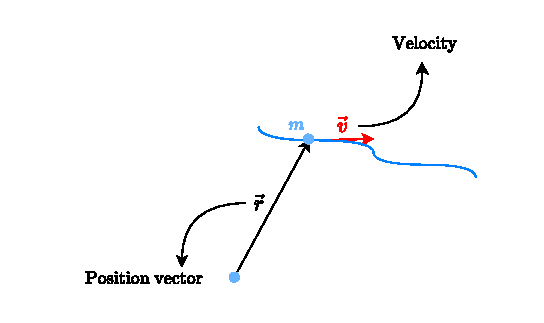
\includegraphics[width=0.6\textwidth]{res/svg/onepartsys.drawio}
    \caption{One particle system}
    \label{fig:image1}
\end{figure}

From that we can derive some quantities:
\begin{itemize}
    \item Linear momentum: \begin{equation}\vec{p}=m\vec{v}\end{equation} While $m$ is constant
    \item Total force applied: \begin{equation}\vec{F}=\dot{\vec{p}}=\dfrac{\mathrm{d} \vec{p}}{\mathrm{d} t}=m\vec{a}\end{equation}The first equality is the original formulation for Newton's second law.\\From this follows the conservation of linear momentum:
    \begin{equation}\vec{F}=0 \iff\dot{\vec{p}}=0 \iff\vec{p}\;\mathrm{is\;constant} \iff\vec{v}\;\mathrm{is\;constant}\end{equation}
    \item Angular momentum:
    \begin{equation}
        \vec{L_{\Omega}} = \left(\vec{r}-\vec{r}_{\Omega}\right) \wedge m\vec{v} = \left(\vec{r}-\vec{r}_{\Omega}\right) \wedge \vec{p}
    \end{equation}
    The angular momentum is a pseudo-vector and it is always calculated with reference to a generic point $\Omega$.
    \begin{figure}[H]
        \centering
        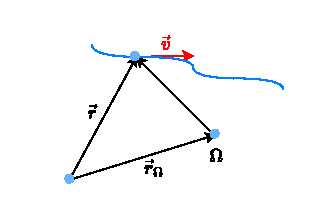
\includegraphics[width=0.6\textwidth]{res/svg/omegareference.drawio}
        \caption{Reference point for angular momentum}
        \label{fig:image2}
    \end{figure}
    Trying to differentiate the angular momentum we get:
    \begin{equation}
        \dfrac{\mathrm{d}\vec{L}_{\Omega}}{\mathrm{d}t} = \dfrac{\mathrm{d}}{\mathrm{d}t}\left(\left(\vec{r}-\vec{r}_{\Omega}\right) \wedge \vec{p}\right) = \dot{\vec{r}}\wedge\vec{p} - \dot{\vec{r}}_{\Omega}\wedge\vec{p} + \left(\vec{r}-\vec{r}_{\Omega}\right) \wedge \vec{F}
    \end{equation}
    \begin{equation}
        \dfrac{\mathrm{d}\vec{L}_{\Omega}}{\mathrm{d}t} = - \vec{v}_{\Omega}\wedge\vec{p} + \vec{\tau}_{\Omega}
    \end{equation}
    If $\Omega$ is at rest we can choose $\Omega = O$ which implies:
    \begin{equation}
        \dfrac{\mathrm{d}\vec{L}_{\Omega}}{\mathrm{d}t} = \vec{\tau}_{\Omega}
    \end{equation}
    From which follows the conservation of angular momentum:
    \begin{equation}
        \vec{\tau}_{\Omega} = 0 \iff\vec{L}_{\Omega}\;\mathrm{is\;constant}
    \end{equation}
    If $\vec{L}_{\Omega}$ is fixed then the trajectory happens on a plane.
    \begin{figure}[H]
        \centering
        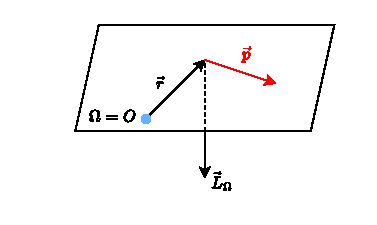
\includegraphics[width=0.6\textwidth]{res/svg/singleplanemotion.drawio}
        \caption{Motion on a single plane}
        \label{fig:image3}
    \end{figure}
\end{itemize}
\section{One particle systems - Work}
The work done by the total force on a particle from point $P_1$ to $P_2$ along a generic path can be visualized as:
\begin{figure}[H]
    \centering
    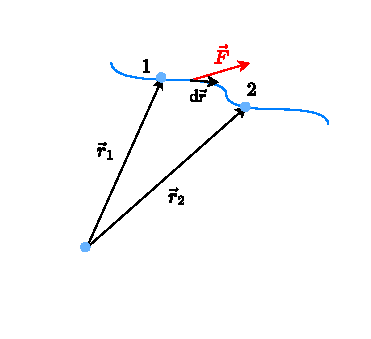
\includegraphics[width=0.5\textwidth]{res/svg/work.drawio}
    \caption{Work of the total force}
    \label{fig:image4}
\end{figure}
and is evaluated as:
\begin{equation}
    W_{12} = \int_{P_1}^{P_2}\vec{F}\cdot\mathrm{d}\vec{r} = \int_{P_1}^{P_2}\dfrac{\mathrm{d}}{\mathrm{d}t}(m\vec{v})\cdot\mathrm{d}\vec{r} = \int_{P_1}^{P_2}\dfrac{\mathrm{d}}{\mathrm{d}t}(m\vec{v})\cdot\vec{v}\mathrm{d}t =
\end{equation}
\begin{equation}
    = m\int_{P_1}^{P_2}\vec{v}\mathrm{d}v = \dfrac{1}{2}mv^2\bigg|_{P_1}^{P_2} = \dfrac{1}{2}mv_2^2 - \dfrac{1}{2}mv_1^2 = T_2 -T_1
\end{equation}
\begin{equation} \label{e:total_work}
    W_{12} = T_2 -T_1
\end{equation}
So the work done by the total force is the difference of the kinetic energy $T$ from point $P_1$ to $P_2$.\\
A force $\vec{f}$ is \textbf{conservative} if its work does not depend on the path:
\begin{equation}
    W_{12} = \int_{P_1,\gamma_1}^{P_2}\vec{f}\cdot\mathrm{d}\vec{r} = \int_{P_1,\gamma_2}^{P_2}\vec{f}\cdot\mathrm{d}\vec{r}\;\;\forall\;\gamma_1, \gamma_2
\end{equation}
\[\Updownarrow \]
\begin{equation}
    \int_{P_1,\gamma_1}^{P_2}\vec{f}\cdot\mathrm{d}\vec{r} - \int_{P_1,\gamma_2}^{P_2}\vec{f}\cdot\mathrm{d}\vec{r} = 0
\end{equation}
\begin{equation}
    \int_{P_1,\gamma_1}^{P_2}\vec{f}\cdot\mathrm{d}\vec{r} + \int_{P_2,\gamma_2}^{P_1}\vec{f}\cdot\mathrm{d}\vec{r} = 0
\end{equation}
\begin{equation}
    \oint\vec{f}\cdot\mathrm{d}\vec{r} = 0
\end{equation}
So if a force is conservative then its circulation is always 0 for any closed path.\\
Also if $\vec{f}$ is conservative we can find a scalar function such that:
\begin{equation}
    \int_{P_1,\gamma}^{P_2}\vec{f}\cdot\mathrm{d}\vec{r} = V_1-V_2
\end{equation}
This function is called the \textbf{potential}:
\begin{equation}
    V_1-V_2 = \int_{P_1}^{P_2}(-\mathrm{d}V) \Rightarrow \vec{f}\cdot\mathrm{d}\vec{r} = -\mathrm{d}V = -\nabla V \cdot \mathrm{d}\vec{r}
\end{equation}
\begin{equation}
    \vec{f} = -\nabla V
\end{equation}
If the total force $\vec{F}$ is conservative (sum of conservative forces) then:
\begin{equation}
    \vec{F} = \bigsum_{i=1}^{N} \vec{f}_i
\end{equation}
\begin{equation}
    W_{12}=\int_{P_1}^{P_2}\vec{f}\cdot\mathrm{d}\vec{r} = \int_{P_1,\gamma}^{P_2}-\nabla V\cdot\mathrm{d}\vec{r}
\end{equation}
Where $V$ is the sum of the potential of the single forces. Now from \eqref{e:total_work}, for conservative forces we get:
\begin{equation} \label{e:mech_energy}
    T_2 - T_1 = V_1 - V_2 \iff T_1 + V_1 = T_2 + V_2\iff E_1 = E_2
\end{equation}
Where $E$ is the total \textbf{mechanical energy} of the system.\\
There can be cases such that:
\begin{equation}
    \vec{F} = -\nabla V \;\;\;\mathrm{but}\;V=V(\vec{r},t)
\end{equation}
then $\vec{F}$ cannot be conservative. We can show this by computing $\mathrm{d}V$:
\begin{equation}
    -\mathrm{d}V = -\left(\dfrac{\partial V}{\partial x}\mathrm{d}x + \dfrac{\partial V}{\partial y}\mathrm{d}y + \dfrac{\partial V}{\partial z}\mathrm{d}z + \dfrac{\partial V}{\partial t}\mathrm{d}t\right) =
\end{equation}
\begin{equation}
    = -\nabla V \cdot\mathrm{d}\vec{r} - \dfrac{\partial V}{\partial t}\mathrm{d}t \neq \vec{F}\cdot\mathrm{d}\vec{r} \Rightarrow \int_{P_1}^{P_2}\vec{F}\cdot\mathrm{d}\vec{r} \neq V_1-V_2
\end{equation}
\section{Multiple particles systems - Definitions}
Similarly to what we established for one particle systems we can define some main characteristics for multiple particles systems:
\begin{itemize}
    \item Mass:\begin{equation}
        M = \bigsum_{i=1}^{N} m_i
    \end{equation}
    \item Linear momentum:\begin{equation}
        \vec{P} = \bigsum_{i=1}^{N} \vec{p}_i
    \end{equation}
    \item Angular momentum (with respect to $\Omega$):\begin{equation}
        \vec{L}_{\Omega} = \bigsum_{i=1}^{N} \left(\left(\vec{r}_i-\vec{r}_{\Omega}\right) \wedge \vec{p}_i\right)
    \end{equation}
    \item Average position (centre of mass): \begin{equation} \label{e:centre_of_mass}
        \vec{R} = \dfrac{\bigsum_{i=1}^{N}m_i\vec{r}_i}{\bigsum_{i=1}^{N}m_i}
    \end{equation}
    From this trivially follows:
    \begin{equation}
        M \vec{R} = \bigsum_{i=1}^{N}m_i\vec{r}_i
    \end{equation}
    \begin{equation}
        \dfrac{\mathrm{d}}{\mathrm{d}t}(M \vec{R}) = \dfrac{\mathrm{d}}{\mathrm{d}t}\left(\bigsum_{i=1}^{N}m_i\vec{r}_i\right)
    \end{equation}
    \begin{equation}
        M \dot{\vec{R}} = \vec{P}
    \end{equation}
    Where $\vec{v}_{CM} = \dot{\vec{R}}$ is the velocity of the centre of mass.
\end{itemize}
\section{Multiple particles systems - Newton's third law}
The total force on a single particle contains two components:
\begin{itemize}
    \item internal forces
    \item external forces
\end{itemize}
\begin{equation}
    \vec{F}_i = \vec{F}_i^{(\mathrm{ext})} + \bigsum_{i\neq j}^{N}\vec{F}_{ji}
\end{equation}
We will restrict to the case where $\vec{F}_{ji} = -\vec{F}_{ij}$. This is called \textbf{weak action law}, since it only requires that the forces are equal and opposite, but it is not necessary that they both lie on the same line.\\
\textbf{Newton's third law} (strong action law) is not always true. Let's show a counterexample.\\
Let there be two charges $q_1,q_2$ with velocity $v_1,v_2$ such that $v_1\perp v_2$. Analysing the moment when particle 2 is on the same line of motion of particle 1, for electrostatic forces we get:
\[||\vec{r}_{12}|| = ||\vec{r}_{21}|| = r\]
\[\vec{r}_{12} = - \vec{r}_{21}\]
\begin{equation}
    \vec{F}_{12} = k\dfrac{q_1q_2}{r^2}\hat{u}_{12} = k\dfrac{q_1q_2 \vec{r}_{12}}{r^3}
\end{equation}
\begin{equation}
    \vec{F}_{21} = k\dfrac{q_1q_2}{r^2}\hat{u}_{21} = k\dfrac{q_1q_2 \vec{r}_{21}}{r^3}
\end{equation}
So these forces satisfy both action laws, but these are not the only forces on the charges. Let's analyze the Lorentz's forces. Particle 1 feels a magnetic field:
\begin{equation}
    \vec{B}_{21} = \dfrac{\muz}{4\pi}\dfrac{q_2\vec{v}_2\wedge\vec{r}_{21}}{r} \neq 0
\end{equation}
Instead particle 2 does not feel any magnetic field since in the chosen moment it is in the direction of motion of the other charge so we have:
\begin{equation}
    \vec{B}_{12} = \dfrac{\muz}{4\pi}\dfrac{q_1\vec{v}_1\wedge\vec{r}_{12}}{r} = 0
\end{equation}
This means that the Lorentz's forces are:
\begin{equation}
    \vec{F}_{21} = q_1\vec{v}_1\wedge\vec{B}_{21} \neq 0
\end{equation}
\begin{equation}
    \vec{F}_{12} = q_2\vec{v}_2\wedge\vec{B}_{12} = 0
\end{equation}
Hence $\vec{F}_{21} \neq \vec{F}_{12}$ and Newton's thrid law is not satisfied.\\
Since we restrict our cases we have:
\begin{equation}
    \vec{F} = \bigsum_{i=1}\vec{F}_i = \bigsum_{i=1}\vec{F}_i^{\;(ext)} + \cancel{\bigsum_{i=1}\bigsum_{j\neq i}\vec{F}_i}\raisebox{14pt}{\scriptsize = 0}
\end{equation}
\begin{equation}
    \vec{F} = \bigsum_{i=1}\vec{F}_i = \bigsum_{i=1}\dfrac{\dd{\vec{p}_i}}{\dd{t}} = \dfrac{\dd{}}{\dd{t}}\bigsum_{i=1}\vec{p}_i = \dfrac{\dd{\vec{P}}}{\dd{t}}
\end{equation}
But also:
\begin{equation}
    \dfrac{\dd{\vec{P}}}{\dd{t}} = \bigsum_{i=1}\vec{F}_i^{\;(ext)}
\end{equation}
So (only if weak action law holds):
\begin{equation}
    \vec{F} = \dfrac{\dd{\vec{P}}}{\dd{t}}
\end{equation}
\section{Multiple particles systems - Angular momentum}
Starting from the definition:
\begin{equation}
    \vec{L}_{\Omega} = \bigsum_{i}\brackets{\vec{r}_i-\vec{r}_{\Omega}}\wedge\vec{p}_i
\end{equation}
\begin{equation}
    \dfrac{\dd{\vec{L}_{\Omega}}}{\dd{t}} = \bigsum_{i}\dfrac{\dd{}}{\dd{t}}\brackets{\vec{r}_i-\vec{r}_{\Omega}}\wedge\vec{p}_i + \bigsum_{i}\brackets{\vec{r}_i-\vec{r}_{\Omega}}\wedge\dfrac{\dd{\vec{p}_i}}{\dd{t}} =
\end{equation}
\begin{equation}
    = \crossout{\bigsum_{i}\vec{v}_i\wedge\vec{p}_i}-\bigsum_{i}\vec{v}_{\Omega}\wedge\vec{p}_i + \bigsum_{i}\brackets{\vec{r}_i-\vec{r}_{\Omega}}\wedge\vec{F}_i =
\end{equation}
\begin{equation}
    = -\vec{v}_{\Omega}\wedge\bigsum_{i}\vec{p}_i + \bigsum_{i}\brackets{\vec{r}_i-\vec{r}_{\Omega}}\wedge\vec{F}_i = -\vec{v}_{\Omega}\wedge\vec{P} + \bigsum_{i}\brackets{\vec{r}_i-\vec{r}_{\Omega}}\wedge\vec{F}_i
\end{equation}
We can simplify the first term since $\vec{v}_i \parallel \vec{p}_i$ and we can also see that the last term is the \textbf{total torque} $\vec{\tau}_{\Omega}$, which is the result of both the internal and external forces.
\begin{equation} \label{e:first_angular_expression}
    \dfrac{\dd{\vec{L}_{\Omega}}}{\dd{t}} = -\vec{v}_{\Omega}\wedge\vec{P} + \vec{\tau}_{\Omega}
\end{equation}
If we restrict to the strong action law we get:
\begin{equation}
    \vec{\tau}_{\Omega} = \bigsum_{i}\brackets{\vec{r}_i-\vec{r}_{\Omega}}\wedge\vec{F}_i = \bigsum_{i}\brackets{\vec{r}_i-\vec{r}_{\Omega}}\wedge\brackets{\vec{F}_i^{\;(ext)}+ \bigsum_{i\neq j}\vec{F}_{ji}} =
\end{equation}
\begin{equation}
    = \bigsum_{i}\brackets{\vec{r}_i-\vec{r}_{\Omega}}\wedge\vec{F}_i^{\;(ext)} + \crossout{\bigsum_{i}\brackets{\brackets{\vec{r}_i-\vec{r}_{\Omega}}\wedge\bigsum_{i\neq j}\vec{F}_{ji}}} = \vec{\tau}^{\;(ext)}
\end{equation}
We can cross out the second term since the sum only has terms such as:
\begin{equation}
    \vec{r}_i\wedge\vec{F}_{ji} + \vec{r}_j\wedge\vec{F}_{ij}-\crossout{{\vec{r}_{\Omega}\wedge\vec{F}_{ij}+\vec{r}_{\Omega}\wedge\vec{F}_{ji}}}
\end{equation}
This first simplification is a trivial consequence of weak action law. In order to simplify the other term we can realize that if strong action law holds then both $\vec{F}_{ij}$ and $\vec{F}_{ji}$ lie on the line of $\vec{r}_i-\vec{r}_j$ and have opposite directions.
So we get:
\begin{equation}
    \bigsum_{i}\brackets{\brackets{\vec{r}_i-\vec{r}_{\Omega}}\wedge\bigsum_{i\neq j}\vec{F}_{ji}} = 0
\end{equation}
Going back to \eqref{e:first_angular_expression} we get:
\begin{equation}
    \dfrac{\dd{\vec{L}_{\Omega}}}{\dd{t}} = -\vec{v}_{\Omega}\wedge\vec{P} + \vec{\tau}^{\;(ext)}
\end{equation}
The first term can be 0 if:
\begin{itemize}
    \item $\Omega$ is at rest
    \item $\Omega$ is a point such that $\vec{v}_{\Omega} \parallel \vec{P}$ (for example the centre of mass)
    \item $\vec{P}=0$
\end{itemize}
So in the case of $\Omega = \mathrm{CM}$ we have:
\begin{equation} \label{e:first_cardinal}
    \dfrac{\dd{\vec{L}_{\Omega}}}{\dd{t}} = \vec{\tau}_{\Omega}
\end{equation}
Then:
\begin{equation}
    \vec{L}_{\Omega}\;\mathrm{is\;constant} \iff \vec{\tau}_{\Omega}^{\;(ext)}=0
\end{equation}
The centre of mass also satisfies:
\begin{equation}
    \vec{P} = M\dvec{R}
\end{equation}
as if the mass was all concentrated in the CM. But for angular momentum:
\begin{equation}
    \vec{L}_{\Omega} \neq (\vec{R}-\vec{r}_{\Omega})\wedge\vec{P}
\end{equation}
instead this is true:
\begin{equation}
    \vec{L}_{\Omega} = (\vec{R}-\vec{r}_{\Omega})\wedge\vec{P} + \vec{L}'_{CM}
\end{equation}
Where $\vec{L}'_{CM}$ is the total angular momentum evaluated in the frame of reference of the centre of mass.\\
From this we can state \textbf{Konig's theorem}:
\begin{equation}
    T = \dfrac{1}{2}\bigsum_i m_i v_i^2 = T_{CM} + T' = \dfrac{1}{2}M v_{CM}^2 + T'
\end{equation}
Where $T'$ is the kinetic energy associated to the motion with respect to the centre of mass.\\
Now we can analyze the work of the system of particles:
\begin{equation}
    W_{12} = \bigsum_i\int_{1}^{2}\vec{F}_i = \int_{1}^{2}\bigsum_i\vec{F}_i = \int_{1}^{2}\bigsum_i\brackets{\vec{F}_i^{\;(ext)} + \bigsum_{j\neq i}\vec{F}_{ji}}\cdot \dd{\vec{r}_i} =
\end{equation}
\begin{equation}
    = \int_{1}^{2}\brackets{\bigsum_i\vec{F}_i^{\;(ext)} + \bigsum_i\bigsum_{j\neq i}\vec{F}_{ji}}\cdot \dd{\vec{r}_i}
\end{equation}
The term $\bigsum_i\bigsum_{j\neq i}\vec{F}_{ji}\cdot \dd{\vec{r}_i}$ is not necessarily 0, but it is 0 in the case of rigid bodies.\\
If external forces are conservative:
\begin{equation}
    \vec{F}_i^{\;(ext)} = -\nabla_i V_i
\end{equation}
The gradient with respect to i is $\nabla_i = \brackets{\partial_{x_i}, \partial_{y_i}, \partial_{z_i}}$. So the work of external forces is just:
\begin{equation}
    W_{12}^{\;(ext)} = \int_{1}^{2}\bigsum_i\brackets{\vec{F}_i\cdot\dd{\vec{r}_i}} = -\bigsum_i\int_{1}^{2}\nabla_i V_i\cdot\dd{\vec{r}_i} =
\end{equation}
\begin{equation}
    = -\bigsum_i\int_{1}^{2}\dd{V_i} = -\bigsum_i V_i\bigg|_1^2
\end{equation}
Now defining $V^{\;(ext)} = \bigsum_i V_i$ we get:
\begin{equation}
    W_{12}^{\;(ext)} = V^{\;(ext)}_1 - V^{\;(ext)}_2
\end{equation}
Now we can see that if forces obey both the strong and the weak action law both $\vec{F}_{ji}$ and $\vec{F}_{ij}$ lie on the line of $\vec{r}_{ij} = \vec{r}_i-\vec{r}_j$ as shown in this example:
\begin{figure}[H]
    \centering
    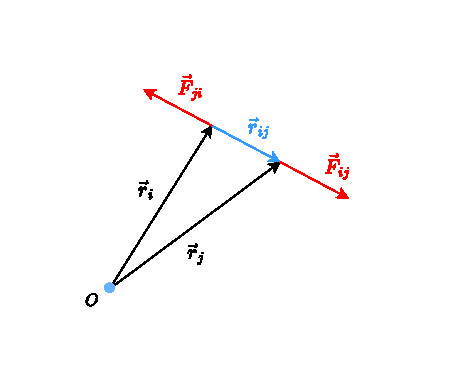
\includegraphics[width=0.5\textwidth]{res/svg/forcesstronglaw.drawio}
    \caption{Forces with strong action law}
    \label{fig:image5}
\end{figure}
Now assuming the forces are conservative we can express them as:
\begin{itemize}
    \item $\vec{F}_{ij}= -\nabla_{j}V_{ij}$
    \item $\vec{F}_{ji}= -\nabla_{i}V_{ji}$
\end{itemize}
But in this case $V_{ij}=V_{ji}$ so, from the strong action law we get:
\begin{equation}
    -\nabla_iV_{ij}=\nabla_jV_{ij}
\end{equation}
We can also express both forces with a unique gradient:
\begin{equation}
    \nabla_{ij} = \brackets{\dfrac{\partial}{\partial(x_j-x_i)},\dfrac{\partial}{\partial(y_j-y_i)},\dfrac{\partial}{\partial(z_j-z_i)}}
\end{equation}
For the first force we have:
\begin{equation}
    \vec{F}_{ji}=-\nabla_iV_{ij}=-\brackets{\dfrac{\partial V_i}{\partial x_i },\dfrac{\partial V_i}{\partial y_i },\dfrac{\partial V_i}{\partial z_i }} =
\end{equation}
\begin{equation}
    =-\brackets{\dfrac{\partial V_i}{\partial x_i}\dfrac{\partial r_{ij}}{\partial r_{ij}},\dfrac{\partial V_i}{\partial y_i }\dfrac{\partial r_{ij}}{\partial r_{ij}},\dfrac{\partial V_i}{\partial z_i }\dfrac{\partial r_{ij}}{\partial r_{ij}}}
\end{equation}
The partial derivatives of $r_{ij}$ are in the form of:
\begin{equation}
    \dfrac{\partial r_{ij}}{\partial x_i} = \dfrac{\partial }{\partial x_i}\sqrt{(x_j-x_i)^2 + (y_j-y_i)^2+ (z_j-z_i)^2} =
\end{equation}
\begin{equation}
    = \dfrac{(x_j-x_i)}{\sqrt{(x_j-x_i)^2 + (y_j-y_i)^2+ (z_j-z_i)^2}}
\end{equation}
So the sum becomes:
\begin{equation}
    \dfrac{(x_j-x_i)+(y_j-y_i)+(z_j-z_i)}{\sqrt{(x_j-x_i)^2 + (y_j-y_i)^2+ (z_j-z_i)^2}} = \dfrac{\vec{r}_{ij}}{||\vec{r}_{ij}||} = \hat{u}_{ij}
\end{equation}
And so we get that the force is:
\begin{equation}
    \vec{F}_{ji}= \dfrac{\partial V}{\partial r_{ij}}\hat{u}_{ij} = \nabla_{ij}V
\end{equation}
Doing the same for $\vec{F}_{ij}$ we get:
\begin{equation}
    \vec{F}_{ij}= -\dfrac{\partial V}{\partial r_{ij}}\hat{u}_{ij}= -\nabla_{ij}V
\end{equation}
If the internal forces are conservative $V$ must depend only on the magnitude of the distance ($r_{ij}$). Hence:
\begin{equation}
    W^{(int)}=\dfrac{1}{2}\int_{1}^{2}\bigsum_i\bigsum_j\vec{F}_{ji}\cdot\dd{\vec{r}_i}
\end{equation}
The double summation contains terms such as:
\begin{equation}
    \vec{F}_{ji}\cdot\dd{\vec{r}_i} + \vec{F}_{ij}\cdot\dd{\vec{r}_j} = \nabla_{ij}V\cdot\dd{\vec{r}_i} + -\nabla_{ij}V\cdot\dd{\vec{r}_j} = -\nabla_{ij}V\cdot\brackets{\dd{\vec{r}_i}-\dd{\vec{r}_j}}
\end{equation}
Now naming the differential $\dd{\vec{r}_{ij}}=\dd{\vec{r}_i}-\dd{\vec{r}_j}$ and recalling that $-\nabla_{ij}V\cdot\dd{\vec{r}_{ij}} = -\dd{V_{ij}}$ we get:
\begin{equation}
    W^{(int)}=-\dfrac{1}{2}\int_{1}^{2}\bigsum_i\bigsum_j\dd{V_{ij}} = -\dfrac{1}{2}\bigsum_i\bigsum_j V_{ij}\bigg|_{1}^{2}
\end{equation}
So the total work is:
\begin{equation}
    W = W^{\;(ext)}+W^{(int)}= -\bigsum_i V_i\bigg|_{1}^{2} -\dfrac{1}{2}\bigsum_i\bigsum_j V_{ij}\bigg|_{1}^{2}
\end{equation}
Defining $V=-\bigsum_i V_i -\dfrac{1}{2}\bigsum_i\bigsum_j V_{ij}$ the total work is:
\begin{equation}
    W = V_1-V_2
\end{equation}
But the total work is also:
\begin{equation}
    W = \int_{1}^{2}\bigsum_i \vec{F}_i \cdot \dd{r_i}= \bigsum_i \int_{1}^{2} \vec{F}_i \cdot \dd{r_i} = T_2 - T_1
\end{equation}
So, for conservative systems we get:
\begin{equation}
    T_2 - T_1 = V_1 - V_2 \iff T_2 + V_2 = T_1 + V_1 \iff E_2 = E_1
\end{equation}
Which is the mathematical expression for the conservation of mechanical energy.

\chapter{Constraints}
\section{Definitions}
Any physical system has constraints which limit the motion of parts of the system. They act through forces (forces of constraint). Those forces are unknown and must be obtained through Newton's laws from the effects on other forces.\\
\subsection{\textbf{Ex.} Normal forces:}
\begin{figure}[H]
    \centering
    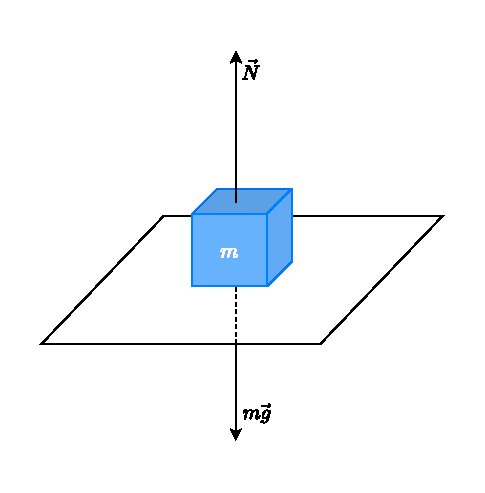
\includegraphics[width=0.5\linewidth]{res/svg/normalforce.drawio}
    \caption{Normal force on a plane}
    \label{fig:image6}
\end{figure}
Let's look deeper with another example. Imagine taking two masses $m_1$ and $m_2$ attached with an inextensible rope through an ideal pulley (massless and frictionless). Also consider the plane frictionless, we get this type of situation:
\begin{figure}[H]
    \centering
    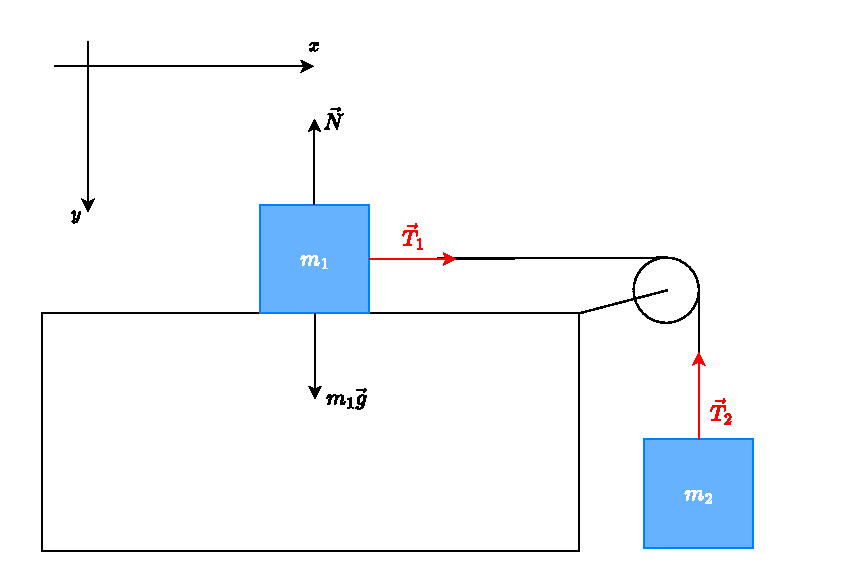
\includegraphics[width=0.6\linewidth]{res/svg/idealpulley.drawio}
    \caption{Normal force on a plane}
    \label{fig:image7}
\end{figure}
The ideal pulley gives us the information that $I\alpha = 0 \Rightarrow T_1 = T_2$. We also know that:
\[a_1 = a_2\]
This is the effect of the inextensible rope which is a \textbf{constraint} for the system. Solving Newton's equations leads to:
\begin{equation}
    \centering
\begin{cases}
T_1=T_2=m_1a \\[8pt]
m_2g -T =m_2a \\[8pt]
\end{cases} \Rightarrow a = \dfrac{m_2}{m_1+m_2}g
\end{equation}
\begin{definition}{Holonomic constraint}
  A constraint is said to be holonomic if it can be expressed as a function:
  \begin{equation}
    f(\vec{r}_1,\vec{r}_2, \,\dots\, ,\vec{r}_n,t) = 0
  \end{equation}
\end{definition}
For the inextensible rope the constraint can be expressed as $\dd{x}=\dd{y}$, but if we choose an appropriate frame of reference the condition can also simply be $x=y$, so the rope is a holonomic constraint such that:
\begin{equation}
    f(x,y)=0 \Rightarrow x-y=0
\end{equation}
If a constraint can be expressed as a function of the velocities it is said to be \textbf{semi-holonomic} and has a form such as:
\begin{equation}
    f(\dvec{r}_1,\dvec{r}_2, \,\dots\, ,\dvec{r}_n,t) = 0
\end{equation}
There are two main types of holonomic constraints:
\begin{itemize}
    \item \textbf{scleronomic} if it \underline{does not} depend on time explicitly \[f(\vec{r}_1,\vec{r}_2, \,\dots\, ,\vec{r}_n) = 0\]
    \item \textbf{rheonomic} if it \underline{does} depend on time explicitly \[f(\vec{r}_1,\vec{r}_2, \,\dots\, ,\vec{r}_n,t) = 0\]
\end{itemize}
A constraint allows us to express any coordinate as a function of the others, so, if we have $N$ particle we should have $3N$ coordinates, but if we have $K$ constraints the actual number of independent coordinates is:
\begin{equation}
    n = 3N-K = \text{dof (degrees of freedom)}
\end{equation}
\section{Virtual displacement}
\begin{definition}{Virtual displacement}
  A virtual displacement is an infinitesimal change in the configuration of the system that results in a change in the particle position compatible with the forces of constraint of the system \underline{at a given time}.
\end{definition}
To explain the difference between a virtual displacement and an actual displacement we can analyze the displacement of a moving object on an inclined plane with the angle changing over time:
\begin{figure}[H]
  \centering
  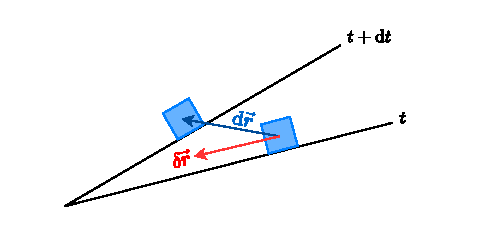
\includegraphics[width=0.5\linewidth]{res/svg/virtualdisplacement.drawio}
  \caption{Displacement and virtual displacement}
  \label{fig:image8}
\end{figure}
Where:
\begin{itemize}
    \item $\delta \vec{r}$ is the virtual displacement
    \item $\dd{\vec{r}}$ is the actual displacement
\end{itemize}
Now consider a system of particles at equilibrium so that:
\begin{equation}
    \vec{F}_i = 0\;\forall i
\end{equation}
The total force is composed of two separated parts:
\begin{itemize}
    \item Applied forces $\vec{F}^{(a)}_i$
    \item Constraint forces $\vec{f}_i$
\end{itemize}
At equilibrium we get:
\begin{equation}
    \begin{split}
      &\bigsum_i \vec{F}_i \cdot \delta \vec{r}_i = 0 \\[8pt]
      &\bigsum_i \brackets{\vec{F}^{(a)}_i + \vec{f}_i} \cdot \delta \vec{r}_i = \bigsum_i \vec{F}^{(a)}_i \cdot \delta \vec{r}_i + \bigsum_i \vec{f}_i \cdot \delta \vec{r}_i = 0
    \end{split}
\end{equation}
Now we consider only system with zero total virtual work, and we get:
\begin{equation}
    \begin{split}
      &\bigsum_i \vec{F}^{(a)}_i \cdot \delta \vec{r}_i + \cancel{\bigsum_i \vec{f}_i \cdot \delta \vec{r}_i} = 0 \\[8pt]
      &\bigsum_i \vec{F}^{(a)}_i \cdot \delta \vec{r}_i = 0
    \end{split}
\end{equation}
The last equation represents the condition of equilibrium for a system such that $\bigsum_i \vec{f}_i \cdot \delta \vec{r}_i = 0$ and is called \textbf{principle of virtual work}.
If the system \underline{is not} at equilibrium then we have:
\begin{equation}
    \vec{F}_i = \dvec{p}_i \Rightarrow \vec{F}_i - \dvec{p}_i = 0
\end{equation}
From which follows:
\begin{equation}
    \bigsum_i \brackets{\vec{F}_i - \dvec{p}_i} \cdot \delta \vec{r}_i = \bigsum_i \brackets{\vec{F}^{(a)}_i + \vec{f}_i - \dvec{p}_i} \cdot \delta \vec{r}_i = 0
\end{equation}
Now if the total virtual work of constraints is 0:
\begin{equation}
    \bigsum_i \brackets{\vec{F}^{(a)}_i - \dvec{p}_i} \cdot \delta \vec{r}_i + \cancel{\bigsum_i \vec{f}_i \cdot \delta \vec{r}_i} = 0
\end{equation}
And we get the so called \textbf{D'Alembert's principle}:
\begin{equation}  \label{D'Alembert_principle}
    \boxed{\bigsum_i \brackets{\vec{F}^{(a)}_i - \dvec{p}_i} \cdot \delta \vec{r}_i = 0}
\end{equation}
Now a problem arises. Since the $\delta \vec{r}_i$ are not independent in these coordinates we need to find a new set of coordinates that makes us able to make all the terms in the sum independent so we can establish that every single term is independently zero.
Those coordinates are called \textbf{generalized coordinates}.\\
Let us now consider only holonomic constraints so we have:
\begin{itemize}
    \item $N$ particles $\Rightarrow$ $3N$ coordinates
    \item $K$ constraints
\end{itemize}
So we actually have $n = 3N-K$ independent coordinates as we stated while talking about constraints in general. So we define the general coordinates:
\begin{equation}
    q_{\alpha}\;\forall\;\alpha = 1, \,\dots\, ,n
\end{equation}
As we stated all the original coordinates must only depend on the $q_{\alpha}$'s and (eventually) on time.
\begin{equation} \label{equations_of_transformation}
    \begin{cases}
        \vec{r}_1 = \vec{r}_1\brackets{q_1, \,\dots\, ,q_n,t}\\[8pt]
        \vec{r}_2 = \vec{r}_2\brackets{q_1, \,\dots\, ,q_n,t}\\[8pt]
         \,\dots\,  \\[8pt]
        \vec{r}_N = \vec{r}_N\brackets{q_1, \,\dots\, ,q_n,t}
    \end{cases}
\end{equation}
These are called the \textbf{equations of transformation}, and they have some properties:
\begin{itemize}
    \item explicitly contain the constraints
    \item can depend on time or not
    \item $q_{\alpha}$'s may not be lengths
    \item $q_{\alpha}$'s may not be grouped in vectors
    \item $q_{\alpha}$'s are scalars
\end{itemize}
An example of the use of generalized coordinates is the use of polar coordinates for the analysis of the pendulum system. In that case there are only 2 coordinates, but there is a constraint on the distance between the mass and the pole of the rotation, so we only have one independent coordinate:
\[q=\theta\]
Obviously it is possible to express general coordinates in terms of regular coordinates:
\begin{equation} \label{inverse_equations_of_transformation}
    \begin{cases}
        q_1 = q_1\brackets{\vec{r}_1, \,\dots\, ,\vec{r}_N,t}\\[8pt]
        q_2 = q_2\brackets{\vec{r}_1, \,\dots\, ,\vec{r}_N,t}\\[8pt]
         \,\dots\,  \\[8pt]
        q_n = q_n\brackets{\vec{r}_1, \,\dots\, ,\vec{r}_N,t}
    \end{cases}
\end{equation}

\chapter{Lagrange and Euler-Lagrange mechanics}
In this section we will discuss the main possible formulations of classical mechanics and their derivations. We also want to note that all the formulations are derived from Newton's equations and so they are completely equivalent to them if the conditions for their validity are satisfied.
\section{Lagrange equations}
Going back to \dalembertref, expressing in generalized coordinates:
\begin{equation}
    \bigsum_i \brackets{\vec{F}^{\cancel{(a)}}_i - \dvec{p}_i} \cdot \delta \vec{r}_i = 0
\end{equation}
We drop the (a) term for an easier notation, from now on we will write $\vec{F}_i$ knowing that we are indicating the applied force.
\begin{equation}
    \delta \vec{r}_i = \bigsum_{\alpha} \dfrac{\partial \vec{r}_i}{\partial q_{\alpha}} \delta q_{\alpha} + \cancel{\dfrac{\partial \vec{r}_i}{\partial t} \dd{t}}
\end{equation}
The partial derivative over time is zero since we are considering a fixed moment in time. The force term in \dalembertref\;becomes:
\begin{equation}
    \bigsum_i \vec{F}_i \cdot \bigsum_{\alpha} \dfrac{\partial \vec{r}_i}{\partial q_{\alpha}} \delta q_{\alpha} = \bigsum_{\alpha}\underbrace{\bigsum_{i} \vec{F}_i \cdot \dfrac{\partial \vec{r}_i}{\partial q_{\alpha}}}_{Q_{\alpha}} \delta q_{\alpha} = \bigsum_{\alpha}Q_{\alpha}\delta q_{\alpha}
\end{equation}
The terms $Q_{\alpha}$ are called \textbf{generalized components of the forces}.
Now let's consider the expression $\bigsum_i \dvec{p}_i \cdot \delta \vec{r}_i$. We know that:
\begin{itemize}
    \item $\dvec{p}_i = \dv{}{t}\brackets{m_i\vec{v}_i}$
    \item $\delta \vec{r}_i = \bigsum_{\alpha} \dfrac{\partial \vec{r}_i}{\partial q_{\alpha}}\delta q_{\alpha}$
\end{itemize}
Now, from the product rule:
\begin{equation} \label{e:total_deriv}
    \dv{}{t}\brackets{m_i\vec{v}_i \cdot \dfrac{\partial \vec{r}_i}{\partial q_{\alpha}}} = \dv{}{t}\brackets{m_i\vec{v}_i}\cdot \dfrac{\partial \vec{r}_i}{\partial q_{\alpha}} + m_i\vec{v}_i \cdot \dv{}{t}\brackets{\dfrac{\partial \vec{r}_i}{\partial q_{\alpha}}}
\end{equation}
From the last term we get:
\begin{equation} \label{e:funny_derivative_p1}
    \begin{split}
      m_i\vec{v}_i \cdot \dv{}{t}\brackets{\dfrac{\partial \vec{r}_i}{\partial q_{\alpha}}} &= m_i\vec{v}_i \cdot \bigsum_{\beta} \dfrac{\partial}{\partial \dot{q}_{\beta} }\brackets{\dfrac{\partial \vec{r}_i}{\partial q_{\alpha}}} q_{\beta} + \dfrac{\partial}{\partial t}\brackets{\dfrac{\partial \vec{r}_i}{\partial q_{\alpha}}} = \\[8pt]
      &= m_i\vec{v}_i \cdot \dfrac{\partial}{\partial q_{\alpha} }\underbrace{\left[\bigsum_{\beta} \dfrac{\partial \vec{r}_i}{\partial q_{\beta}} \dot{q}_{\beta} + \dfrac{\partial \vec{r}_i}{\partial t}\right]}_{\dvec{v}_i} = m_i\vec{v}_i \cdot \dfrac{\partial \vec{v}_i}{\partial q_{\alpha}}
    \end{split}
\end{equation}
We now aim to prove that the partial derivative with respect to alpha in the first term in \eqref{e:total_deriv} is:
\begin{equation}
    \dfrac{\partial \vec{r}_i}{\partial q_{\alpha}} = \dfrac{\partial \vec{v}_i}{\partial \dot{q}_{\alpha}}
\end{equation}
Deriving what we got in \eqref{e:funny_derivative_p1} we get:
\begin{equation}
    \begin{split}
      \dfrac{\partial \vec{v}_i}{\partial \dot{q}_{\alpha}} &= \dfrac{\partial }{\partial \dot{q}_{\alpha}} \brackets{\bigsum_{\beta}\dfrac{\partial \vec{r}_i}{\partial q_{\beta}} \dot{q}_{\beta} + \dfrac{\partial \vec{r}_i}{\partial t}} = \\[8pt]
      &= \bigsum_{\beta}\dfrac{\partial \vec{r}_i}{\partial q_{\beta}} \underbrace{\dfrac{\partial \dot{q}_{\beta}}{\partial \dot{q}_{\alpha}}}_{\delta_{\alpha \beta}}  + \cancel{\dfrac{\partial }{\partial \dot{q}_{\alpha}}\brackets{\dfrac{\partial \vec{r}_i}{\partial t}}} = \dfrac{\partial \vec{r}_i}{\partial q_{\alpha}}
    \end{split}
\end{equation}
Again, the first term of \eqref{e:total_deriv} can be rewritten as:
\begin{equation}
    \bigsum_i \dv{}{t}\brackets{m_i\vec{v}_i \cdot \dfrac{\partial \vec{r}_i}{\partial q_{\alpha}}} = \bigsum_i\dv{}{t}\brackets{m_i\vec{v}_i \cdot \dfrac{\partial \vec{v}_i}{\partial \dot{q}_{\alpha}}} = \dv{}{t}\left[\dfrac{\partial }{\partial \dot{q}_{\alpha}} \underbrace{\bigsum_i \brackets{\dfrac{1}{2}m_i \vec{v}_i \cdot \vec{v}_i}}_{T}\right]
\end{equation}
Similarly the last term in \eqref{e:total_deriv} is:
\begin{equation}
    \bigsum_im_i\vec{v}_i \cdot \dfrac{\partial \vec{v}_i}{\partial q_{\alpha}} = \dfrac{\partial }{\partial \dot{q}_{\alpha}} \underbrace{\bigsum_i \brackets{\dfrac{1}{2}m_i \vec{v}_i \cdot \vec{v}_i}}_{T}
\end{equation}
So we get:
\begin{equation}
    \bigsum_i \dv{}{t}\brackets{m_i\vec{v}_i}\cdot \dfrac{\partial \vec{r}_i}{\partial q_{\alpha}} = \dv{}{t}\dfrac{\partial T}{\partial \dot{q}_{\alpha}} - \dfrac{\partial T}{\partial q_{\alpha}}
\end{equation}
Going back to \dalembertref\;we get:
\begin{equation}
    \begin{split}
      \bigsum_i \brackets{\vec{F}_i - \dvec{p}_i} \cdot \delta \vec{r}_i &= \bigsum_{\alpha}Q_{\alpha}\delta q_{\alpha} - \bigsum_i \dv{}{t}\brackets{m_i\vec{v}_i} \cdot \bigsum_{\alpha}\dfrac{\partial \vec{r}_i}{\partial q_{\alpha}}\delta q_{\alpha} = \\[8pt]
      &= \bigsum_{\alpha}Q_{\alpha}\delta q_{\alpha} - \bigsum_{\alpha}\bigsum_i \dv{}{t}\brackets{m_i\vec{v}_i} \cdot \dfrac{\partial \vec{r}_i}{\partial q_{\alpha}}\delta q_{\alpha} = \\[8pt]
      &= \bigsum_{\alpha}Q_{\alpha}\delta q_{\alpha} - \bigsum_{\alpha}\brackets{\dv{}{t}\dfrac{\partial T}{\partial \dot{q}_{\alpha}} - \dfrac{\partial T}{\partial q_{\alpha}}}\delta q_{\alpha} = 0
    \end{split}
\end{equation}
All the terms are independent by construction so we get a set of equations which are called \textbf{Lagrange equations} $\heartsuit$:
\begin{equation} \label{Lagrange_equations}
    \boxed{\dv{}{t}\dfrac{\partial T}{\partial \dot{q}_{\alpha}} - \dfrac{\partial T}{\partial q_{\alpha}} = Q_{\alpha}}
\end{equation}
which must be satisfied $\forall \alpha$s.
Here are some basic properties of \lagrangeref :
\begin{itemize}
    \item There is a minimum of $n$ equations to solve
    \item They are $2^\circ$ order differential equations, this means that for every equation we need 2 initial conditions
    \item There is a total of $2n$ total initial conditions
\end{itemize}
\section{Euler-Lagrange equations}
From \lagrangeref\;it is easy to derive another formulation. Suppose that every force is expressed through a potential:
\begin{equation}
    \vec{F}_i = -\nabla_i V
\end{equation}
Since $V$ (the total potential) must be a function of only the coordinates $V = V(\vec{r}_i)$ we get that:
\begin{equation}
    Q_{\alpha} = \bigsum_i \vec{F}_i \cdot \dfrac{\partial \vec{r}_i}{\partial q_{\alpha}} = - \bigsum_i \nabla_i V \cdot \dfrac{\partial \vec{r}_i}{\partial q_{\alpha}} = -\partial{V}{q_{\alpha}}
\end{equation}
Rewriting \lagrangeref\;we get:
\begin{equation}
    \dv{}{t}\dfrac{\partial T}{\partial \dot{q}_{\alpha}} - \dfrac{\partial T}{\partial q_{\alpha}} + \partial{V}{q_{\alpha}} = 0
\end{equation}
If the potential does not depend on the generalized velocities we can subtract its derivative with respect to $\dot{q}_{\alpha}$, which will just be 0:
\begin{equation}
    \dv{}{t}\dfrac{\partial }{\partial \dot{q}_{\alpha}}[\underbrace{T-V}_\lagr ] - \dfrac{\partial}{\partial q_{\alpha}}[\underbrace{T-V}_\lagr ] = 0
\end{equation}
We define the Lagrange function or \textbf{Lagrangian} as:
\begin{equation}
    \lagr  = T - V
\end{equation}
Finally we can write the \textbf{Euler-Lagrange equations}:
\begin{equation} \label{Euler_Lagrange_equations}
    \boxed{\dv{}{t}\pdv{\lagr}{\dot{q}_{\alpha}} = \pdv{\lagr}{q_{\alpha}}}
\end{equation}
Here are some basic properties of \eleref :
\begin{itemize}
    \item They are $2^\circ$ order differential equations
    \item There is a total of $2n$ total initial conditions
    \item $\lagr = \lagr(q_{\alpha},\dot{q}_{\alpha},t)$ which means we have $2n+1$ variables
    \item $[\lagr] = \mathrm{J}$ but the Lagrangian is not the mechanical energy, it is just a mathematical tool
    \item If $\lagr$ is a Lagrangian of the system then $\tilde{\lagr} = \lagr + \mathrm{constant}$ is still Lagrangian
    \item If $\lagr$ is a Lagrangian of the system and $F\in \mathcal{C}^1$ is an arbitrary function of \underline{coordinates and time} then $\tilde{\lagr} = \lagr + \partial_t F$ is a Lagrangian
\end{itemize}
If we have two system, let's call them $A$ and $B$ then the Lagrangian of the total system $AB$ in general \underline{is not}:
\begin{equation}
    \lagr_{AB} = T_A + T_B - V_A - V_B - \underbrace{V_{AB}}_{\text{interaction term}}\neq \lagr_A + \lagr_B
\end{equation}
but if the systems interact weakly then:
\begin{equation}
    \lagr_{AB} \approx \lagr_A + \lagr_B
\end{equation}
If the potential $V$ \underline{does not} depend on time explicitly then the system is conservative:
\begin{equation}
    \begin{split}
      \delta W &= \bigsum_i \vec{F}_i \delta \vec{r}_i = \bigsum_i \vec{F}_i \bigsum_{\alpha}\dfrac{\partial \vec{r}_i}{\partial q_{\alpha}}\delta q_{\alpha} = \bigsum_{\alpha} Q_{\alpha}\delta q_{\alpha} = \\[8pt]
      &= -\bigsum_{\alpha} \partial{V}{q_{\alpha}}\delta q_{\alpha} = -\dd{V}
    \end{split}
\end{equation}
Instead if $V$ \underline{depends} on time explicitly we have that:
\begin{equation}
    \dd{V} = \bigsum_{\alpha} \partial{V}{q_{\alpha}}\delta q_{\alpha} + \dfrac{\partial V}{\partial t}\dd{t}
\end{equation}
The extra term appearing in $\dd{V}$ is not present in the expression for work, meaning that:
\begin{equation}
    W_{12} \neq -\int_{1}^{2}\dd{V} = V_1 - V_2
\end{equation}
so the system is not conservative.\\
In some cases (ex. Lorentz force) the force does not come from a "real" potential, we can then rewrite \eleref\;for a function called \textbf{generalized potential} $\mu$ such that:
\begin{equation}
    Q_{\alpha} = -\dfrac{\partial \mu}{\partial q_{\alpha}} +\dv{}{t}\dfrac{\partial \mu}{\partial \dot{q}_{\alpha}}
\end{equation}
Indeed, from \lagrangeref\;we get:
\begin{equation}
    \begin{split}
      \dv{}{t}\dfrac{\partial T}{\partial \dot{q}_{\alpha}} - \dfrac{\partial T}{\partial q_{\alpha}} &= -\dfrac{\partial \mu}{\partial q_{\alpha}} +\dv{}{t}\dfrac{\partial \mu}{\partial \dot{q}_{\alpha}} \\[8pt]
      \dv{}{t}\dfrac{\partial }{\partial \dot{q}_{\alpha}}[\underbrace{T-\mu}_{\lagr}] &- \dfrac{\partial}{\partial q_{\alpha}}[\underbrace{T-\mu}_{\lagr}] = 0 \\[8pt]
      \dv{}{t}\pdv{\lagr}{\dot{q}_{\alpha}} &= \pdv{\lagr}{q_{\alpha}}
    \end{split}
\end{equation}
where we defined a generalized Lagrangian $\lagr = T-\mu$. These are called \textbf{generalized Euler-Lagrange equations}.
\section{Derivation of Euler-Lagrange equations from Hamilton's principle}
A \textbf{monogenic system} is any system in which all the forces can be expressed through a (generalized) potential which depends on $q_{\alpha}$, $\dot{q}_{\alpha}$ and $t$.
\begin{definition}{Configuration space}
  Configuration space is the set of all the $q_{\alpha}$. It completely describes the position of each particle of the system at a givent time which, indeed, is the configuration of the system itself
\end{definition}
We can imagine the configuration space as an $n$-dimensional space in which the axes are the various $q_{\alpha}$.
Since each $q_{\alpha}$ changes with respect to time, the system describes a curve in the configuration space.\\
Let us consider two instants of time $t_1$ and $t_2$:
\begin{figure}[H]
    \centering
    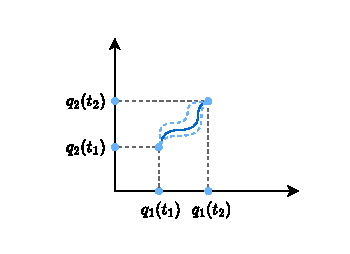
\includegraphics[width=0.6\linewidth]{res/svg/leastactionpath.drawio}
    \caption{Path of least action}
    \label{fig:image9}
\end{figure}
Then \textbf{Hamilton's principle} states that:
\begin{quote} \label{q:Hamilton_principle_quote} %Need to add principle ambient
    The path followed by a monogenic system in configuration space between $t_1$ and $t_2$ is the one for which the action $\action$ is stationary
\end{quote}
The action is defined as:
\begin{equation}
    \action = \int_{t_1}^{t_2}\lagr(q_{\alpha},\dot{q}_{\alpha},t) \dd{t}
\end{equation}
The units for actions are $[\action] = \mathrm{J\cdot s}$.\\ $\action$ is a \underline{functional} which is a "number" that depends on $q_{\alpha}$. Saying that $\action$ is stationary means that slightly changing the path does not change the action.\\
Now we aim to prove that the \hyperref[q:Hamilton_principle_quote]{Hamilton's principle} is true if and only if the \eleref\;are true.\\
\underline{Proof} H.P. $\Rightarrow$ E.L.E.\\
Let's give some conditions:
\begin{itemize}
    \item Call $\Gamma$ the real path
    \item Fix $t_1$ and $t_2$ but sligthly change the path in between
\end{itemize}
For the second point we need to change the real path of a small virtual displacement:
\begin{equation}
    q_{\alpha}(t) \longrightarrow q_{\alpha}(t) + \delta q_{\alpha}(t)
\end{equation}
However after varying the whole path, for the real path we get:
\begin{equation}
    \dot{q}_{\alpha} = \dfrac{\dd{q_{\alpha}}}{\dd{t}}
\end{equation}
for the changed path instead:
\begin{equation}
    \begin{split}
      \dot{q}_{\alpha} + \delta \dot{q}_{\alpha}(t) &= \dv{}{t}\brackets{q_{\alpha}(t) + \delta q_{\alpha}(t)} \\[8pt]
      \cancel{\dot{q}_{\alpha}} + \delta \dot{q}_{\alpha}(t) &= \cancel{\dot{q}_{\alpha}} + \dv{}{t}\brackets{\delta q_{\alpha}(t)} \\[8pt]
      \delta \dot{q}_{\alpha}(t) &= \dv{}{t}\brackets{\delta q_{\alpha}(t)}
    \end{split}
\end{equation}
Now let's evaluate the change on $\action$ and apply \hpquoteref\;which can be mathematically expressed as follows.\\\textbf{Hamilton's principle}:
\begin{equation} \label{e:Hamilton_principle}
    \delta \action = 0
\end{equation}
For the real path:
\begin{equation}
    \action = \int_{t_1}^{t_2}\lagr(q_{\alpha},\dot{q}_{\alpha},t) \dd{t}
\end{equation}
For the changed path:
\begin{equation}
    \tilde{\action} = \int_{t_1}^{t_2}\lagr(q_{\alpha}+\delta q_{\alpha},\dot{q}_{\alpha} + \delta \dot{q}_{\alpha},t) \dd{t}
\end{equation}
And so we get:
\begin{equation}
    \delta \action = \tilde{\action} - \action = \int_{t_1}^{t_2}\brackets{\lagr(q_{\alpha}+\delta q_{\alpha},\dot{q}_{\alpha} + \delta \dot{q}_{\alpha},t) - \lagr(q_{\alpha},\dot{q}_{\alpha},t)} \dd{t}
\end{equation}
The right-hand side of the equation basically has the numerator of the difference quotient:
\begin{equation}
    f'(x)h \sim f(x+h) - f(x)
\end{equation}
for arbitrarily small values of h, which in our case is the value of the virtual displacement $\delta$. Hence, we get:
\begin{equation}
    \delta \action = \int_{t_1}^{t_2}\bigsum_{\alpha}\brackets{\pdv{\lagr}{q_{\alpha}}\delta q_{\alpha} + \pdv{\lagr}{\dot{q}_{\alpha}} \underbrace{\delta \dot{q}_{\alpha}}_{\frac{\dd{}}{\dd{t}}\delta q_{\alpha}}} \dd{t} = 0
\end{equation}
Let's evaluate the second using integration by parts:
\begin{equation}
    \int_{t_1}^{t_2}\bigsum_{\alpha}\pdv{\lagr}{\dot{q}_{\alpha}} \dv{}{t}\delta q_{\alpha} \dd{t} = \cancel{\bigsum_{\alpha}\pdv{\lagr}{\dot{q}_{\alpha}} \delta q_{\alpha}\bigg|_{t_1}^{t_2}} - \int_{t_1}^{t_2}\bigsum_{\alpha}\dv{}{t}\brackets{\pdv{\lagr}{\dot{q}_{\alpha}}} \delta q_{\alpha} \dd{t}
\end{equation}
The term cancelled is zero since the displacement is zero in $t_1$ and $t_2$ for hypotesis. Hence, we get:
\begin{equation}
    \int_{t_1}^{t_2}\bigsum_{\alpha}\pdv{\lagr}{q_{\alpha}}\delta q_{\alpha} \dd{t} - \int_{t_1}^{t_2}\bigsum_{\alpha}\dv{}{t}\brackets{\pdv{\lagr}{\dot{q}_{\alpha}}} \delta q_{\alpha} \dd{t} = 0
\end{equation}
Since all the $\delta q_{\alpha}$ are independent we can pick any index $k$ and say that all the virtual displacements are zero except for the $k$-displacement, and we get:
\begin{equation}
    \int_{t_1}^{t_2}\dfrac{\partial \lagr}{\partial q_{k}}\delta q_{k} \dd{t} - \int_{t_1}^{t_2}\dv{}{t}\brackets{\dfrac{\partial \lagr}{\partial \dot{q}_{k}}} \delta q_{k} \dd{t} = 0
\end{equation}
Now we need a result which is called \textbf{Fundamental Lemma of the calculus of variation} which states that:\\
Taking any continuous function $M\in\mathcal{C}^0([a,b])$ and any function $\eta \in \mathcal{C}^2([a,b])$ such that $\eta(a) = \eta(b) = 0$ then it is true that:
\begin{equation} \label{e:Fundamental_lemma_variation_calculus}
    \int_{a}^{b}M(x)\eta(x)\dd{x} = 0 \Rightarrow M(x) = 0
\end{equation}
For the proof of this lemma we refer to the section (TBD).\\
In our case \eqref{e:Fundamental_lemma_variation_calculus} is satisfied for:
\begin{equation}
    \int_{t_1}^{t_2}\underbrace{\left[\dfrac{\partial \lagr}{\partial q_{k}} - \dv{}{t}\brackets{\dfrac{\partial \lagr}{\partial \dot{q}_{k}}}\right]}_{M} \underbrace{\delta q_{k}}_{\eta} \dd{t} = 0
\end{equation}
Hence:
\begin{equation}
    \begin{split}
      &\pdv{\lagr}{q_{\alpha}} - \dv{}{t}\brackets{\pdv{\lagr}{\dot{q}_{\alpha}}} = 0 \\[8pt]
      &\pdv{\lagr}{q_{\alpha}} = \dv{}{t}\brackets{\pdv{\lagr}{\dot{q}_{\alpha}}}
    \end{split}
\end{equation}
For any arbitrary $\alpha$. Hence, we proved that \hpquotemath\;implies \eleref.\\
It's trivial to prove the opposite since, repeating the passages of the first proof we arrive to:
\begin{equation}
    \delta \action = \int_{t_1}^{t_2}\bigsum_{\alpha}\left[\pdv{\lagr}{q_{\alpha}} - \dv{}{t}\brackets{\pdv{\lagr}{\dot{q}_{\alpha}}}\right] \delta q_{\alpha}
\end{equation}
But the terms in the brackets are all zero because of the \eleref. So we get:
\begin{equation}
    \delta \action = 0
\end{equation}
Which is precisely \hpquotemath.\\
Now that we established the relations between the \eleref\;and the \hpquotemath\;we are ready to prove that if $\lagr$ is a Lagrangian:
\begin{equation}
    \tilde{\lagr} = \lagr + \dfrac{\dd{F}}{\dd{t}}
\end{equation}
is a Lagrangian for the system. Evaluating the action for both Lagrangians we get:
\begin{equation}
    \tilde{\action} = \int_{t_1}^{t_2}\lagr \dd{t} + \int_{t_1}^{t_2}\dfrac{\dd{F}}{\dd{t}} \dd{t}
\end{equation}
\begin{equation}
    \action = \int_{t_1}^{t_2}\lagr \dd{t}
\end{equation}
The difference of action for the new Lagrangian is:
\begin{equation}
    \delta \tilde{\action} = \int_{t_1}^{t_2}\dfrac{\dd{F}}{\dd{t}} \dd{t} = F(t_2) - F(t_1)
\end{equation}
And so we get:
\begin{equation}
    \delta \tilde{\action} = \delta \action + \cancel{\delta(F(t_2) - F(t_1))}
\end{equation}
The variation between the values of $F$ is obviously zero since their difference is just a constant number that comes from the integral. So if \hpquotemath\;holds for $\lagr$ we have:
\begin{equation}
    \delta \tilde{\action} = \delta \action = 0
\end{equation}
And so $\tilde{\lagr}$ is a Lagrangian for the system.\\
\section{Examples (WIP)}
\section{The energy function}
Let's now discuss the energy of a system. The Lagrangian $\lagr$ has the dimensions of an energy, but it \underline{is not} the total energy.
\begin{equation}
    \lagr = T - V \cancel{\Leftrightarrow} E = T + V
\end{equation}
We can evaluate the derivative of the Lagrangian and see what we get:
\begin{equation}
    \dfrac{\dd{\lagr}}{\dd{t}} = \bigsum_{\alpha}\brackets{\pdv{\lagr}{q_{\alpha}}\dot{q}_{\alpha} + \pdv{\lagr}{\dot{q}_{\alpha}}\ddot{q}_{\alpha}} + \dfrac{\partial \lagr}{\partial t}
\end{equation}
If \eleref\;hold then we have:
\begin{equation}
    \dfrac{\dd{\lagr}}{\dd{t}} = \bigsum_{\alpha}\underbrace{\left[\dv{}{t}\brackets{\pdv{\lagr}{\dot{q}_{\alpha}}}\dot{q}_{\alpha} + \pdv{\lagr}{\dot{q}_{\alpha}}\ddot{q}_{\alpha}\right]}_{\text{total time derivative}} + \dfrac{\partial \lagr}{\partial t} =
\end{equation}
\begin{equation}
 = \dv{}{t}\bigsum_{\alpha}\pdv{\lagr}{\dot{q}_{\alpha}}\dot{q}_{\alpha} + \dfrac{\partial \lagr}{\partial t}
\end{equation}
So in general:
\begin{equation}
    \dfrac{\dd{\lagr}}{\dd{t}} \neq 0
\end{equation}
even if the partial derivative of $\lagr$ with respect to time is zero. But we can define a quantity $h$ called \textbf{energy function}:
\begin{equation}
    h \defineeq \bigsum_{\alpha}\pdv{\lagr}{\dot{q}_{\alpha}}\dot{q}_{\alpha} - \lagr
\end{equation}
and so we have:
\begin{equation}
    \dfrac{\dd{h}}{\dd{t}} = -\dfrac{\partial \lagr}{\partial t}
\end{equation}
Obviously $h$ is a constant of motion if and only if the partial derivative with respect to time of the Lagrangian is 0:
\begin{equation}
    h\;\text{is conserved} \iff \dfrac{\dd{h}}{\dd{t}} = 0 \iff \dfrac{\partial \lagr}{\partial t} = 0
\end{equation}
Saying that $\lagr$ does not depend on time explicitly means that the potential $V$ does not depend on time and also:
\begin{itemize}
    \item Constraints depending on time $\Rightarrow$ $\lagr$ depends on time
    \item Constraints not depending on time $\Rightarrow$ $\lagr$ does not depend on time
\end{itemize}
Now we want to prove that $h$ is the total energy if these conditions hold:
\begin{enumerate}
    \item Transformation equations do not depend on time
    \item The potential $V$ does not depend on time
\end{enumerate}
Let's further analyse condition (1). Writing the kinetic energy $T$ we get:
\begin{equation}
    T = \dfrac{1}{2}\bigsum_i m_i v_i^2 = \dfrac{1}{2}\bigsum_i m_i \dvec{r}_i \cdot \dvec{r}_i
\end{equation}
The time derivative of $r_i(q_{\alpha},t)$ is:
\begin{equation}
    \dvec{r}_i = \dfrac{\dd{\vec{r}_i}}{\dd{t}} = \bigsum_{\alpha}\dfrac{\partial \vec{r}_i}{\partial q_{\alpha}}\dot{q}_{\alpha} + \dfrac{\partial \vec{r}_i}{\partial t}
\end{equation}
Hence we have:
\begin{equation}
    T = \dfrac{1}{2}\bigsum_i m_i \left[\bigsum_{\alpha}\dfrac{\partial \vec{r}_i}{\partial q_{\alpha}}\dot{q}_{\alpha} + \dfrac{\partial \vec{r}_i}{\partial t}\right] \cdot \left[\bigsum_{\beta}\dfrac{\partial \vec{r}_i}{\partial q_{\beta}}\dot{q}_{\beta} + \dfrac{\partial \vec{r}_i}{\partial t}\right] =
\end{equation}

\begin{equation}
    \begin{split}
        = \dfrac{1}{2}\bigsum_i m_i \bigsum_{\alpha}\bigsum_{\beta}\dfrac{\partial \vec{r}_i}{\partial q_{\alpha}}\cdot\dfrac{\partial \vec{r}_i}{\partial q_{\beta}}\dot{q}_{\alpha}\dot{q}_{\beta} + \dfrac{1}{2}\bigsum_i m_i \dfrac{\partial \vec{r}_i}{\partial t} \cdot \dfrac{\partial \vec{r}_i}{\partial t} +\\
        + \dfrac{1}{2}\bigsum_i m_i \bigsum_{\alpha}\dfrac{\partial \vec{r}_i}{\partial q_{\alpha}} \cdot \dfrac{\partial \vec{r}_i}{\partial t} \dot{q}_{\alpha} + \dfrac{1}{2}\bigsum_i m_i \bigsum_{\beta}\dfrac{\partial \vec{r}_i}{\partial q_{\beta}} \cdot \dfrac{\partial \vec{r}_i}{\partial t}\dot{q}_{\beta}
    \end{split}
\end{equation}
The terms on the second line are actually the same since summing over $\alpha$ or $\beta$ is actually the same. Let us now define some quantities for a shorter notation:
\begin{equation}
    \begin{split}
        T_{\alpha \beta} \defineeq \bigsum_i m_i \dfrac{\partial \vec{r}_i}{\partial q_{\alpha}}\cdot\dfrac{\partial \vec{r}_i}{\partial q_{\beta}}\\
        T_{\alpha} \defineeq \dfrac{1}{2} \bigsum_i m_i \dfrac{\partial \vec{r}_i}{\partial q_{\alpha}} \cdot \boxed{\dfrac{\partial \vec{r}_i}{\partial t}}\\
        T_0 \defineeq \dfrac{1}{2}\bigsum_i m_i \boxed{\dfrac{\partial \vec{r}_i}{\partial t} \cdot \dfrac{\partial \vec{r}_i}{\partial t}}
    \end{split}
\end{equation}
The quantities $T_{\alpha}$ and $T_0$ are zero if the transformation equations do not depend on time explicitly since the partial derivative with respect to time of $\vec{r}_i$ is zero. Rewriting the kinetic energy we have:
\begin{equation}
    T = \dfrac{1}{2}\bigsum_{\alpha}\bigsum_{\beta}T_{\alpha \beta}\dot{q}_{\alpha}\dot{q}_{\beta} + \cancel{\bigsum_{\alpha}T_{\alpha}\dot{q}_{\alpha}} + \cancel{T_0}
\end{equation}
\begin{equation} \label{e:kinetic_energy}
    T = \dfrac{1}{2}\bigsum_{\alpha}\bigsum_{\beta}T_{\alpha \beta}\dot{q}_{\alpha}\dot{q}_{\beta}
\end{equation}
And so $T$ is a quadratic function of the generalized velocities.\\
Now let's analyse condition (2). To start we can remember this:
\begin{equation}
    \pdv{\lagr}{\dot{q}_{\alpha}} = \dfrac{\partial T}{\partial \dot{q}_{\alpha}} - \cancel{\partial{V}{\dot{q}_{\alpha}}}
\end{equation}
since $V$ does not depend on the generalized velocities. Now substituting \eqref{e:kinetic_energy} we get:
\begin{equation}
    h = \bigsum_{\gamma}\dfrac{\partial T}{\partial \dot{q}_{\gamma}} - \lagr = \bigsum_{\gamma}\dfrac{\partial}{\partial \dot{q}_{\gamma}}\bbrackets{\dfrac{1}{2}\bigsum_{\alpha}\bigsum_{\beta}\underbrace{T_{\alpha \beta}}_{\cancel{\propto} \dot{q}_{\alpha}, \dot{q}_{\beta}}\dot{q}_{\alpha}\dot{q}_{\beta}}  - \lagr =
\end{equation}
We can bring the partial derivative inside the sum:
\begin{equation}
    h = \dfrac{1}{2}\bigsum_{\gamma}\bigsum_{\alpha}\bigsum_{\beta}T_{\alpha \beta}\bbrackets{\underbrace{\dfrac{\partial \dot{q}_{\alpha}}{\partial \dot{q}_{\gamma}}}_{\delta_{\alpha \gamma}}\dot{q}_{\beta} + \underbrace{\dfrac{\partial \dot{q}_{\beta}}{\partial \dot{q}_{\gamma}}}_{\delta_{\beta \gamma}}\dot{q}_{\alpha}} - \lagr
\end{equation}
If we split out the terms of the sum we can cancel out the sum over $\alpha$ in the first term due to the Kronecker delta. Similarly, we can cancel out the sum over $\beta$. We need to remind that we also need to switch the cancelled indexes with $\gamma$ since those are the remaining terms.
\begin{equation}
    \bigsum_{\gamma}\cancel{\bigsum_{\alpha}}\bigsum_{\beta}T_{\alpha \beta }\cancel{\delta_{\alpha \gamma}}\dot{q}_{\beta} = \bigsum_{\gamma}\bigsum_{\beta}T_{\gamma \beta }\dot{q}_{\beta}
\end{equation}
So we get:
\begin{equation}
    h = \underbrace{\dfrac{1}{2}\bigsum_{\gamma}\bigsum_{\beta}T_{\gamma \beta }\dot{q}_{\beta}}_{T} + \underbrace{\dfrac{1}{2}\bigsum_{\gamma}\bigsum_{\alpha}T_{\gamma \alpha }\dot{q}_{\alpha}}_{T} - \lagr = 2T - (T-V) = T + V = E
\end{equation}
And so conditions (1) and (2) really are the conditions for $h$ to be the total energy of the system $E$. The conditions for $h$ to be the energy and for $h$ to be conserved do not necessarily match, so we can have all the possible cases:
\begin{itemize}
    \item $h$ is the energy and it is conserved
    \item $h$ is the energy but it is not conserved
    \item $h$ is not the energy but it is conserved
    \item $h$ is not the energy and it is not conserved
\end{itemize}
\section{Conservation of the total linear momentum}
Let's now talk about the conservation of linear momenta. In the Lagrange formalism the role of linear momentum is done by the \textbf{generalized momentum} conjugate to $q_{\alpha}$:
\begin{equation}
    p_{\alpha} \defineeq \pdv{\lagr}{\dot{q}_{\alpha}}
\end{equation}
which can also be called \textbf{canonical momentum}. The generalized momentum may not correspond to the linear momentum we get from Newton's equations. We can show that for an easy example the two quantities correspond.\\
Let's define the Lagrangian as:
\begin{equation}
    \lagr = \dfrac{1}{2}m(\dot{x}^2 + \dot{y}^2 + \dot{z}^2) - V(x,y,z)
\end{equation}
This might be an example for an easy "Physics I-like" system (for example a falling object). We evaluate the generalized momentum conjugate to x and get:
\begin{equation}
    p_x = \dfrac{\partial \lagr}{\partial \dot{x}} = m\dot{x}
\end{equation}
which is indeed the linear momentum found by using Newton's equations.\\
If we go back to \eleref\;and \lagrangeref\;we can identify the term $p_{\alpha}$ inside those equations. If they hold (remember we need to ask for a potential independent of the velocities) then we can write:
\begin{equation}
    \dfrac{\dd{p_{\alpha}}}{\dd{t}} = \pdv{\lagr}{q_{\alpha}} \Rightarrow \dot{p}_{\alpha} = \pdv{\lagr}{q_{\alpha}}
\end{equation}
If only the potential does depend on the coordinates and $T$ does not then we can also write:
\begin{equation}
    \dot{p}_{\alpha} = \pdv{[\cancel{T}-V]}{q_{\alpha}} = -\pdv{V}{q_{\alpha}}
\end{equation}
If $V$ does not depend on the velocities we also have:
\begin{equation}
    -\pdv{V}{q_{\alpha}} = Q_{\alpha}
\end{equation}
\begin{equation}
    \boxed{\dot{p}_{\alpha} = Q_{\alpha}}
\end{equation}
This is the corresponding relation for $\vec{F} = \dvec{p}$ in Newton's equations. If $V$ depends on $\dot{q}_{\alpha}$ we get:
\begin{equation}
    \dv{}{t}\pdv{V}{\dot{q}_{\alpha}}-\pdv{V}{q_{\alpha}} = Q_{\alpha}
\end{equation}
Let us now define what \textbf{cyclic coordinates} are.
\begin{equation}
    q_{\alpha}\;\text{is cyclic} \iff \pdv{\lagr}{q_{\alpha}} = 0
\end{equation}
If $q_{\alpha}$ is cyclic and \eleref\;are true we have:
\begin{equation}
    \dv{}{t} \pdv{\lagr}{\dot{q}_j} - \cancel{\pdv{\lagr}{q_{\alpha}}} = 0
\end{equation}
\begin{equation}
    \dot{p}_{\alpha} = 0
\end{equation}
This means that if a coordinate is cyclic its corresponding generalized momentum is conserved.\\
Now let $q_j$ be a \textbf{collective coordinate} such that $\delta q_j$ represents an infinitesimal displacement of the system \underline{as a whole}.
\begin{figure}[H]
    \centering
    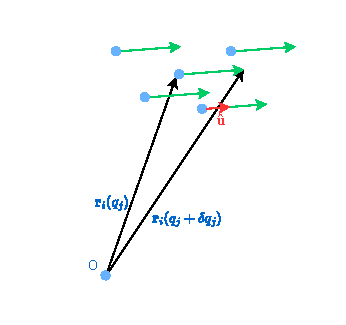
\includegraphics[width=0.4\linewidth]{res/svg/collectivecoord.drawio}
    \caption{Collective coordinate}
\end{figure}
If this is the case all the particles are moving parallel to a single unit vector $\hat{u}$:
\begin{equation}
    \hat{u} = \dfrac{\partial \vec{r}_i}{\partial q_j}
\end{equation}
\begin{equation}
    \delta \vec{r}_i = \delta q_j \hat{u}
\end{equation}
Also $q_j$ cannot appear in the expression of $T$, hence:
\begin{equation}
    \pdv{T}{q_j}=0
\end{equation}
Changing $q_j$ is a translation that leaves everything untouched (like moving the origini of the axis). Now consider $V=V(q_{\alpha},\cancel{\dot{q}_{\alpha}},t)$:
\begin{equation}
    -\pdv{V}{q_{\alpha}} = Q_{\alpha}
\end{equation}
Let's consider \eleref\;for $q_j$:
\begin{equation}
    \dv{}{t}\underbrace{\pdv{\lagr}{\dot{q}_j}}_{p_j} - \underbrace{\pdv{\lagr}{q_j}}_{-\frac{\partial V}{\partial q_j}} = 0
\end{equation}
\begin{equation} \label{e:ele_for_qj}
    \dv{}{t}p_j = -\pdv{V}{q_j} = Q_j
\end{equation}
Remembering the definition of $Q_j$:
\begin{equation}
    Q_j = \bigsum_i \vec{F}_i \cdot \underbrace{\pdv{\vec{r}_i}{q_j}}_{\hat{u}} = \vec{F}\cdot \hat{u}
\end{equation}
Similarly from the definition of $p_j$:
\begin{equation}
    p_j = \pdv{\lagr}{\dot{q}_j} = \pdv{}{\dot{q}_j}\brackets{\dfrac{1}{2}\bigsum_i m_i \vec{r}_i^{\;2}} = \dfrac{1}{2}\bigsum_i m_i \pdv{}{\dot{q}_j}(\vec{r}_i^2) = \bigsum_i m_i \vec{r}_i \cdot \underbrace{\pdv{\vec{r}_i}{\dot{q}_j}}_{\hat{u}}
\end{equation}
\begin{equation}
    p_j = \vec{P}\cdot\hat{u}
\end{equation}
Going back to \eqref{e:ele_for_qj}:
\begin{equation}
    \dv{}{t}(\vec{P}\cdot\hat{u}) = \vec{F}\cdot \hat{u}
\end{equation}
If $q_j$ is also a cyclic coordinate we have:
\begin{equation}
    \pdv{\lagr}{q_j} = 0 \Rightarrow \pdv{[\cancel{T}-V]}{q_j} = \pdv{V}{q_j} = 0
\end{equation}
From this immediately follows:
\begin{equation}
    Q_j = 0 \Rightarrow \dv{}{t}(p_j) = \dv{}{t}(\vec{P}\cdot\hat{u}) = 0
\end{equation}
So if $q_j$ is a cyclic and collective coordinate the generalized momentum conjugate to $q_j$ si conserved.
\section{Conservation of the total angular momentum}
Let's consider a specific coordinate $q_j$ such that $\delta q_j$ is a rigid rotation of the system as a whole, about a certain axis as shown:
\\\textbf{IMAGE}\\
We can see that $\delta \vec{r}_i$ is a tangential displacement. If we use the angle $\theta$ as our coordinate we can write:
\begin{equation}
    \dv{\vec{r}_i}{t} = \dv{\theta}{t} \hat{u} \cross \vec{r}_i = \dot{q}_j \hat{u} \cross \vec{r}_i
\end{equation}
From which follows:
\begin{equation}
    \delta \vec{r}_i = \delta q_j \hat{u} \cross \vec{r}_i \Rightarrow \pdv{\vec{r}_i}{q_j} = \hat{u} \cross \vec{r}_i
\end{equation}
Also $q_j$ cannot appear in the expression of $T$, hence:
\begin{equation}
    \pdv{T}{q_j} = 0
\end{equation}
Now we consider a system such that $V = V(q_{\alpha},\cancel{\dot{q}_{\alpha}},t)$ and write \eleref\;for $q_j$:
\begin{equation} \label{e:ele_for_angular_momentum}
    \begin{split}
        \dv{}{t}\pdv{\lagr}{\dot{q}_j} - \pdv{\lagr}{q_j} = 0\\
        \dv{}{t}\underbrace{\pdv{T}{\dot{q}_j}}_{p_j} - \bbrackets{\underbrace{- \pdv{V}{q_j}}_{Q_j}} = 0
    \end{split}
\end{equation}
Let's explicitly write $Q_j$:
\begin{equation}
    Q_j = \bigsum_i \vec{F}_i \cdot \pdv{\vec{r}_i}{q_j} = \bigsum_i \vec{F}_i \cdot \hat{u} \cross \vec{r}_i
\end{equation}
Inside the summation we have a triple product, hence we can exploit the fact that $\hat{u}$ does not depend on $i$ and also the invariance of the triple product with respect to circular shifts:
\begin{equation}
    \vec{a} \cdot \vec{b} \cross \vec{c} = \vec{c} \cdot \vec{a} \cross \vec{b} = \vec{b} \cdot \vec{c} \cross \vec{a}
\end{equation}
And so we get:
\begin{equation}
    Q_j = \hat{u} \cdot \underbrace{\bigsum_i \vec{r}_i \cross \vec{F}_i}_{\vec{\tau}} = \hat{u} \cdot \vec{\tau}
\end{equation}
Now let's analyse the partial derivative of the kinetic energy:
\begin{equation}
    \pdv{T}{\dot{q}_j} = \pdv{}{\dot{q}_j}\brackets{\dfrac{1}{2}\bigsum_i m_i \vec{r}_i^{\;2}} = \bigsum_i m_i \vec{r}_i \cdot \pdv{\vec{r}_i}{\dot{q}_j} = \bigsum_i m_i \vec{r}_i \cdot \hat{u} \cross \vec{r}_i
\end{equation}
Again we exploit the properties of the triple product and get:
\begin{equation}
    \pdv{T}{\dot{q}_j} =   \hat{u} \cdot \underbrace{\bigsum_i \vec{r}_i \cross m_i \vec{r}_i}_{\vec{L}_0} = \hat{u} \cdot \vec{L}_0
\end{equation}
Finally we can substitute back into \eqref{e:ele_for_angular_momentum}:
\begin{equation}
    \dv{}{t}\brackets{\vec{L}_0 \cdot \hat{u}} = \vec{\tau} \cdot \hat{u}
\end{equation}
This means that if the total torque about a generic axis is zero, then the total angular momentum about that axis is conserved. For example if we let $\hat{u} = \hat{z}$:
\begin{equation}
    \tau_z = 0 \Rightarrow L_z\;\text{is conserved}
\end{equation}
We then notice that if $q_j$ is a cyclic coordinate we have:
\begin{equation}
    Q_j = -\pdv{V}{q_j} = 0 \Rightarrow \vec{\tau} \cdot \hat{u} = 0 \Rightarrow \vec{L}_0 \cdot \hat{u}\;\text{is conserved}
\end{equation}
\section{Noether's theorem}
In the last two sections we arrived to these conclusions:
\begin{itemize}
    \item The conservation of the total momentum is due to an invariance of $\lagr$ to translations
    \item The conservation of the momentum along an axis is due to an invariance of $\lagr$ to translation along that axis
    \item The conservation of the total angular momentum is due to an invariance of $\lagr$ to rotations
    \item The conservation of the angular momentum along an axis is due to an invariance of $\lagr$ to rotations along that axis
    \item If $\lagr$ is invariant with respect to time the energy function is conserved
\end{itemize}
We can easily see the "pattern" arising from those conclusions. Those are all examples of a famous theorem which states:
\begin{theorem}{Noether's theorem}
    For every invariance of $\lagr$ there is a conserved quantity
\end{theorem}

\chapter{Hamilton's mechanics}
\section{Hamilton's equations}
Now let's recap what we established with the differente pictures of classical mechanics that we discussed until now.
\begin{itemize}
    \item \eleref\;are a set of $n$ differential equations of $2^\circ$ order with $2n$ initial conditions
    \item When a coordinate is cyclic then: \begin{equation}
        p_{\alpha} = \pdv{\lagr}{\dot{q}_{\alpha}}\;\text{is conserved}
    \end{equation}
    but $p_{\alpha}$ is not a quantity of the Lagrangian
    \item even if $p_\alpha$ is conserved we still have $\dot{q}_{\alpha}$ as an ``extra'' term in the Lagrangian
\end{itemize}
We want to use a space differente from the configuration space in order to get rid of a useless term when a coordinate is cyclic. We then introduce a new concept.
\begin{definition}{Phase space}
  Phase space is a $2n$-dimensional space in which each point represents the \underline{state} of the system $\{q_{\alpha},p_{\alpha}\}$.
\end{definition}
Here are the fundamental differences between Lagrange formulation and Hamilton formulation of classical mechanics:
\begin{table}[H]
    \centering
    \begin{tabular}{lll}
        \underline{Lagrange} & $\longrightarrow$ &\underline{Hamilton}\\[8pt]
        $\lagr=\lagr(q_{\alpha},\dot{q}_{\alpha},t)$ & &$\hamfun=\hamfun(q_{\alpha},p_{\alpha},t)$\\[8pt]
        Configuration space & &Phase space\\[8pt]
        $n$ dimensions & &$2n$ dimensions
    \end{tabular}
\end{table}
Since we want to find a new function related to the Lagrangian that contains $p_{\alpha}$ as a variable instead of $\dot{q}_{\alpha}$, we need to introduce a certain type of transformation.\\
\textbf{Legendre transformations} are able to write a function $f(x,y)$ as a function $g(u,y)$ where:
\begin{equation}
    \dd{f} = \underbrace{\pdv{f}{x}}_u \dd{x} + \underbrace{\pdv{f}{y}}_v \dd{y} = u\dd{x} + v\dd{y}
\end{equation}
From this first relation we can work on the term $u\dd{x}$:
\begin{equation}
    \dd{(ux)} = u\dd{x} + x\dd{u} \Rightarrow u\dd{x} = \dd{(ux)} - x\dd{u}
\end{equation}
Then it is easy to see that a function $g = f-ux$ satisfies our conditions, and so we have:
\begin{equation}
    \dd{g} = \dd{(f-ux)} = - x\dd{u} + v\dd{y} \Rightarrow \begin{cases}
        \partial_{u} g = -x\\
        \partial_{y} g = v
    \end{cases}
\end{equation}
Let's try to apply Légendre transformations to the Lagrangian:
\begin{equation}
    \dd{\lagr} = \bigsum_{\alpha} \pdv{\lagr}{q_{\alpha}}\dd{q_{\alpha}} + \bigsum_{\alpha} \underbrace{\pdv{\lagr}{\dot{q}_{\alpha}}}_{p_{\alpha}}\dd{\dot{q}_{\alpha}} + \pdv{\lagr}{t}\dd{t}
\end{equation}
We then applied Légendre transformations to $\lagr$:
\begin{equation} \label{e:legendre_hamilton}
    \dd{\brackets{\lagr - \bigsum_{\alpha} p_{\alpha}\dot{q}_{\alpha}}} = \bigsum_{\alpha} \pdv{\lagr}{q_{\alpha}}\dd{q_{\alpha}} - \bigsum_{\alpha} \dot{q}_{\alpha}\dd{p_{\alpha}} + \pdv{\lagr}{t}\dd{t}
\end{equation}
And so if we define a function $\hamfun$ called \textbf{Hamiltonian} (or Hamilton function):
\begin{equation}
    \hamfun \defineeq \bigsum_{\alpha} p_{\alpha}\dot{q}_{\alpha} -\lagr
\end{equation}
Then \eqref{e:legendre_hamilton} becomes:
\begin{equation}
    \begin{split}
        -\dd{\hamfun} = \bigsum_{\alpha} \underbrace{\pdv{\lagr}{q_{\alpha}}}_{\dot{p}_{\alpha}}\dd{q_{\alpha}} - \bigsum_{\alpha} \dot{q}_{\alpha}\dd{p_{\alpha}} + \pdv{\lagr}{t}\dd{t}\\
        \dd{\hamfun} = -\bigsum_{\alpha} \dot{p}_{\alpha}\dd{q_{\alpha}} + \bigsum_{\alpha} \dot{q}_{\alpha}\dd{p_{\alpha}} - \pdv{\lagr}{t}\dd{t}\\
    \end{split}
\end{equation}
But also it is genrally true that:
\begin{equation}
    \dd{\hamfun} = \bigsum_{\alpha} \pdv{\hamfun}{q_{\alpha}}\dd{q_{\alpha}} + \bigsum_{\alpha} \pdv{\hamfun}{p_{\alpha}}\dd{p_{\alpha}} + \pdv{\hamfun}{t}\dd{t}
\end{equation}
The two equations must be equal so we get \textbf{Hamilton's canonical equations}:
\begin{equation} \label{hamilton_equations}
    \boxed{
    \begin{aligned}
        \pdv{\hamfun}{q_{\alpha}} &= -\dot{p}_{\alpha}\\
        \pdv{\hamfun}{p_{\alpha}} &=\;\;\;\dot{q}_{\alpha}\\
        \pdv{\hamfun}{t} &= -\pdv{\lagr}{t}
    \end{aligned}}
\end{equation}
This is a system of $2n (+1)$ equations, but they are first order ODEs so we have $2n$ initial conditions as in \lagrangeref. With this formulation we have one important advantage: if $q_j$ is cyclic then $\dot{p} = 0$, and we don't need to solve one of the differential equations.
This means that we only need $2n-1$ initial conditions. Same goes for any other cyclic coordinate, and so we have $2n-p$ initial conditions with $p$ being the number of cyclic coordinates.\\
Now let's remember the definition of the energy function:
\begin{equation}
    h = \bigsum_{\alpha}\underbrace{\pdv{\lagr}{q_{\alpha}}}_{p_{\alpha}}\dot{q}_{\alpha} - \lagr
\end{equation}
So we can say that the only difference between the energy function $h$ and the Hamiltonian $\hamfun$ is the fact that the first lives in the configuration space, the latter instead lives in the phase space.
To further convince ourselves of this fact we can evaluate the total derivative of $\hamfun$ over time:
\begin{equation}
    \begin{split}
        \dv{\hamfun}{t} &= \bigsum_{\alpha}\underbrace{\pdv{\hamfun}{q_{\alpha}}}_{-\dot{p}_{\alpha}}\dot{q}_{\alpha} + \bigsum_{\alpha}\underbrace{\pdv{\hamfun}{p_{\alpha}}}_{\dot{q}_{\alpha}}\dot{p}_{\alpha} + \pdv{\hamfun}{t} \\
        \dv{\hamfun}{t} &= \pdv{\hamfun}{t} = -\pdv{\lagr}{t}
    \end{split}
\end{equation}
So we get that $\hamfun$ will be the energy and/or will be conserved in the same situations of the energy function.
\section{Hamilton's equations through Hamilton's principle}
To derive \hamiltonref\;we can also exploit \hpquotemath\;starting from:
\begin{equation}
    \action = \int_{t_1}^{t_2}\lagr \dd{t}
\end{equation}
Using the same definition for $\hamfun$ that we previously used:
\begin{equation}
    \hamfun = \bigsum_{\alpha}p_{\alpha}\dot{q}_{\alpha} - \lagr
\end{equation}
We get:
\begin{equation} \label{e:deltaS_hamilton}
    \delta \action = \int_{t_1}^{t_2}\bbrackets{\bigsum_{\alpha}\delta p_{\alpha}\dot{q}_{\alpha} + \bigsum_{\alpha} p_{\alpha} \underbrace{\delta \dot{q}_{\alpha}}_{\frac{\dd{}}{\dd{t}}\delta q_{\alpha}} - \bigsum_{\alpha} \pdv{\hamfun}{q_{\alpha}} \delta q_{\alpha}- \bigsum_{\alpha} \pdv{\hamfun}{p_{\alpha}} \delta p_{\alpha}} \dd{t}
\end{equation}
We apply the product rule on the second member:
\begin{equation}
    \bigsum_{\alpha} p_{\alpha} \dv{}{t}\delta q_{\alpha} = \bigsum_{\alpha} \bigg[ \dv{}{t} \brackets{p_{\alpha} \delta q_{\alpha}} -  \delta q_{\alpha}\dv{}{t}p_{\alpha}\bigg]
\end{equation}
Integrating the first term we get:
\begin{equation}
    \int_{t_1}^{t_2} \bigsum_{\alpha} \dv{}{t} \brackets{p_{\alpha} \delta q_{\alpha}} \dd{t} = \bigsum_{\alpha} p_{\alpha} \delta q_{\alpha} \bigg|_{t_1}^{t_2} = 0
\end{equation}
This is zero because in \hpquotemath\;we assumed that the virtual displacement at the extreme points is zero. So we can rewrite \eqref{e:deltaS_hamilton} putting in evidence the common terms:
\begin{equation}
    \begin{split}
        \delta \action &= \int_{t_1}^{t_2}\bbrackets{\bigsum_{\alpha}\delta p_{\alpha}\dot{q}_{\alpha} - \bigsum_{\alpha} \delta q_{\alpha}\dot{p}_{\alpha} - \bigsum_{\alpha} \pdv{\hamfun}{q_{\alpha}} \delta q_{\alpha}- \bigsum_{\alpha} \pdv{\hamfun}{p_{\alpha}} \delta p_{\alpha}} \dd{t} \\
        \delta \action &= \int_{t_1}^{t_2}\bbrackets{\bigsum_{\alpha}\bigg[\dot{q}_{\alpha} - \pdv{\hamfun}{p_{\alpha}}\bigg] \delta p_{\alpha} - \bigsum_{\alpha} \bigg[\dot{p}_{\alpha} + \pdv{\hamfun}{q_{\alpha}} \bigg]\delta q_{\alpha}} \dd{t} = 0
    \end{split}
\end{equation}
Since all the terms are independent by construction all the brackets must be zero. In this way we get the same set of equation as we did before.
\section{Poisson brackets}
In the context of Hamilton's mechanics we can introduce the notion of the \textbf{Poisson brackets}.\\
Consider two functions $f,g$ in the phase space:
\begin{equation}
    \begin{cases}
        f = f(q_{\alpha},p_{\alpha},t)\\
        g = g(q_{\alpha},p_{\alpha},t)
    \end{cases}
\end{equation}
We define Poisson brackets as follows:
\begin{equation}
    \pb{f}{g} = \bigsum_{\alpha}\brackets{\pdv{f}{q_{\alpha}}\pdv{g}{p_\alpha} - \pdv{f}{p_{\alpha}}\pdv{g}{q_{\alpha}}}
\end{equation}
Notice that $\pb{f}{g}$ is still a function in the phase space.\\
Now we can give some \underline{properties} of the Poisson brackets:
\begin{enumerate}
    \item antisimmetry: \[\pb{f}{g} = - \pb{g}{f}\]
    \item bilinearity:
    \[\pb{\alpha f + \beta g}{h} = \alpha\pb{f}{h}+ \beta\pb{g}{h}\]
    \[\pb{h}{\alpha f + \beta g} = \alpha\pb{h}{f}+ \beta\pb{h}{g}\]
    \item Leibniz rule: \[\pb{f}{gh} = g\pb{f}{h} + \pb{f}{g}h\]
    \item Jacobi identity: \[\pb{f}{\pb{g}{h}} + \pb{h}{\pb{f}{g}} + \pb{g}{\pb{h}{f}} = 0\]
\end{enumerate}
Given this definition let's evaluate the total time derivative of a function $f$ in the phase space:
\begin{equation}
    \dv{f}{t} = \bigsum_{\alpha}\brackets{\pdv{f}{q_{\alpha}}\dot{q}_{\alpha} + \pdv{f}{p_{\alpha}}\dot{p}_{\alpha}} + \pdv{f}{t}
\end{equation}
Using \hamiltonref\;we can rewrite this as:
\begin{equation}
    \begin{split}
        \dv{f}{t} &= \bigsum_{\alpha}\brackets{\pdv{f}{q_{\alpha}}\pdv{\hamfun}{p_{\alpha}} - \pdv{f}{p_{\alpha}}\pdv{\hamfun}{q_{\alpha}}} + \pdv{f}{t}\\[8pt]
        \dv{f}{t} &= \pb{f}{\hamfun} + \pdv{f}{t}
    \end{split}
\end{equation}
And so we can get a new condition for any generic function $f$ to be a constant of motion:
\begin{equation}
    f\;\text{is conserved} \iff \dv{f}{t} = 0 \iff \pb{f}{\hamfun} = -\pdv{f}{t}
\end{equation}
Furter more if $f$ is independent of time the condition is:
\begin{equation}
    \pb{f}{\hamfun} = 0
\end{equation}
\section{Examples (WIP)}
\subsection{Ex. 1}
Let us start with a simple example. Consider a unconstrained particle moving on a frictionless plane under the action of a potential $V(x,y)$. We have 2 degrees of freedom. We can simply choose cartesian coordinates and write the Lagrangian:
\begin{equation}
  \lagr = T - V = \dfrac{1}{2}m(\dot{x}^2+\dot{y}^2) - V(x,y)
\end{equation}
Now the conjugated momenta are:
\begin{equation}
  \begin{split}
    &p_x = m\dot{x} \\[8pt]
    &p_y = m\dot{y}
  \end{split}
\end{equation}
And so the Hamiltonian is:
\begin{equation}
  \begin{split}
    \hamfun &= p_x\dot{x} + p_y\dot{y} - \dfrac{1}{2}m(\dot{x}^2+\dot{y}^2) + V(x,y) =\\[8pt]
    &= m(\dot{x}^2+\dot{y}^2) - \dfrac{1}{2}m(\dot{x}^2+\dot{y}^2) + V(x,y) = \dfrac{\vec{p}^2}{2m} + V(x,y)
  \end{split}
\end{equation}
Here $T$ is a quadratic function of the velocities and $V$ does not depend on the velocities, hence $\hamfun = E$ as expected. The first two \hamiltonref\;are:
\begin{equation}
  \begin{split}
    \dot{x} = \pdv{\hamfun}{p_x} = \dfrac{p_x}{m} \\[8pt]
    \dot{y} = \pdv{\hamfun}{p_y} = \dfrac{p_y}{m}
  \end{split}
\end{equation}
Those are already known. We also have that:
\begin{equation}
  \begin{split}
    \dot{p}_x = -\pdv{\hamfun}{x} = -\pdv{V}{x} \\[8pt]
    \dot{p}_y = -\pdv{\hamfun}{y} = -\pdv{V}{y}
  \end{split}
\end{equation}
And so:
\begin{equation}
  \dot{\vec{p}} = -\grad{V} = \vec{F}
\end{equation}
Again we find something that is not new.\\
\subsection{Ex. 2}
\begin{figure}[H]
  \centering
  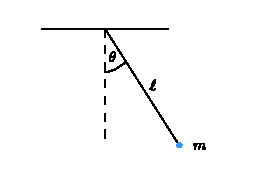
\includegraphics[width=0.5\linewidth]{res/svg/simple_pendulum.drawio}
  \caption{Simple pendulum}
\end{figure}
Now we can discuss the problem of a simple pendulum in the Hamilton formalism. We have a mass $m$ attached to a thin massless rod of length $\ell$. The constraint given by the rod is holonomic and scleronomic:
\begin{equation}
  x^2+y^2-\ell^2 = 0
\end{equation}
We have only one independent coordinate. Let us choose the angle $\theta$. We have that:
\begin{equation}
  \begin{split}
    &x = \ell \cos \theta \implies \dot{x} = - \ell \dot{\theta}\sin \theta \\[8pt]
    &y = \ell \sin \theta \implies \dot{y} = \ell \dot{\theta}\cos \theta
  \end{split}
\end{equation}
The potential is just given by the gravitational potential, which in the reference frame that we fixed is:
\begin{equation}
  V = -mgy = -mg \ell \cos \theta
\end{equation}
The Lagrangian is:
\begin{equation}
  \lagr = \dfrac{1}{2}m\ell^2\dot{\theta}^2 + mg \ell \cos \theta
\end{equation}
The conjugated momenta is:
\begin{equation}
  p_{\theta} = \pdv{\lagr}{\dot{\theta}} = m\ell^2\dot{\theta} = L_z
\end{equation}
And so:
\begin{equation}
  \dot{\theta} = \dfrac{L_z}{m\ell^2}
\end{equation}
The Hamiltonian is:
\begin{equation}
  \hamfun = p_{\theta}\dot{\theta} - \lagr = L_z\dot{\theta} - \dfrac{1}{2}\dfrac{L_z^2}{m\ell^2} - mg \ell \cos \theta = \dfrac{p_{\theta}^2}{2m\ell^2} - mg \ell \cos \theta
\end{equation}
The first \hamiltonref\;gives:
\begin{equation}
  \dot{\theta} = \pdv{\hamfun}{p_{\theta}} = \dfrac{L_z}{m\ell^2}
\end{equation}
Which is already known. The second one gives:
\begin{equation}
  \dot{p}_\theta = -\pdv{\hamfun}{\theta} = - mg \ell \sin \theta
\end{equation}
And so we have:
\begin{equation}
  \begin{split}
    &\dv{}{t}\brackets{m\ell^2\dot{\theta}} = - mg \ell \sin \theta \\[8pt]
    &\boxed{\ddot{\theta} = - \dfrac{g}{\ell} \sin \theta}
  \end{split}
\end{equation}
This is indeed the known equation for the pendulum.\\
\subsection{Ex. 3}
\begin{figure}[H]
  \centering
  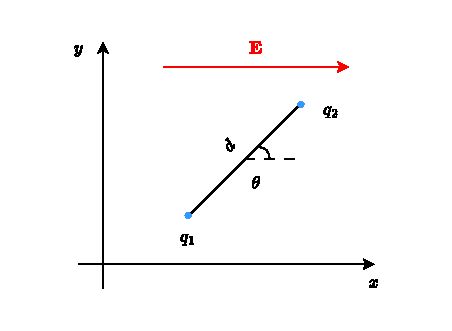
\includegraphics[width=0.5\linewidth]{res/svg/dipole.drawio}
\end{figure}
Now let us take a system made of two charges $q_1$ and $q_2$ of equal mass, with a bar with negligible mass that fixes the distance $d$. Imagine there is an electrostatic field acting on the particles. The motion of the particles is happening on a plane so we have 3 generalized coordinates. We can take the coordinates of the centre of mass $(X, Y)$ and the angle of the bar. We can split the contribution of the kinetic energy with the contribution of the centre of mass and the rotation around the centre of mass:
\begin{equation}
  T = T_{CM} + T' = \dfrac{1}{2}M(\dot{X}^2+\dot{Y}^2) + \dfrac{1}{2}I\dot{\theta}^2
\end{equation}
Now we know $M = 2m$ and $I = 2m\brackets{\dfrac{d}{2}}^2 = \dfrac{1}{2}md^2$. The kinetic energy is thus:
\begin{equation}
  T = m(\dot{X}^2+\dot{Y}^2) + \dfrac{1}{4}md^2\dot{\theta}^2
\end{equation}
Now we could in theory use three different approaches:
\begin{itemize}
  \item Use Lagrange equations
  \item Define a potential and use \eleref
  \item Find the Hamiltonian and use \hamiltonref
\end{itemize}
In this case we use the third method under the assumption that $\vec{E} = (E(x), 0, 0)$. Thus, the electric field is only given by the x component of a potential:
\begin{equation}
  E(x) = -\pdv{\potE}{x}
\end{equation}
The gravitational potential is negligible and so:
\begin{equation}
  V = q_1\potE(x_1) + q_2\potE(x_2)
\end{equation}
Which expressed in terms of the generalized coordinates becomes:
\begin{equation}
  V = q_1\potE \brackets{X - \dfrac{d}{2}\cos\theta} + q_2\potE \brackets{X + \dfrac{d}{2}\cos\theta}
\end{equation}
The Lagrangian is:
\begin{equation}
  \lagr = T - V = m(\dot{X}^2+\dot{Y}^2) + \dfrac{1}{4}md^2\dot{\theta}^2 - q_1\potE \brackets{X - \dfrac{d}{2}\cos\theta} - q_2\potE \brackets{X + \dfrac{d}{2}\cos\theta}
\end{equation}
We should also account for a interaction potential but since the distance is fixed this term would be constant and thus the Lagrangian can be defined without it. The Lagrangian does not depend on time thus:
\begin{equation}
  \pdv{\hamfun}{t} = - \pdv{\lagr}{t} = 0 \implies \dv{\hamfun}{t} = 0
\end{equation}
And so the Hamiltonian is a constant of the motion. Also transformation equations do not depend on time and the potential does not depend on the velocities thus $\hamfun = E$. So the Hamiltonian is the energy and it is conserved. Now we find the conjugated momenta:
\begin{equation}
  \begin{split}
    &p_X = \pdv{\lagr}{\dot{X}} = 2m\dot{X} \\[8pt]
    &p_Y = \pdv{\lagr}{\dot{Y}} = 2m\dot{Y} \\[8pt]
    &p_\theta = \pdv{\lagr}{\dot{\theta}} = \dfrac{1}{2}md^2\dot{\theta} = L_z \\[8pt]
  \end{split}
\end{equation}
The Hamiltonian will be:
\begin{equation}
  \begin{split}
    \hamfun &= 2m\dot{X}^2 + 2m\dot{Y}^2+ \dfrac{1}{2}md^2\dot{\theta}^2 - m(\dot{X}^2+\dot{Y}^2) - \dfrac{1}{4}md^2\dot{\theta}^2 + \\[8pt]
    &+ q_1\potE \brackets{X - \dfrac{d}{2}\cos\theta} + q_2\potE \brackets{X + \dfrac{d}{2}\cos\theta} = \\[8pt]
    &= m\brackets{\dot{X}^2 + \dot{Y}^2} + \dfrac{L_z^2}{md^2} + q_1\potE \brackets{X - \dfrac{d}{2}\cos\theta} + q_2\potE \brackets{X + \dfrac{d}{2}\cos\theta}
  \end{split}
\end{equation}
Now the interesting \hamiltonref\;are the ones who give the $\dot{p}_{\alpha}$ since we already know the $\dot{q}_{\alpha}$ in terms of the momenta from the Lagrangian part. We have that:
\begin{equation}
  \begin{split}
    &\dot{p}_X = -\pdv{\hamfun}{X} = - q_1 \pdv{\potE}{X} - q_2 \pdv{\potE}{X} = q_1E(x_1) + q_2E(x_2) \\[8pt]
    &\dot{p}_Y = -\pdv{\hamfun}{Y} = 0 \\[8pt]
    &\dot{p}_\theta = -\pdv{\hamfun}{\theta} = - q_1 \pdv{\potE}{\theta} - q_2 \pdv{\potE}{\theta} = - q_1 \pdv{\potE}{x_1}\pdv{x_1}{\theta} - q_2 \pdv{\potE}{x_2}\pdv{x_2}{\theta} = \\[8pt]
    &= q_1E(x_1)\dfrac{d}{2}\sin \theta - q_2E(x_2)\dfrac{d}{2}\sin \theta
  \end{split}
\end{equation}
And so $\dot{p}_X$ is the total force and $\dot{p}_{\theta}$ is the total torque. Now consider the case where the two charges are equal but have opposite sign ($q_1 = -q$, $q_2 = q$):
\begin{equation}
  \dot{p}_X = q \brackets{E(x_2) - E(x_1)}\\[8pt]
\end{equation}
If the field is uniform $E(x_2) = E(x_1) = E \implies \vec{F} = 0$, but we still have torque:
\begin{equation}
  \dv{L_z}{t} = -q\dfrac{d}{2}\sin \theta \brackets{E(x_1) + E(x_2)} = -\underbrace{qd}_p E\sin \theta
\end{equation}
And so:
\begin{equation}
  \dv{L_z}{t} = -\brackets{\vec{p} \cross \vec{E}}_z
\end{equation}
Where $\vec{p}$ is the dipole vector.
\subsection{Ex. 4}
\begin{figure}[H]
  \centering
  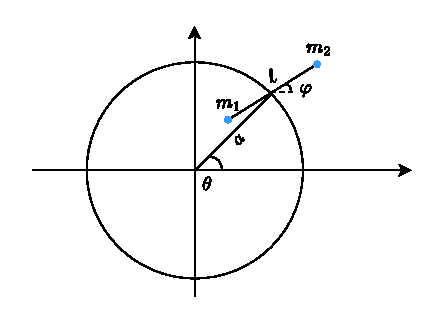
\includegraphics[width=0.7\linewidth]{res/svg/rail_and_bar.drawio}
\end{figure}
A massless bar of length $\ell$ with two bodies $m_1$, $m_2$ is attached in the centre of mass to a system composed of a vertical rail of radius $a$. The system is under the action of the gravitational potential. We have $2$ masses so we start from $3N = 6$ cartesian coordinates, but the motion is constrained on the vertical plane and we also have two constraints which are the bar and the rail so the number of independent coordinates is $n=2$. We can simply use the angles $\theta$ and $\varphi$ to describe the system. The coordiantes of the centre of mass are:
\begin{equation}
  \begin{split}
    X &= a\cos\theta \\[8pt]
    Y &= a\sin\theta
  \end{split}
\end{equation}
If the masses are equal $m_1 = m_2 = m$ then their coordiantes are:
\begin{equation}
  \begin{split}
    &x_1 = X - \dfrac{\ell}{2}\cos\varphi = a\cos\theta - \dfrac{\ell}{2}\cos\varphi \\[8pt]
    &y_1 = Y - \dfrac{\ell}{2}\sin\varphi = a\sin\theta - \dfrac{\ell}{2}\sin\varphi \\[8pt]
    &x_2 = X + \dfrac{\ell}{2}\cos\varphi = a\cos\theta + \dfrac{\ell}{2}\cos\varphi \\[8pt]
    &y_2 = Y + \dfrac{\ell}{2}\sin\varphi = a\sin\theta + \dfrac{\ell}{2}\sin\varphi \\[8pt]
  \end{split}
\end{equation}
The transformation equations do not depend on time so the kinetic energy will be a quadratic function of the velocities. We have that:
\begin{equation}
  \begin{split}
    &\dot{x}_1 = -a\dot{\theta}\sin\theta + \dfrac{\ell}{2}\dot{\varphi}\sin\varphi \\[8pt]
    &\dot{y}_1 = a\dot{\theta}\cos\theta - \dfrac{\ell}{2}\dot{\varphi}\cos\varphi \\[8pt]
    &\dot{x}_2 = -a\dot{\theta}\sin\theta - \dfrac{\ell}{2}\dot{\varphi}\sin\varphi \\[8pt]
    &\dot{y}_2 = a\dot{\theta}\cos\theta + \dfrac{\ell}{2}\dot{\varphi}\cos\varphi \\[8pt]
  \end{split}
\end{equation}
And so the kinetic energy will be:
\begin{equation}
  T = \frac{1}{2}m\left(\dot{x}_1^2 + \dot{y}_1^2 + \dot{x}_2^2 + \dot{y}_2^2\right) = m a^2 \dot{\theta}^2 + \frac{1}{4} m \ell^2 \dot{\varphi}^2
\end{equation}
We could have gotten this just by applying König's theorem:
\begin{equation}
  T = T' + T_{CM} = m a^2 \dot{\theta}^2 + \frac{1}{4} m \ell^2 \dot{\varphi}^2
\end{equation}
The potential is simply:
\begin{equation}
  V = mg\brackets{y_1 + y_2} = mg\brackets{a\sin\theta - \cancel{\dfrac{\ell}{2}\sin\varphi} + a\sin\theta + \cancel{\dfrac{\ell}{2}\sin\varphi}} = 2mga\sin\theta
\end{equation}
And so the Lagrangian is:
\begin{equation}
  \lagr = T - V = m a^2 \dot{\theta}^2 + \frac{1}{4} m \ell^2 \dot{\varphi}^2 - 2mga\sin\theta
\end{equation}
Thus the two conjugate momenta are:
\begin{equation}
  \begin{split}
    p_{\theta} = \pdv{\lagr}{\dot{\theta}} = 2m a^2 \dot{\theta} \\[8pt]
    p_{\varphi} = \pdv{\lagr}{\dot{\varphi}} = \dfrac{1}{2} m \ell^2 \dot{\varphi}
  \end{split}
\end{equation}
We can notice that $p_{\varphi}$ is constant since $\varphi$ is a cyclic coordinate. We can now find the Hamiltonian:
\begin{equation}
  \hamfun = p_{\theta}\dot{\theta} + p_{\varphi}\dot{\varphi} - \lagr = \frac{p_{\theta}^2}{4ma^2} + \frac{p_{\varphi}^2}{m\ell^2} + 2mga\sin\theta
\end{equation}
We only need to solve one Hamilton equation since we already know the relations between the coordinates and the momenta and we also knwo that $\dot{p}_{\varphi} = 0$ so we have:
\begin{equation}
  \dot{p}_{\theta} = -\pdv{\hamfun}{\theta} = -2mga\cos\theta
\end{equation}
The quantity $2mga\cos\theta$ is actually the $z$ component of the torque $\tau_z$ and this means that the system is rotating without a constant angular momentum under the action of gravity, which is what we expect from the setup we have. The equation above also gives us:
\begin{equation}
  \begin{split}
    &2m a^2 \ddot{\theta} = -2mga\cos\theta \\[8pt]
    &\ddot{\theta} + \dfrac{g}{a}\cos\theta = 0
  \end{split}
\end{equation}
\begin{figure}[H]
  \centering
  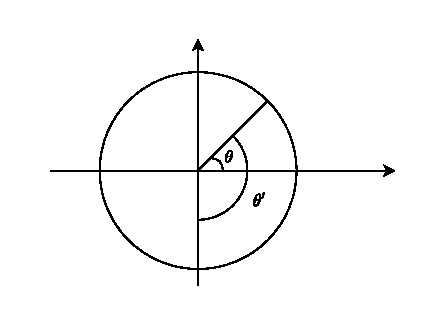
\includegraphics[width=0.5\linewidth]{res/svg/theta_prime.drawio}
\end{figure}
Now if we use the angle $\theta' = \theta + \dfrac{\pi}{2}$ to describe the system we end up with:
\begin{equation}
  \ddot{\theta'} + \dfrac{g}{a}\sin\theta' = 0
\end{equation}
Which is the equation of motion of a pendulum, so the bar is rotating with constant angular momentum around the centre of mass and the centre of mass is moving periodically on the rail.

\chapter{Applications of Lagrange formalism}
In this chapter we will discuss some potential applications of the Lagrange picture of classical mechanics.
\section{Theory of small oscillations}
Many physical problems have an oscillatory nature but, when we try to solve those problems, we usually encounter difficult (sometimes impossible) differential equations.
For this reason we now introduce a systematic way to deal with oscillatory problems in the case of a small oscillation.
\subsection{$\mathbf{n = 1}$ degree of freedom systems}
Let's start with a 1 degree of freedom system. In this case the Lagrangian may look something like this:
\begin{equation}
    \lagr = \dfrac{1}{2}m\dot{q}^2 - V(q)
\end{equation}
Notice that we asked for a potential that only depends on the coordinate $q$.
We take in consideration the system near point of local minimum for the potential.
\begin{figure}[!ht]
    \centering
    \includesvg[width=0.6\textwidth]{res/svg/potential1Dapprox}
    \caption{1-D potential}
    \label{fig:image10}
\end{figure}
Given this we can approximate the potential to it's second order Taylor expansion near the point $q_0$ (local minimum):
\begin{equation}
    V \simeq V(q_0) + \cancel{\pdv{V}{q}\bigg|_{q_0}}(q-q_0) + \dfrac{1}{2}\pdv[2]{V}{q}\bigg|_{q_0}(q-q_0)^2
\end{equation}
The first derivative is zero since we are at a minimum, we can also ignore the value of the potential $V(q_0)$ and set it equal to zero, since we can always change the potential reference. Finally, we define:
\begin{equation}
    \eta \defineeq q-q_0
\end{equation}
And so we get:
\begin{equation} \label{e:potential_1D_oscillation}
    V(\eta) \simeq \dfrac{1}{2}\underbrace{\pdv[2]{V}{\eta}\bigg|_{q_0}}_{\Velegant}\eta^2 = \dfrac{1}{2}\Velegant\eta^2
\end{equation}
Where we defined the second order partial derivative as a known quantity $\Velegant$. We also know that, since $q$ and $\eta$ are different only for a constant term:
\begin{equation} \label{e:kinetic_1D_oscillation}
    T = \dfrac{1}{2}m\dot{q}^2 = \dfrac{1}{2}m\dot{\eta}^2
\end{equation}
From this we can write the \eleref :
\begin{equation}
    \begin{split}
        \dv{}{t}\pdv{\lagr}{\dot{\eta}} -\pdv{\lagr}{\eta} = 0 \\[8pt]
        \dv{}{t}\pdv{T}{\dot{\eta}} + \pdv{V}{\eta} = 0
    \end{split}
\end{equation}
Substituting what we got in \eqref{e:potential_1D_oscillation} and \eqref{e:kinetic_1D_oscillation}:
\begin{equation}
    \begin{split}
        \dv{}{t}(m\dot{\eta}) + \Velegant\eta &= 0\\[8pt]
        m\ddot{\eta} + \Velegant\eta &= 0
    \end{split}
\end{equation}
From which we get this condition:
\begin{equation} \label{e:condition_1D_oscillation}
    \ddot{\eta} =- \dfrac{\Velegant\eta}{m}
\end{equation}
We are searching for solutions of this type:
\begin{equation}
    \eta (t) = a\efunction^{-i\omega t}
\end{equation}
And so we evaluate the second order derivative:
\begin{eqnarray}
    \ddot{\eta} (t) = -a\omega^2\efunction^{-i\omega t}
\end{eqnarray}
We now impose the condition that $a\neq 0$ which is reasonable since $a=0$ would correspond to the absence of motion, so from \eqref{e:condition_1D_oscillation} we get:
\begin{equation}
    \begin{split}
        m\omega^2\cancel{a\efunction^{-i\omega t}} &= \Velegant\cancel{a\efunction^{-i\omega t}}\\[8pt]
        \omega &= \pm \sqrt{\dfrac{\Velegant}{m}}
    \end{split}
\end{equation}
By convention we usually take the $+$ sign and refer to the other solution as $-\omega$. The general solution for $\eta$ will be of this form:
\begin{equation}
    \eta (t) = ca\efunction^{-i\omega t} + c'a\efunction^{i\omega t} = A \sin(\omega t + \varphi) = A \sin\brackets{\sqrt{\dfrac{\Velegant}{m}} t + \varphi}
\end{equation}
\subsection{$\mathbf{n\geq 2}$ degrees of freedom systems}
Now we want to discuss a more general type of system with $n\geq2$ degrees of freedom. Again we take in consideration a point $\vec{q}_0 = (q_{1,0}, q_{2,0}, \,\dots\, ,q_{n,0})$ of local minimum for the potential $V$ which now is a function of all the coordinates $q_{\alpha}$.
\begin{figure}[!ht]
    \centering
    \includesvg[width=0.6\textwidth]{res/svg/potential2Dapprox}
    \caption{2-D potential}
    \label{fig:image11}
\end{figure}
In this case the potential can be approximated near the point with the Taylor formula for multivariable scalar functions:
\begin{equation} \label{e:taylor_potential_scalar_product}
    V(\vec{q}) \simeq \underbrace{V(\vec{q}_0)}_{\text{constant}} + \cancel{\langle \grad V(\vec{q}_0), \vec{q}-\vec{q}_0\rangle} + \dfrac{1}{2}\langle H V(\vec{q}_0)(\vec{q}-\vec{q}_0), (\vec{q}-\vec{q}_0)\rangle
\end{equation}
Again we exploit the fact that we can choose an arbitrary level for the potential, and we define:
\begin{equation}
    \eta_{\alpha} = q_{\alpha} - q_{\alpha,0}
\end{equation}
Expanding \eqref{e:taylor_potential_scalar_product} we get:
\begin{equation}
    \begin{split}
        V(\vec{q}) &\simeq \dfrac{1}{2}\bigsum_{\alpha}\bigsum_{\beta}\dfrac{\partial^2 V}{\partial q_{\alpha} \partial q_{\beta}}\bigg|_{\vec{0}}(q_{\alpha} - q_{\alpha,0})(q_{\beta} - q_{\beta,0})\\[8pt]
        V(\vec{\eta}) &\simeq \dfrac{1}{2}\bigsum_{\alpha}\bigsum_{\beta}\underbrace{\dfrac{\partial^2 V}{\partial \eta_{\alpha} \partial \eta_{\beta}}\bigg|_{\vec{0}}}_{\Velegant_{\alpha \beta} = \Velegant_{\beta \alpha}}\eta_{\alpha}\eta_{\beta}\\[8pt]
        V(\vec{\eta}) &\simeq \dfrac{1}{2}\bigsum_{\alpha}\bigsum_{\beta}\Velegant_{\alpha \beta}\eta_{\alpha}\eta_{\beta}
    \end{split}
\end{equation}
For the kinetic energy $T$ we assume that the transformation equations do not depend on time:
\begin{equation}
    T = \dfrac{1}{2}\bigsum_{\alpha}\bigsum_{\beta}\Telegant'_{\alpha \beta} \dot{\eta}_{\alpha}\dot{\eta}_{\beta}
\end{equation}
We consider the Taylor expansion of $\Telegant'_{\alpha \beta}$. In this case we can stop at the first order because there is no reason to assume that the kinetic energy and the potential energy have a minimum at the same point:
\begin{equation}
    \Telegant'_{\alpha \beta} \simeq \Telegant'_{\alpha \beta}(\vec{0}) + \bigsum_{\gamma}\pdv{\Telegant'_{\alpha \beta}}{\eta_{\gamma}}\bigg|_{\vec{0}}\eta_{\gamma}
\end{equation}
Going back to the general expression for $T$ we get:
\begin{equation}
    \begin{split}
        T &\simeq \dfrac{1}{2}\bigsum_{\alpha}\bigsum_{\beta}\brackets{\Telegant'_{\alpha \beta}(\vec{0}) + \bigsum_{\gamma}\pdv{\Telegant'_{\alpha \beta}}{\eta_{\gamma}}\bigg|_{\vec{0}}\eta_{\gamma}} \dot{\eta}_{\alpha}\dot{\eta}_{\beta} =\\[8pt]
        &= \dfrac{1}{2}\bigsum_{\alpha}\bigsum_{\beta}\bigsum_{\gamma}\underbrace{\pdv{\Telegant'_{\alpha \beta}}{\eta_{\gamma}}\bigg|_{\vec{0}}\eta_{\gamma} \dot{\eta}_{\alpha}\dot{\eta}_{\beta}}_{o(\eta \dot{\eta}^2)} + \dfrac{1}{2}\bigsum_{\alpha}\bigsum_{\beta}\underbrace{\Telegant'_{\alpha \beta}(\vec{0})\dot{\eta}_{\alpha}\dot{\eta}_{\beta}}_{o(\dot{\eta}^2)}
    \end{split}
\end{equation}
We can neglect the first term since it is small with respect to the second term. Now we define:
\begin{equation}
    \Telegant_{\alpha \beta} \defineeq \Telegant'_{\alpha \beta}(\vec{0})
\end{equation}
Those are just numbers which correspond to the value of the kinetic energy at the origin. We can put those numbers into a matrix:
\begin{equation}
    \hat{\Telegant}=
    \begin{pmatrix}
        \Telegant_{1 1} & \Telegant_{1 2} &  \,\dots\,  & \Telegant_{1 n}\\[8pt]
        \Telegant_{2 1} & \Telegant_{2 2} &  \,\dots\,  &  \,\dots\, \\[8pt]
         \,\dots\,  &  \,\dots\,  &  \,\dots\,  &  \,\dots\, \\[8pt]
        \Telegant_{n 1} &  \,\dots\,  &  \,\dots\,  & \Telegant_{n n}\\[8pt]
    \end{pmatrix}
\end{equation}
Similarly we can put the values of $\Velegant_{\alpha \beta}$ into a matrix:
\begin{equation}
    \hat{\Velegant}=
    \begin{pmatrix}
        \Velegant_{1 1} & \Velegant_{1 2} &  \,\dots\,  & \Velegant_{1 n}\\[8pt]
        \Velegant_{2 1} & \Velegant_{2 2} &  \,\dots\,  &  \,\dots\, \\[8pt]
         \,\dots\,  &  \,\dots\,  &  \,\dots\,  &  \,\dots\, \\[8pt]
        \Velegant_{n 1} &  \,\dots\,  &  \,\dots\,  & \Velegant_{n n}\\[8pt]
    \end{pmatrix}
\end{equation}
Also we have that:
\begin{equation}
    \dfrac{1}{2}\bigsum_{\alpha}\bigsum_{\beta}\Telegant_{\alpha \beta}\dot{\eta}_{\alpha}\dot{\eta}_{\beta}
\end{equation}
So the Lagrangian for the system is:
\begin{equation}
    \lagr = \dfrac{1}{2}\bigsum_{\alpha}\bigsum_{\beta}\brackets{\Telegant_{\alpha \beta}\dot{\eta}_{\alpha}\dot{\eta}_{\beta} - \Velegant_{\alpha \beta}\eta_{\alpha}\eta_{\beta}}
\end{equation}
The terms of the \eleref\;are:
\begin{equation}
    \begin{split}
        \pdv{\lagr}{\eta_{\gamma}} &= -\pdv{V}{\eta_{\gamma}} = -\dfrac{1}{2}\bigsum_{\alpha}\bigsum_{\beta}\Velegant_{\alpha \beta} \pdv{}{\eta_{\gamma}}\brackets{\eta_{\alpha}\eta_{\beta}}\\[8pt]
        \pdv{\lagr}{\dot{\eta}_{\gamma}} &= \pdv{T}{\dot{\eta}_{\gamma}} = \dfrac{1}{2}\bigsum_{\alpha}\bigsum_{\beta}\Telegant_{\alpha \beta}\pdv{}{\dot{\eta}_{\gamma}}\brackets{\dot{\eta}_{\alpha}\dot{\eta}_{\beta}}
    \end{split}
\end{equation}
Evaluating the partial derivatives we get:
\begin{equation}
    \begin{split}
        \pdv{\lagr}{\eta_{\gamma}} &= -\dfrac{1}{2}\bigsum_{\alpha}\bigsum_{\beta}\Velegant_{\alpha \beta} \bbrackets{\eta_{\beta}\underbrace{\pdv{\eta_{\alpha}}{\eta_{\gamma}}}_{\delta_{\gamma \alpha}} + \eta_{\alpha}\underbrace{\pdv{\eta_{\beta}}{\eta_{\gamma}}}_{\delta_{\gamma \beta}}} =\\[8pt]
        &= -\dfrac{1}{2}\bigsum_{\alpha}\bigsum_{\beta}\Velegant_{\alpha \beta} \eta_{\beta}\delta_{\gamma \alpha} - \dfrac{1}{2}\bigsum_{\alpha}\bigsum_{\beta}\Velegant_{\alpha \beta} \eta_{\alpha}\delta_{\gamma \beta} = \\[8pt]
        &= -\dfrac{1}{2}\bigsum_{\beta}\Velegant_{\gamma \beta} \eta_{\beta} - \dfrac{1}{2}\bigsum_{\alpha}\Velegant_{\alpha \gamma} \eta_{\alpha} =\\[8pt]
        &= -\bigsum_{\alpha}\Velegant_{\alpha \gamma} \eta_{\alpha}
    \end{split}
\end{equation}
We simplified the summation in the second line because of the Kronecker delta, and we can notice that in the third line the two terms are actually identical due to the fact that $\Velegant_{\alpha \gamma} = \Velegant_{\gamma \beta}$ and we are summing over all indices. The calculation for the kinetic energy is the same, and we get:
\begin{equation}
    \pdv{\lagr}{\dot{\eta}_{\gamma}} = \bigsum_{\alpha}\Telegant_{\alpha \gamma} \dot{\eta}_{\alpha}
\end{equation}
Hence we evaluate the total time derivative:
\begin{equation}
    \dv{}{t}\pdv{\lagr}{\dot{\eta}_{\gamma}} = \dv{}{t}\bigsum_{\alpha}\Telegant_{\alpha \gamma} \eta_{\alpha} = \bigsum_{\alpha}\Telegant_{\alpha \gamma} \ddot{\eta}_{\alpha}
\end{equation}
So the \eleref\;are:
\begin{equation} \label{e:ele_for_gamma}
    \bigsum_{\alpha}\brackets{\Telegant_{\alpha \gamma} \ddot{\eta}_{\alpha} + \Velegant_{\alpha \gamma} \eta_{\alpha}} = 0
\end{equation}
for all the possible $\gamma$.\\
Taking into account the fact that we look for solutions like:
\begin{equation}
    \eta_{\alpha} (t) = a_{\alpha}\efunction^{-i\omega t}
\end{equation}
\textbf{N.B.} The coefficients $a_{\alpha}$ may be complex numbers.\\
Substituting into \eqref{e:ele_for_gamma} we get:
\begin{equation} \label{e:eigenvalue_alpha}
    \begin{split}
        \bigsum_{\alpha}\brackets{-\omega^2\Telegant_{\alpha \gamma} a_{\alpha}\cancel{\efunction^{-i\omega t}} + \Velegant_{\alpha \gamma}a_{\alpha}\cancel{\efunction^{-i\omega t}}} &= 0\\[8pt]
        \bigsum_{\alpha}\brackets{-\omega^2\Telegant_{\alpha \gamma} + \Velegant_{\alpha \gamma}}a_{\alpha} &= 0
    \end{split}
\end{equation}
This is true for any $\gamma$ so we are obtaining a set of \textit{homogeneous first order equations}. We know from linear algebra that the only way for this system to allow solutions different from the trivial solution is to ask for at least one equation to be a linear combination of the others.
In other terms we want the determinant of the coefficient matrix to be zero. We can now express the system as follows:
\begin{equation}
    \brackets{-\omega^2\hat{\Telegant} + \hat{\Velegant}}\vec{a} = \vec{0}
\end{equation}
Let $\lambda = \omega^2$:
\begin{equation}
    \boxed{\hat{\Velegant}\vec{a} = \lambda\hat{\Telegant}\vec{a}}
\end{equation}
This equation is called \textbf{generalized eigenvalue equation}. In fact if we have $\hat{\Telegant} = \mathbb{I}$ we return to the ``regular'' eigenvalue equation. In order to find the coefficients $\lambda$ we must solve this equation:
\begin{equation}
    \det(\hat{\Velegant}-\lambda\hat{\Telegant}) = 0
\end{equation}
This is an $n$ degree polynomial with $n$ solutions $\lambda_i$ with $i=1,2, \,\dots\, ,n$. The solutions satisfy some properties:
\begin{itemize}
    \item $\lambda_i \in \mathbb{R}$
    \item $\lambda_i > 0$
\end{itemize}
This means that $\omega_i = \pm \sqrt{\lambda_i}$ is real for any $i$. Putting $\lambda_i$ back into \eqref{e:eigenvalue_alpha} we get an expression depending on $\gamma$, thus we have a system of equations:
\begin{equation}
    \begin{cases}
        \bigsum_{\alpha}\brackets{-\lambda_i\Telegant_{\alpha 1} + \Velegant_{\alpha 1}}a_{\alpha}^{(i)} &= 0\\[10pt]
        \bigsum_{\alpha}\brackets{-\lambda_i\Telegant_{\alpha 2} + \Velegant_{\alpha 2}}a_{\alpha}^{(i)} &= 0\\[10pt]
         \,\dots\, \\[10pt]
        \bigsum_{\alpha}\brackets{-\lambda_i\Telegant_{\alpha n} + \Velegant_{\alpha n}}a_{\alpha}^{(i)} &= 0
    \end{cases}
\end{equation}
In this system at least one equation is linearly dependent on the others since we asked that the determinant of the coefficient matrix is zero. In this way we can find all the components of the vector $\vec{a}^{(i)}$, which is called \textbf{generalized eigenvector}.
Those vectors must satisfy a condition:
\begin{equation}
    [\vec{a}^{(i)}]^{\dagger}\;\hat{\Telegant}\;[\vec{a}^{(j)}] = 0
\end{equation}
This condition is called $\hat{\Telegant}$-orthogonality and is a generalization of the concept of orthogonality. In fact this condition reduces to the ``usual'' case if $\hat{\Telegant} = \mathbb{I}$ and the vectors are real valued:
\begin{equation}
    \begin{split}
        [\vec{a}^{(i)}]^{\dagger}\;\mathbb{I}\;[\vec{a}^{(j)}] &= 0\\[8pt]
        \transpose{[\vec{a}^{(i)}]} [\vec{a}^{(j)}] &= 0 \\[8pt]
        \vec{a}^{(i)}\cdot \vec{a}^{(j)} &= 0
    \end{split}
\end{equation}
We also want to normalize the vectors. Again the concept of normalization is generalized as follows:
\begin{equation}
    [\vec{a}^{(i)}]^{\dagger}\;\hat{\Telegant}\;[\vec{a}^{(i)}] = 1
\end{equation}
A solution to the system is:
\begin{equation}
    \vec{\eta} = \begin{pmatrix}
        \eta_1\\[8pt]
        \eta_2\\[8pt]
         \,\dots\, \\[8pt]
        \eta_n
    \end{pmatrix}
    =
    \begin{pmatrix}
        a_1\\[8pt]
        a_2\\[8pt]
         \,\dots\, \\[8pt]
        a_n
    \end{pmatrix}\efunction^{-i\omega t}
\end{equation}
Actually a more general solution is given by a linear combination of this solution:
\begin{equation}
    \begin{split}
        \vec{\eta} &= \bigsum_i\brackets{c_i \vec{a}^{(i)} \efunction^{-i\omega_i t} + c_i' \vec{a}^{(i)} \efunction^{i\omega_i t}} =\\[8pt]
        &= \bigsum_i \underbrace{\brackets{c_i \efunction^{-i\omega_i t} + c_i' \efunction^{i\omega_i t}}}_{\text{components of $\vec{\eta}$ along $\vec{a}^{(i)}$}}\vec{a}^{(i)}
    \end{split}
\end{equation}
For each component we have:
\begin{equation}
    \begin{split}
        \eta_{\alpha} &= \bigsum_i \brackets{c_i \efunction^{-i\omega_i t} + c_i' \efunction^{i\omega_i t}}a_{\alpha}^{(i)} =\\[8pt]
        &=  \underbrace{\bigsum_i A_i \sin(\omega_i t + \varphi_i)}_{\text{non monochromatic}}
    \end{split}
\end{equation}
The terms $\omega_i$ are called \textbf{normal mode frequencies}, and generally they are all different.\\
It is possible to express the solutions as pure harmonic motions (monochromatic) if one uses the eigenvectors as basis vectors. We can also notice that both $\hat{\Velegant}$ and $\hat{\Telegant}$ are diagonalized by the eigenvectors $\vec{a}^{(i)}$.
In this base solution is in the form:
\begin{equation}
    u_i = A_i \sin(\omega_i t + \varphi_i)
\end{equation}
Which indeed is monochromatic. Writing the \eleref\;in this basis we have:
\begin{equation}
    \ddot{u}_i +\lambda_i u_i = 0 \;\;\forall i=1, \,\dots\, ,n
\end{equation}
\subsection{2-D systems. General example}
Let's assume we are dealing with a two-dimensional system with a minimum for the potential at $(q_{10},q_{20})$. Also assume that the kinetic energy taxes the form of:
\begin{equation}
    \hat{\Telegant} = m\begin{pmatrix}
        1 & 0\\[8pt]
        0 & 1
    \end{pmatrix} \Rightarrow \Telegant_{\alpha \beta} = m\delta_{\alpha \beta}
\end{equation}
Expanding the potential in terms of $\eta_1 = q_1-q_{10}$ and $\eta_2 = q_2-q_{20}$ gives:
\begin{equation}
    \begin{split}
        V &\simeq \dfrac{1}{2}\bigsum_{\alpha}\bigsum_{\beta}\brackets{\dfrac{\partial^2 V}{\partial \eta_{\alpha} \partial \eta_{\beta}}\bigg|_{(0,0)}\eta_{\alpha}\eta_{\beta}} =\\[8pt]
        &= \dfrac{1}{2}(\Velegant_{11}\eta_1^2 + \Velegant_{22}\eta_2^2 + \underbrace{\Velegant_{12}\eta_1\eta_2 + \Velegant_{21}\eta_2\eta_1}_{\text{same term}}) =\\[8pt]
        &= \dfrac{1}{2}(\Velegant_{11}\eta_1^2 + \Velegant_{22}\eta_2^2 + 2\Velegant_{12}\eta_1\eta_2 )
    \end{split}
\end{equation}
The kinetic energy instead becomes:
\begin{equation}
    \begin{split}
        T &= \dfrac{1}{2}\bigsum_{\alpha}\bigsum_{\beta}m \delta_{\alpha \beta} \dot{\eta}_{\alpha}\dot{\eta}_{\beta} =\\[8pt]
        &= \dfrac{1}{2}m(\dot{\eta}_1^2 + \dot{\eta}_2^2)
    \end{split}
\end{equation}
The Lagrangian then becomes:
\begin{equation}
    \lagr = \dfrac{1}{2}m(\dot{\eta}_1^2 + \dot{\eta}_2^2) - \dfrac{1}{2}(\Velegant_{11}\eta_1^2 + \Velegant_{22}\eta_2^2 + 2\Velegant_{12}\eta_1\eta_2 )
\end{equation}
Let us divide the Lagrangian by $m$ and define:
\begin{equation}
    \lagr' = \dfrac{1}{m}\lagr
\end{equation}
\begin{equation}
    \hat{\Telegant}' = \dfrac{1}{m}\hat{\Telegant} = \begin{pmatrix}
        1 & 0\\[8pt]
        0 & 1
    \end{pmatrix}
\end{equation}
\begin{equation}
    \hat{\Velegant}' = \dfrac{1}{m}\hat{\Velegant} = \begin{pmatrix}
        \dfrac{\Velegant_{11}}{m} & \dfrac{\Velegant_{12}}{m}\\[8pt]
        \dfrac{\Velegant_{21}}{m} & \dfrac{\Velegant_{22}}{m}
    \end{pmatrix} = \begin{pmatrix}
        \Velegant_{11}' & \Velegant_{12}'\\[8pt]
        \Velegant_{21}' & \Velegant_{22}'
    \end{pmatrix}
\end{equation}
The new Lagrangian becomes:
\begin{equation}
    \lagr' = \dfrac{1}{2}\transpose{\dvec{\eta}} \dvec{\eta} - \dfrac{1}{2}\transpose{\vec{\eta}} \Velegant' \vec{\eta}
\end{equation}
From \eleref\;we get two equations:
\begin{equation}
    \begin{cases}
        \ddot{\eta}_1 + \Velegant'_{11}\eta_1 + \Velegant'_{12}\eta_2 = 0\\[8pt]
        \ddot{\eta}_2 + \Velegant'_{22}\eta_2 + \Velegant'_{12}\eta_1 = 0
    \end{cases} \bigg|\;\text{coupled equations}
\end{equation}
Now impose that the solutions are in the form:
\begin{equation}
    \begin{split}
        \eta_1 = a_1\efunction^{-i\omega t} \\[8pt]
        \eta_2 = a_2\efunction^{-i\omega t}
    \end{split}
\end{equation}
The system becomes:
\begin{equation}
    \begin{cases}
        -\omega^2 a_1 + \Velegant'_{11}a_1 + \Velegant'_{12}a_2 = 0\\[8pt]
        \Velegant'_{12}a_1 -\omega^2 a_2 + \Velegant'_{22}a_2 = 0
    \end{cases}
\end{equation}
In this case the generalized eigenvalue equation reduces to the usual case, and we get the two solutions $\lambda_1$ and $\lambda_2$. Substituting $\lambda_1$ into the eigenvalue equation we get:
\begin{equation}
    \begin{cases}
        \brackets{\Velegant'_{11}-\lambda_1}a_1^{(1)} + \Velegant'_{12}a_2^{(1)} = 0\\[8pt]
        \Velegant'_{12}a_1^{(1)} + \brackets{\Velegant'_{22}-\lambda_1}a_2^{(1)} = 0
    \end{cases}
\end{equation}
One of the two equation must depend on the other. Since we have two equations we can arbitrarily pick one and get the relation between the coefficients:
\begin{equation}
    a_2^{(1)} = a_1^{(1)}\dfrac{\lambda_1 - \Velegant'_{11}}{\Velegant'_{12}}
\end{equation}
And so we have:
\begin{equation}
    \vec{a}^{\;(1)} = a_1^{(1)}\begin{pmatrix}
        1 \\[8pt] \dfrac{\lambda_1 - \Velegant'_{11}}{\Velegant'_{12}}
    \end{pmatrix}
\end{equation}
Similarly for $\lambda_2$ we get:
\begin{equation}
    \vec{a}^{\;(2)} = a_1^{(2)}\begin{pmatrix}
        1 \\[8pt] \dfrac{\lambda_2 - \Velegant'_{11}}{\Velegant'_{12}}
    \end{pmatrix}
\end{equation}
Now let's define:
\begin{equation}
    \begin{split}
        K_1\;\text{s.t.}\; a^{(1)} = K_1\Velegant'_{12}\\[8pt]
        K_2\;\text{s.t.}\; a^{(2)} = K_2\Velegant'_{12}
    \end{split}
\end{equation}
And the vectors can be rewritten as:
\begin{equation}
    \begin{split}
        \vec{a}^{\;(1)} = K_1\begin{pmatrix}
            \Velegant'_{12} \\[8pt] \lambda_1 - \Velegant'_{11}
        \end{pmatrix}\\[8pt]
        \vec{a}^{\;(2)} = K_2\begin{pmatrix}
            \Velegant'_{12} \\[8pt] \lambda_2 - \Velegant'_{11}
        \end{pmatrix}
    \end{split}
\end{equation}
The most general solution is a linear combination of all the single solutions:
\begin{equation}
    \vec{\eta} = \begin{pmatrix}
        c_1 a_1^{(1)}\efunction^{-i\omega_1 t} + c_1' a_1^{(1)}\efunction^{i\omega_1 t} + c_2 a_1^{(2)}\efunction^{-i\omega_2 t} + c_2' a_1^{(2)}\efunction^{i\omega_2 t}\\[8pt]
        c_1 a_2^{(1)}\efunction^{-i\omega_1 t} + c_1' a_2^{(1)}\efunction^{i\omega_1 t} + c_2 a_2^{(2)}\efunction^{-i\omega_2 t} + c_2' a_2^{(2)}\efunction^{i\omega_2 t}
    \end{pmatrix}
\end{equation}
Substituting the components of the vectors $\vec{a}$:
\begin{equation}
    \begin{split}
        \vec{\eta} = \begin{pmatrix}
            c_1 K_1\Velegant'_{12}\efunction^{-i\omega_1 t} + c_1' K_1\Velegant'_{12}\efunction^{i\omega_1 t} +  \,\dots\, \\[8pt]
            c_1 K_1\Velegant'_{12}\efunction^{-i\omega_1 t} + c_1' K_1\Velegant'_{12}\efunction^{i\omega_1 t} +  \,\dots\,
        \end{pmatrix}\\[8pt]
        \vec{\eta} = \begin{pmatrix}
            A_1 \sin(\omega_1 t + \varphi_1) + A_2 \sin(\omega_2 t + \varphi_2)\\[8pt]
            A_1 \sin(\omega_1 t + \varphi_1) + A_2 \sin(\omega_2 t + \varphi_2)
        \end{pmatrix}
    \end{split}
\end{equation}
But if we change basis we get:
\begin{equation}
    \vec{\eta} = u_1 \vec{a}^{\;(1)} + u_2 \vec{a}^{\;(2)}
\end{equation}
Where:
\begin{equation}
    \begin{split}
        u_1 = A_1 \sin(\omega_1 t + \varphi_1)\\[8pt]
        u_2 = A_2 \sin(\omega_2 t + \varphi_2)
    \end{split}
\end{equation}
Which are monochromatic signals. Also in this new basis we have:
\begin{equation}
    \begin{split}
        \hat{\Telegant}' = \begin{pmatrix}
            1 & 0\\[8pt]
            0 & 1
        \end{pmatrix}\\[8pt]
        \hat{\Velegant}' = \begin{pmatrix}
            \lambda_1 & 0\\[8pt]
            0 & \lambda_2
        \end{pmatrix}
    \end{split}
\end{equation}
And so the \eleref\;become:
\begin{equation}
    \begin{cases}
        \ddot{u}_1+\lambda_1 u_1 = 0\\[8pt]
        \ddot{u}_2+\lambda_2 u_2 = 0
    \end{cases}
\end{equation}
Those are not coupled equations, and so they can be solved separately.


\subsection{2-D systems. Coupled pendulums}
Now let's take a particular system composed of two ideal pendulums in which the masses are attached by a spring as shown:
\begin{figure}[!ht]
    \centering
    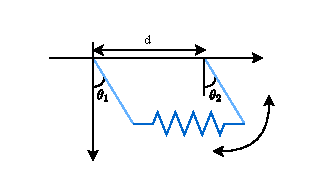
\includegraphics[width=0.6\textwidth]{res/svg/couple_pendulum_1.drawio}
    \caption{Coupled pendulums}
\end{figure}
The rest length of the spring is $d$. Since we have two particles, in principle we have at least $N=3\cdot2=6$ coordinates. Two coordinates can be neglected because the motion only occurs in the $xy$-plane.
The two ropes are a constraint on the position of the particles. In particular both constraints are holomonic and sclermonic:
\begin{equation}
    \begin{cases}
        x_1^2 + y_1^2 = l & \text{(first rope)}\\[8pt]
        (x_2-d)^2 + y_2^2 = l & \text{(second rope)}
    \end{cases}
\end{equation}
We can write the transformation equations as follows:
\begin{equation}
    \begin{cases}
        x_1 = l\sin\theta_1\\[8pt]
        y_1 = -l\cos\theta_1
    \end{cases}\;\;
    \begin{cases}
        x_2 = l\sin\theta_2+d\\[8pt]
        y_2 = -l\cos\theta_2
    \end{cases}
\end{equation}
Since transformation equations do not depend on time the kinetic energy will be a quadratic function of the velocities:
\begin{equation}
    \begin{split}
        T &= \dfrac{1}{2}m(\underbrace{\dot{x}_1^2+\dot{y}_1^2}_{(l\dot{\theta}_1)^2}) + \dfrac{1}{2}m(\underbrace{\dot{x}_2^2+\dot{y}_2^2}_{(l\dot{\theta}_2)^2}) \\[8pt]
        &= \dfrac{1}{2}ml^2(\dot{\theta}_1^2+\dot{\theta}_2^2)
    \end{split}
\end{equation}
We can express this in a matrix form as:
\begin{equation}
    \begin{split}
        T &= \dfrac{1}{2}(\dot{\theta}_1 \dot{\theta}_2)\hat{\Telegant}\begin{pmatrix}
            \dot{\theta}_1 \\[8pt]\dot{\theta}_2
        \end{pmatrix} = \\[8pt]
        &= \dfrac{1}{2}(\dot{\theta}_1 \dot{\theta}_2)ml^2\begin{pmatrix}
            1 & 0\\[8pt]
            0 & 1
        \end{pmatrix}
        \begin{pmatrix}
            \dot{\theta}_1 \\[8pt]\dot{\theta}_2
        \end{pmatrix} = \\[8pt]
    \end{split}
\end{equation}
The potential is the sum of the gravitational potentials of the masses and of the elastic potential of the spring:
\begin{equation}
    \begin{split}
        V &= \underbrace{mgy_1 + mgy_2}_{-mgl(\cos\theta_1+\cos\theta_1)} + \dfrac{1}{2}k\left[\sqrt{(x_2-x_1)^2+(y_2-y_1)^2}-d\right]^2\\[8pt]
        &= -mgl(\cos\theta_1+\cos\theta_1) +\\[8pt]
        &+ \dfrac{1}{2}k\left[\sqrt{(l\sin\theta_2+d-l\sin\theta_1)^2+(l\cos\theta_1-l\cos\theta_2)^2}-d\right]^2\\[8pt]
    \end{split}
\end{equation}
To find the minimum value of the potential we should theoretically evaluate the gradient and solve for $\grad V = \vec{0}$, but if we look at the configuration we can easily notice that the potential is minimum when the pendulums are in the vertical position and the spring is at rest as shown:
\begin{figure}[H]
    \centering
    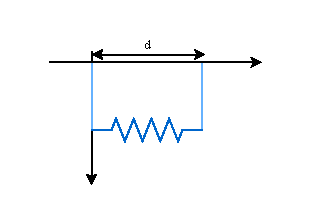
\includegraphics[width=0.6\textwidth]{res/svg/couple_pendulum_still.drawio}
\end{figure}
Thus we can expand the potential at $(0,0)$. Notice that the coordinates $\eta_1$ and $\eta_2$ in this case are equivalent to the ones we chose:
\begin{equation}
    \begin{split}
        V &\simeq V(0,0) +\dfrac{1}{2}\bigsum_{\alpha}\bigsum_{\beta} \dfrac{\partial^2 V}{\partial \theta_{\alpha} \partial \theta_{\beta}}\bigg|_{(0,0)}\theta_{\alpha}\theta_{\beta} = \\[8pt]
        &= V(0,0) +\dfrac{1}{2}\brackets{\Velegant_{11}\theta_1^2 + \Velegant_{22}\theta_2^2 + 2\Velegant_{12}\theta_1\theta_2}
    \end{split}
\end{equation}
This can be expressed in matrix form:
\begin{equation}
    \begin{split}
        V &= \dfrac{1}{2}(\theta_1\;\theta_2)\hat{\Velegant}\begin{pmatrix}
            \theta_1 \\[8pt]
            \theta_2
        \end{pmatrix}\\[8pt]
        V &= \dfrac{1}{2}(\theta_1\;\theta_2)\begin{pmatrix}
            \Velegant_{11} & \Velegant_{12}\\[8pt]
            \Velegant_{12} & \Velegant_{22}
        \end{pmatrix} \begin{pmatrix}
            \theta_1 \\[8pt]
            \theta_2
        \end{pmatrix}
    \end{split}
\end{equation}
If we evaluate all the partial derivatives we get that the matrix $\hat{\Velegant}$ is:
\begin{equation}
    \hat{\Velegant} = \begin{pmatrix}
        mgl+kl^2 & -kl^2\\[8pt]
        -kl^2 & mgl+kl^2
    \end{pmatrix}
\end{equation}
The Lagrangian finally looks like this:
\begin{equation}
    \lagr = \dfrac{1}{2}ml^2(\dot{\theta}_1^2+\dot{\theta}_2^2) - \dfrac{1}{2}\left[(mgl+kl^2)\theta_1^2 + 2(-kl^2)\theta_1\theta_2 + (mgl+kl^2)\theta_2^2 \right]
\end{equation}
And the \eleref\;are:
\begin{equation}
    \begin{cases}
        ml^2\ddot{\theta}_1 + (mgl + kl^2)\theta_1 - kl^2\theta_2 = 0\\[8pt]
        ml^2\ddot{\theta}_2 + (mgl + kl^2)\theta_2 - kl^2\theta_1 = 0
    \end{cases}
\end{equation}
Dividing by $ml^2$ we get:
\begin{equation} \label{e:ode_system_double_pendulum}
    \begin{cases}
        \ddot{\theta}_1 + \brackets{\dfrac{g}{l} + \dfrac{k}{m}}\theta_1 - \dfrac{k}{m}\theta_2 = 0\\[8pt]
        \ddot{\theta}_2 + \brackets{\dfrac{g}{l} + \dfrac{k}{m}}\theta_2 - \dfrac{k}{m}\theta_1 = 0
    \end{cases}
\end{equation}
And so we define a new matrix for the potential:
\begin{equation}
    \hat{\Velegant}' = \dfrac{\hat{\Velegant}}{ml^2}\begin{pmatrix}
        \dfrac{g}{l} + \dfrac{k}{m} & - \dfrac{k}{m}\\[10pt]
        - \dfrac{k}{m} & \dfrac{g}{l} + \dfrac{k}{m}
    \end{pmatrix}
\end{equation}
and for the kinetic energy:
\begin{equation}
    \hat{\Telegant}' = \dfrac{\hat{\Telegant}}{ml^2}\begin{pmatrix}
        1 & 0\\[8pt]
        0 & 1
    \end{pmatrix}
\end{equation}
To find the eigenvalues we need to solve:
\begin{equation}
    \det(\hat{\Velegant}'-\lambda\mathbb{I}) = 0
\end{equation}
From which we get:
\begin{equation}
    \begin{split}
        \begin{vmatrix}
            \dfrac{g}{l} + \dfrac{k}{m} - \lambda & - \dfrac{k}{m}\\[10pt]
            - \dfrac{k}{m} & \dfrac{g}{l} + \dfrac{k}{m} - \lambda
        \end{vmatrix} &= 0\\[8pt]
        \brackets{\dfrac{g}{l} + \dfrac{k}{m} - \lambda}^2 -\brackets{\dfrac{k}{m}}^2 & = 0\\[8pt]
        \brackets{\dfrac{g}{l} + \cancel{\dfrac{k}{m}} - \lambda-\cancel{\dfrac{k}{m}}}\brackets{\dfrac{g}{l} + \dfrac{k}{m} - \lambda+\dfrac{k}{m}} &=0\\[8pt]
        \brackets{\dfrac{g}{l} - \lambda}\brackets{\dfrac{g}{l} + 2\dfrac{k}{m} - \lambda} &=0
    \end{split}
\end{equation}
So we get the values for $\lambda_1$ and $\lambda_2$:
\begin{equation}
    \begin{split}
        \lambda_1 &= \dfrac{g}{l}\\
        \lambda_2 &= \dfrac{g}{l} + 2\dfrac{k}{m}
    \end{split}
\end{equation}
We want solutions like $\theta_i = a_i\efunction^{-i\omega t}$. Substituting this into \eqref{e:ode_system_double_pendulum} we get:
\begin{equation}
    \begin{cases}
        -\omega^2 a_1 \efunction^{-i\omega t} + \brackets{\dfrac{g}{l} + \dfrac{k}{m}} a_1 \efunction^{-i\omega t} - \dfrac{k}{m} a_2 \efunction^{-i\omega t} = 0\\[8pt]
        -\omega^2 a_2 \efunction^{-i\omega t} + \brackets{\dfrac{g}{l} + \dfrac{k}{m}} a_2 \efunction^{-i\omega t} - \dfrac{k}{m} a_1 \efunction^{-i\omega t} = 0
    \end{cases}
\end{equation}
Dividing by $\efunction^{-i\omega t}$ and remembering that $\omega^2 = \lambda$ we get:
\begin{equation}
    \begin{cases}
        \brackets{\dfrac{g}{l} + \dfrac{k}{m} - \lambda} a_1 - \dfrac{k}{m} a_2 = 0\\[8pt]
        -\dfrac{k}{m} a_1 + \brackets{\dfrac{g}{l} + \dfrac{k}{m} - \lambda} a_2 = 0
    \end{cases}
\end{equation}
Substituting $\lambda_1$ gives the eigenvector:
\begin{equation}
    \begin{cases}
        \brackets{\dfrac{g}{l} + \dfrac{k}{m} - \dfrac{g}{l}} a_1 - \dfrac{k}{m} a_2 = 0\\[8pt]
        -\dfrac{k}{m} a_1 + \brackets{\dfrac{g}{l} + \dfrac{k}{m} - \dfrac{g}{l}} a_2 = 0
    \end{cases}
\end{equation}
Simplifying, we get:
\begin{equation}
    \begin{cases}
        \dfrac{k}{m} a_1 - \dfrac{k}{m} a_2 = 0\\[8pt]
        -\dfrac{k}{m} a_1 + \dfrac{k}{m} a_2 = 0
    \end{cases}
\end{equation}
This implies:
\begin{equation}
    a_1 = a_2
\end{equation}
So the eigenvector corresponding to $\lambda_1$ is:
\begin{equation}
    \vec{a}^{\;(1)} = \begin{pmatrix}
        1\\
        1
    \end{pmatrix}
\end{equation}
Substituting $\lambda_2$ gives the eigenvector:
\begin{equation}
    \begin{cases}
        \brackets{\dfrac{g}{l} + \dfrac{k}{m} - \dfrac{g}{l} - 2\dfrac{k}{m}} a_1 - \dfrac{k}{m} a_2 = 0\\[8pt]
        -\dfrac{k}{m} a_1 + \brackets{\dfrac{g}{l} + \dfrac{k}{m} - \dfrac{g}{l} - 2\dfrac{k}{m}} a_2 = 0
    \end{cases}
\end{equation}
Simplifying, we get:
\begin{equation}
    \begin{cases}
        -\dfrac{k}{m} a_1 - \dfrac{k}{m} a_2 = 0\\[8pt]
        -\dfrac{k}{m} a_1 - \dfrac{k}{m} a_2 = 0
    \end{cases}
\end{equation}
This implies:
\begin{equation}
    a_1 = -a_2
\end{equation}
So the eigenvector corresponding to $\lambda_2$ is:
\begin{equation}
    \vec{a}^{\;(2)} = \begin{pmatrix}
        1\\[8pt]
        -1
    \end{pmatrix}
\end{equation}
Any other vector which is a multiple of those vectors is an eigenvector. We want the normalized eigenvectors in order to construct an orthonormal basis. In this case the generalized normalization reduces to the regular one, and we have:
\begin{equation}
    \vec{a}^{\;(1)} = \dfrac{1}{\sqrt{2}}\begin{pmatrix}
        1\\[8pt]
        1
    \end{pmatrix}
\end{equation}
\begin{equation}
    \vec{a}^{\;(2)} = \dfrac{1}{\sqrt{2}}\begin{pmatrix}
        1\\[8pt]
        -1
    \end{pmatrix}
\end{equation}
The solution can be written has:
\begin{equation}
    \vec{\theta} = u_1\vec{a}^{\;(1)}+u_2\vec{a}^{\;(2)}
\end{equation}
The orthonormality of the eigenvectors leads to:
\begin{equation}
    \begin{split}
        \vec{\theta} \cdot \vec{a}^{\;(1)} = u_1\\[8pt]
        \vec{\theta} \cdot \vec{a}^{\;(2)} = u_2
    \end{split}
\end{equation}
We call $u_1$ and $u_2$ \textbf{normal modes} of the system.\\
If $u_1 =0$
\begin{equation}
    \vec{\theta} \cdot \vec{a}^{\;(1)} = (\theta_1\;\theta_2)\dfrac{1}{\sqrt{2}}\begin{pmatrix}
        1\\[8pt]
        1
    \end{pmatrix} = \dfrac{\theta_1 + \theta_2}{\sqrt{2}} = 0
\end{equation}
Which implies:
\begin{equation}
    \theta_1 = -\theta_2
\end{equation}
Instead if we put $u_2=0$ we get:
\begin{equation}
    \vec{\theta} \cdot \vec{a}^{\;(2)} = (\theta_1\;\theta_2)\dfrac{1}{\sqrt{2}}\begin{pmatrix}
        1\\[8pt]
        -1
    \end{pmatrix} = \dfrac{\theta_1 - \theta_2}{\sqrt{2}} = 0
\end{equation}
Which implies:
\begin{equation}
    \theta_1 = \theta_2
\end{equation}
This means that the first normal mode corresponds to a motion where the spring is never contracted, and the pendulums move identically. The second normal mode corresponds to a motion of the pendulums in counterphase. Any other combination of the two modes is possible, and we will have moments where the first mode is dominant and viceversa.
\section{The two body problem}
Now we will discuss a fundamental problem in analytical mechanics, which is the \textbf{two body problem}. The setup is the following:
\begin{itemize}
    \item Two objects with mass $m_1$ and $m_2$ interact through an internal potential
    \item The potential $V(r)$ creates a central force, is conservative and it is such that both strong and weak action law hold
    \item There are no external forces
    \item There is no constraint
\end{itemize}
\begin{figure}[H]
  \centering
  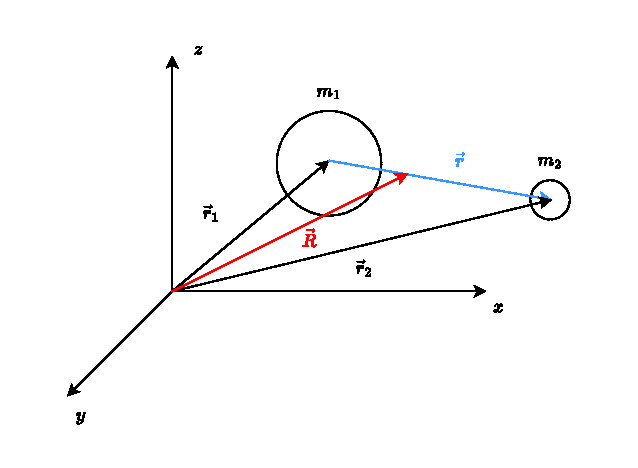
\includegraphics[width=0.8\linewidth]{res/svg/two_body_problem_start.drawio}
  \caption{Two body problem}
\end{figure}
In principle we start from $3n= 6$ degrees of freedom, which means that $\vec{r}_1$ and $\vec{r}_2$ can be used as $q_{\alpha}$, but, in order to use Kőnig's theorem we can define the coordinate of the centre of mass:
\begin{equation}
  \vec{R} = \dfrac{m_1\vec{r}_1 + m_2\vec{r}_2}{m_1 + m_2}
\end{equation}
Since the potential $V(r)$ only depends on the distance between the objects we can define the vector that goes from $m_1$ to $m_2$ as:
\begin{equation}
  \vec{r} = \vec{r}_2 - \vec{r}_1
\end{equation}
From this we can obtain the transformation equations. First we find $\vec{r_1}$:
\begin{equation}
  \begin{split}
    \vec{R} &= \dfrac{m_1\vec{r}_1 + m_2\vec{r}_2}{m_1 + m_2} \\[8pt]
    \vec{R} - \vec{r}_1 &= \dfrac{m_1\vec{r}_1 + m_2\vec{r}_2}{m_1 + m_2} - \vec{r}_1 \\[8pt]
    \vec{R} - \vec{r}_1 &= \dfrac{\cancel{m_1\vec{r}_1} - \cancel{m_1\vec{r}_1} + m_2\vec{r}_2 - m_2\vec{r}_1}{m_1 + m_2} \\[8pt]
    \vec{R} - \vec{r}_1 &= \dfrac{m_2(\overbrace{\vec{r}_2 - \vec{r}_1}^{\vec{r}})}{m_1 + m_2} \\[8pt]
    \vec{r}_1 &= \vec{R} - \dfrac{m_2}{m_1 + m_2}\vec{r}
  \end{split}
\end{equation}
Same goes for $\vec{r}_2$
\begin{equation}
  \begin{split}
    \vec{R} &= \dfrac{m_1\vec{r}_1 + m_2\vec{r}_2}{m_1 + m_2} \\[8pt]
    \vec{R} - \vec{r}_2 &= \dfrac{m_1\vec{r}_1 + m_2\vec{r}_2}{m_1 + m_2} - \vec{r}_2 \\[8pt]
    \vec{R} - \vec{r}_2 &= \dfrac{\cancel{m_2\vec{r}_2} - \cancel{m_2\vec{r}_2} + m_1\vec{r}_1 - m_1\vec{r}_2}{m_1 + m_2} \\[8pt]
    \vec{R} - \vec{r}_2 &= -\dfrac{m_1(\overbrace{\vec{r}_2 - \vec{r}_1}^{\vec{r}})}{m_1 + m_2} \\[8pt]
    \vec{r}_2 &= \vec{R} + \dfrac{m_1}{m_1 + m_2}\vec{r}
  \end{split}
\end{equation}
We can further simplify those equations by introducing the \textbf{reduced mass} $\mu$:
\begin{equation}
  \mu \defineeq \dfrac{m_1 m_2}{m_2 + m_1}
\end{equation}
And so the transformation equations can be written as:
\begin{equation}
  \begin{cases}
    \vec{r}_1 = \vec{R} - \dfrac{\mu}{m_1}\vec{r} \\[8pt]
    \vec{r}_2 = \vec{R} + \dfrac{\mu}{m_2}\vec{r}
  \end{cases}
\end{equation}
The transformation equations do not depend on time, so the Hamiltonian is the energy and it is conserved. The kinetic energy $T$ is a quadratic function of the velocity since the system does not have any external force and so we can finally apply Kőnig's theorem:
\begin{equation}
  T = T_{CM} + T'
\end{equation}
$T'$ is the kinetic energy in the reference frame of the centre of mass. If we use the transformation equations we can recover those terms:
\begin{equation}
  \begin{split}
    T &= \dfrac{1}{2}m_1\dvec{r}_1^2 + \dfrac{1}{2}m_1\dvec{r}_1^2 = \\[8pt]
    &= \dfrac{1}{2}m_1\brackets{\dvec{R} - \dfrac{\mu}{m_1}\dvec{r}}^2 + \dfrac{1}{2}m_2\brackets{\dvec{R} + \dfrac{\mu}{m_2}\dvec{r}}^2 = \\[8pt]
    &= \dfrac{1}{2}m_1\brackets{\dvec{R}^2 - 2\dfrac{\mu}{m_1}\dvec{r}\dvec{R} + \dfrac{\mu^2}{m_1^2}\dvec{r}^2} + \dfrac{1}{2}m_2\brackets{\dvec{R}^2 + 2\dfrac{\mu}{m_2}\dvec{r}\dvec{R} + \dfrac{\mu^2}{m_2^2}\dvec{r}^2} = \\[8pt]
    &= \dfrac{1}{2}m_1\dvec{R}^2 - \cancel{\mu\dvec{r}\dvec{R}} + \dfrac{\mu^2}{2m_1}\dvec{r}^2 + \dfrac{1}{2}m_2\dvec{R}^2 + \cancel{\mu \dvec{r}\dvec{R}} + \dfrac{\mu^2}{2m_2}\dvec{r}^2 = \\[8pt]
    &= \dfrac{1}{2}\brackets{m_1 + m_2}\dvec{R}^2 + \dfrac{1}{2}\brackets{\mu^2\underbrace{\dfrac{m_1 + m_2}{m_1m_2}}_{\mu}}\dvec{r}^2 = \\[8pt]
    &= \dfrac{1}{2}M\dvec{R}^2 + \dfrac{1}{2}\mu\dvec{r}^2
  \end{split}
\end{equation}
Clearly we have:
\begin{equation}
  \begin{split}
    &T_{CM} = \dfrac{1}{2}M\dvec{R}^2 \\[8pt]
    &T' = \dfrac{1}{2}\mu\dvec{r}^2
  \end{split}
\end{equation}
We can thus construct the Lagrangian of the system for a general potential $V(r)$:
\begin{equation}
  \lagr = T - V = \dfrac{1}{2}M\dvec{R}^2 + \dfrac{1}{2}\mu\dvec{r}^2 - V(r)
\end{equation}
The components of the centre of mass $X, Y, Z$ do not appear in the Lagrangian and so we immediately find that their conjugate momenta $p_X, p_Y, p_Z$ are conserved, thus the total momentum of the centre of mass $\vec{P}$ is conserved, but we know that:
\begin{equation}
  \vec{P} = M\dvec{R}
\end{equation}
And since the mass is constant also $\dvec{R}$ will be a conserved quantity and the centre of mass moves with constant velocity, thus we can ignore this term in the Lagrangian. We define the new Lagrangian as:
\begin{equation}
  \lagr ' = \dfrac{1}{2}\mu\dvec{r}^2 - V(r)
\end{equation}
Since the potential $V(r)$ only depends on the distance of the masses it is spherically simmetric, which implies that the Lagrangian is spherically simmetric and so $L_x, L_y, L_z$ are conserved quantities, but also $\vec{L}$ is conserved. $\vec{L}$ is the angular momentum about the centre of mass:
\begin{equation}
  \vec{L} = \vec{r}\cross \mu\dvec{r}
\end{equation}
And so the orbit must take place in the plane perpendicular to $\vec{L}$.
\begin{figure}[H]
  \centering
  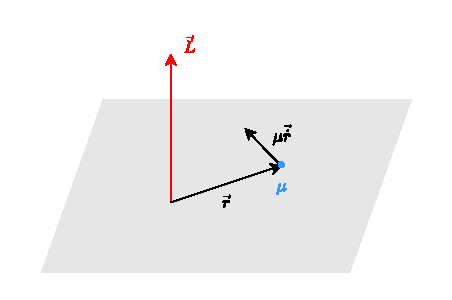
\includegraphics[width=0.6\linewidth]{res/svg/two_body_problem_angular.drawio}
\end{figure}
\begin{figure}[H]
  \centering
  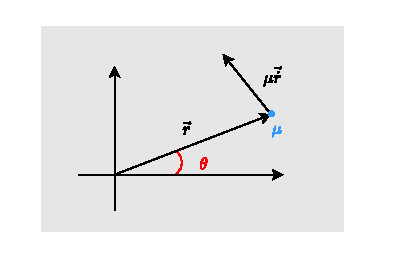
\includegraphics[width=0.6\linewidth]{res/svg/two_body_problem_angular_plane.drawio}
  \caption{Plane orbit}
\end{figure}
Using this fact we can switch to radial coordinates and rewrite the Lagrangian as:
\begin{equation}
  \lagr' = \dfrac{1}{2}\mu\brackets{\dot{r}^2 + r^2\dot{\theta}^2} - V(r)
\end{equation}
Here $\theta$ does not appear and so it is a cyclic coordinate, which means that $p_{\theta}$ is conserved:
\begin{equation}
  p_{\theta} = \pdv{\lagr'}{\dot{\theta}} = \mu r^2 \dot{\theta}
\end{equation}
But this is also the $z$ component of the angular momentum:
\begin{equation}
  \begin{split}
    L_z &= \brackets{\vec{r}\cross \mu\dvec{r}} \cdot \hat{u}_z = \\[8pt]
    &= \sqbr{r\hat{u}_r \cross \mu\brackets{\dot{r}\hat{u}_r + r\dot{\theta}\hat{u}_{\theta}}} \cdot \hat{u}_z = \\[8pt]
    &= \bbrackets{\mu r\dot{r} \cancel{\hat{u}_r \cross \hat{u}_r} + \mu r^2\dot{\theta}\underbrace{\hat{u}_r \cross \hat{u}_{\theta}}_{\hat{u}_z}} \cdot \hat{u}_z = \\[8pt]
    &= \mu r^2\dot{\theta} \hat{u}_z \cdot \hat{u}_z = \mu r^2\dot{\theta}
  \end{split}
\end{equation}
And thus we have:
\begin{equation}
  \dot{\theta} = \dfrac{L_z}{\mu \dot{r}^2}
\end{equation}
Now we can apply \eleref\;to $\lagr'$ for $q_{\alpha} = r$ and see what we get:
\begin{equation}
  \begin{split}
    &\dv{}{t}\pdv{}{\dot{r}}\brackets{\dfrac{1}{2}\mu\brackets{\dot{r}^2 + r^2\dot{\theta}^2} - V(r)} - \pdv{}{r}\brackets{\dfrac{1}{2}\mu\brackets{\dot{r}^2 + r^2\dot{\theta}^2} - V(r)} = \\[8pt]
    &= \mu\dv{\dot{r}}{t} - \mu r\dot{\theta}^2 + \pdv{V}{r}  = \\[8pt]
    &= \mu \ddot{r} - \mu r\dot{\theta}^2 + \pdv{V}{r}
  \end{split}
\end{equation}
Now we can substitute what we got for $\dot{\theta}$:
\begin{equation} \label{ele_twobody}
  \boxed{\mu \ddot{r} - \dfrac{L_z^2}{\mu \dot{r}^3} + \pdv{V}{r} = 0}
\end{equation}
Remember that we want to write this problem as a one dimensional problem, so we need to find a potential of the type:
\begin{equation}
  m\dot{q} = -\pdv{V}{q}
\end{equation}
We can rewrite the term with $L_z$ as:
\begin{equation}
  - \dfrac{L_z^2}{\mu \dot{r}^3} = \pdv{}{r}\brackets{\dfrac{L_z^2}{2\mu \dot{r}^2}}
\end{equation}
From \eqref{ele_twobody} we get:
\begin{equation}
  \mu \ddot{r} = -\pdv{}{r}\brackets{V - \dfrac{L_z^2}{2\mu \dot{r}^2}}
\end{equation}
By multiplying both sides by $\dot{r}$ we get the total time derivative of $\dfrac{1}{2}\mu \dot{r}^2$ on the left side and the total time derivative of the quantity in brackets of the right side since it only depends on $r$. We will that quantity \textbf{effective potential} $V_{\text{eff}}$, since it is not a real potential, but it will serve the purpose of the one dimensional potential that we want to find. We can write:
\begin{equation}
    \begin{split}
        &\mu \ddot{r}\dot{r} = -\pdv{V_{\text{eff}}(r)}{r}\dot{r} \\[8pt]
        &\dv{}{t}\brackets{\dfrac{1}{2}\mu \dot{r}^2} = -\dv{V_{\text{eff}}}{t} \\[8pt]
        &\dv{}{t}\brackets{\dfrac{1}{2}\mu \dot{r}^2 + V_{\text{eff}}} = 0
    \end{split}
\end{equation}
From the last equation we know that the quantity in brackets is conserved. We still have not used the conservation of energy. The total energy is:
\begin{equation}
    E = \dfrac{1}{2}\mu \dot{r}^2 + V - \dfrac{L_z^2}{2\mu \dot{r}^2}
\end{equation}
And so we can find $r$ by integrating. We have:
\begin{equation}
    \begin{split}
        \dfrac{1}{2}\mu \dot{r}^2 = E - V + \dfrac{L_z^2}{2\mu \dot{r}^2} \\[8pt]
        \dot{r}^2 = \dfrac{2}{\mu}\brackets{E - V + \dfrac{L_z^2}{2\mu \dot{r}^2}} \\[8pt]
        \dv{r}{t} = \pm\sqrt{\dfrac{2}{\mu}\brackets{E - V + \dfrac{L_z^2}{2\mu \dot{r}^2}}} \\[8pt]
        \int_{r(0)}^{r(t)}\pm\sqrt{\dfrac{\mu}{2\brackets{E - V + \frac{L_z^2}{2\mu \dot{r}^2}}}}\diff{r} = \int_{0}^{t}\diff{t}
    \end{split}
\end{equation}
If $V(r)$ is known we can solve this integral and get $t$ as a function of $r(t)$:
\begin{equation}
  t = f(r(t)) \xrightarrow{\text{invert}} r = r(t)
\end{equation}
We also need to find $\theta(t)$ to get the transverse velocity:
\begin{equation}
  \begin{split}
    &\dv{\theta}{t} = \dfrac{L_z^2}{\mu \dot{r}^2} \\[8pt]
    &\int_{\theta(0)}^{\theta}\diff{\theta} = \int_{0}^{t}\dfrac{L_z^2}{\mu \dot{r}^2}\diff{t} \\[8pt]
    &\theta(t) = \theta(0) + \int_{0}^{t}\dfrac{L_z^2}{\mu \dot{r}^2}\diff{t}
  \end{split}
\end{equation}
Now we can use the fact that:
\begin{equation}
  \diff{t} = \pm\sqrt{\dfrac{\mu}{2\brackets{E - V + \frac{L_z^2}{2\mu \dot{r}^2}}}}\diff{r}
\end{equation}
We can limit ourselves to the case of $+$ since $L_z$ has a constant sign and so we can ``absorb'' the $\pm$ with the choice of $L_z$. We arrive to the expression:
\begin{equation}
  \theta(t) = \theta(0) + \int_{a}^{b}\dfrac{L_z^2}{\mu \dot{r}^2}\sqrt{\dfrac{\mu}{2\brackets{E - V + \frac{L_z^2}{2\mu \dot{r}^2}}}}\diff{r}
\end{equation}
The limits of the integral change since we made a change of variable. They are unkown for the moment since we have no form of $V$. Now we need the intial conditions:
\begin{itemize}
  \item $r(0) = r_0$
  \item $\dot{r}(0) = \dot{r}_0$
  \item $\theta(0) = \theta_0$
  \item $\dot{\theta}(0) = \dot{\theta}_0$
\end{itemize}
We can fix $\dot{r}_0$ and $\dot{\theta}_0$ with $L_z$ and $E$ since they are conserved:
\begin{equation}
  L_z = \mu r_0^2 \dot{\theta}_0^2 \implies \dot{\theta}_0^2 = \dfrac{L_z}{\mu r_0^2}
\end{equation}
\begin{equation}
  E = \dfrac{1}{2}\mu\dot{r}_0^2 + V_{\text{eff}}(r_0) \implies \dot{r}_0 = \pm\sqrt{\dfrac{2}{\mu}\brackets{E - V_{\text{eff}}(r_0)}}
\end{equation}
In general we have:
\begin{equation}
    \dot{r}(t) = \pm\sqrt{\dfrac{2}{\mu}\brackets{E - V_{\text{eff}}(t)}}
\end{equation}
And so $r(t)$ cannot be a monotonic function, but there must exist a point of inversion. This point is found when the time derivative is zero:
\begin{equation}
    \pm\sqrt{\dfrac{2}{\mu}\brackets{E - V_{\text{eff}}(t)}} = 0 \implies E = V_{\text{eff}}
\end{equation}
This means that when $V_{\text{eff}}$ is equal to the energy we have a point of inversion. Since $V_{\text{eff}} = V + \dfrac{L_z}{2\mu r^2}$ depending on $V$ and $E$ we can have either $1$ or $2$ points of inversion.
\begin{itemize}
    \item If only $1$ point is present we just have a one time motion. The object comes from infinity, orbits the other one for a certain period and then goes away.
    \item If two points of inversion are present the motion of $\mu$ is limited in a certain angular region with a maximum and a minimum
\end{itemize}
Notice that the orbits are not necessarily closed.
\subsection{The Kepler problem}
As an example we will discuss the Kepler problem, which describes how orbits work in the case of a potential of the type:
\begin{equation}
    V(r) = -\dfrac{\alpha}{r}
\end{equation}
This could be for example the gravitational potential or the Coulomb potential. Given this form of $V$ we know that:
\begin{equation}
    V_{\text{eff}} = \dfrac{L_z^2}{2 \mu r^2} - \dfrac{\alpha}{r}
\end{equation}
Qualitatively speaking we know the asymptotic behavior of the effective potential:
\begin{itemize}
    \item At $r \rightarrow 0$ the term with $\dfrac{1}{r^2}$ dominates so $V_{\text{eff}} \rightarrow +\infty$ for $r \rightarrow 0$
    \item For $r \rightarrow +\infty$ the term with $-\dfrac{1}{r}$ dominates so $V_{\text{eff}} \rightarrow -$ for $r \rightarrow 0$ with negative values
    \item There must be a point where $V_{\text{eff}}$ stops decreasing and starts increasing, this is a point of minimum for the effective potential
\end{itemize}
\begin{figure}[H]
  \centering
  \includesvg[width=0.8\linewidth]{res/svg/effectivepotential_sum}
\end{figure}
Let's find the minimum:
\begin{equation}
  \pdv{}{r}\brackets{\dfrac{L_z^2}{2 \mu r^2} - \dfrac{\alpha}{r}} =  \dfrac{\alpha}{r^2} -\dfrac{L_z^2}{\mu r^3}
\end{equation}
Setting this to zero gives:
\begin{equation}
  \dfrac{\alpha}{\cancel{r^2}} =\dfrac{L_z^2}{\mu r^{\cancel{3}}} \implies r = \dfrac{L_z^2}{\mu \alpha}
\end{equation}
If we compare $V_{\text{eff}}$ to a constant value of energy we find that the point of intersection is where $E = V_{\text{eff}}$ and so where $\dot{r} = 0$, which is the inversion point of the orbit. We can distinguish 4 cases.\\
\textbf{Case 1.} In the first case we have $E > 0$.
\begin{figure}[H]
  \centering
  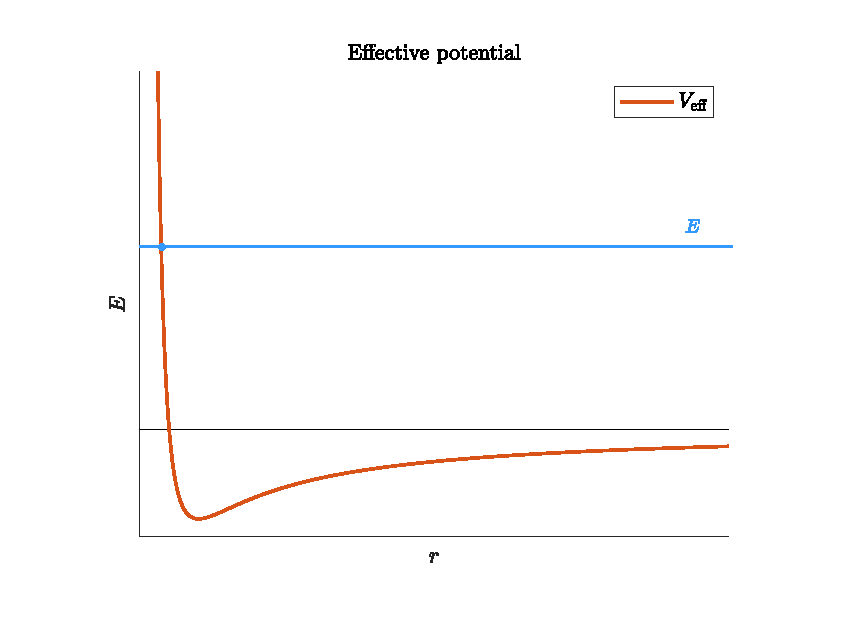
\includegraphics[width=0.6\linewidth]{res/svg/hyperbolic_orbit.drawio}
\end{figure}
There is only one point of inversion and the orbit is hyperbolic.
\begin{figure}[H]
  \centering
  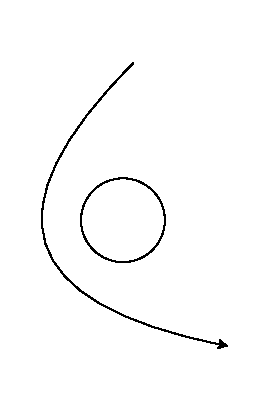
\includegraphics[width=0.2\linewidth]{res/svg/hyperbolic_orbit_drawing.drawio}
\end{figure}
\textbf{Case 2.} In the second case we have $E = 0$.
\begin{figure}[H]
  \centering
  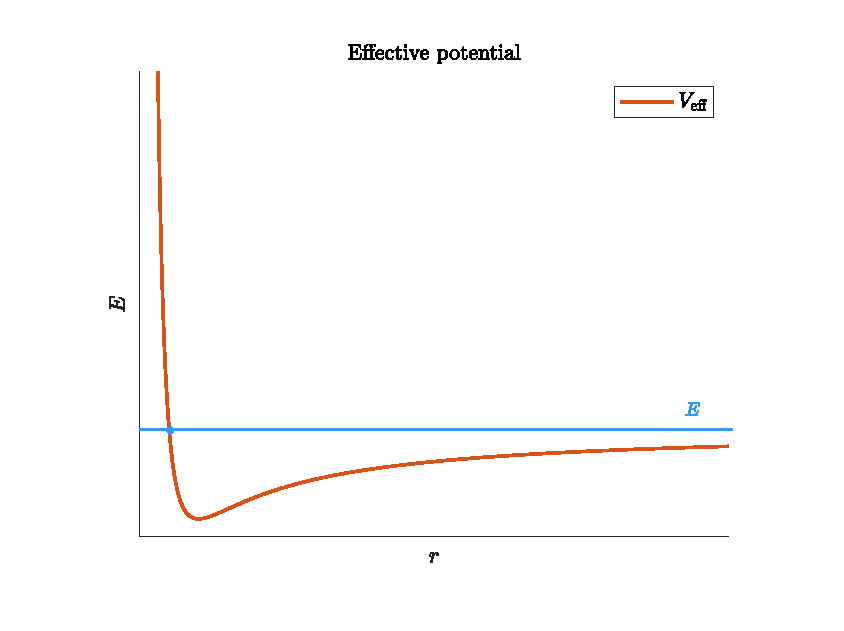
\includegraphics[width=0.6\linewidth]{res/svg/parabolic_orbit.drawio}
\end{figure}
Here we have one point of inversion and we also have that $E=V_{\text{eff}}$ at infinity. This creates a parabolic orbit.
\begin{figure}[H]
  \centering
  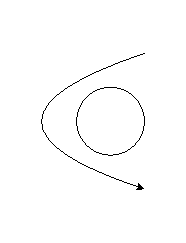
\includegraphics[width=0.2\linewidth]{res/svg/parabolic_orbit_drawing.drawio}
\end{figure}
\textbf{Case 3.} In the third case $E<0$ but it is greater than the minimum of $V_{\text{eff}}$.
\begin{figure}[H]
  \centering
  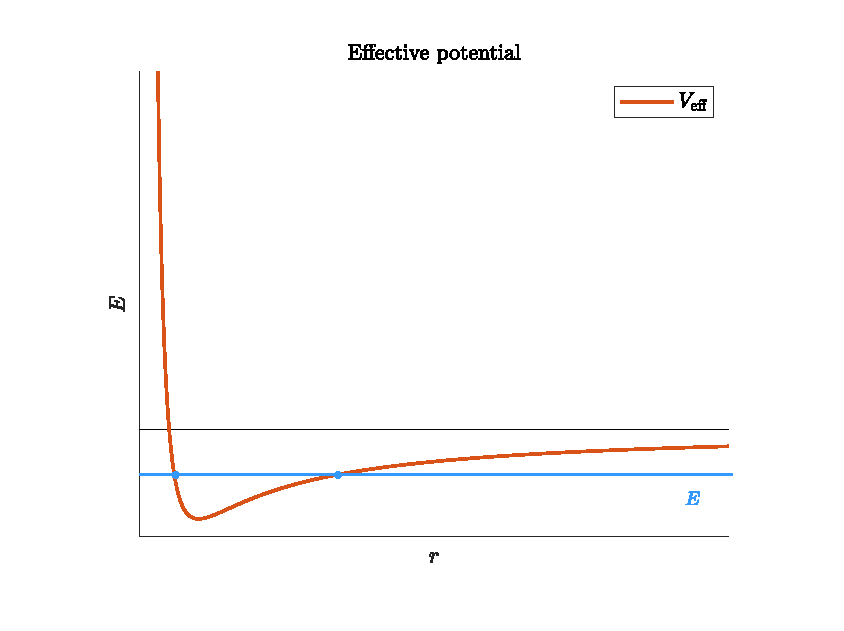
\includegraphics[width=0.6\linewidth]{res/svg/elliptic_orbit.drawio}
\end{figure}
We have two distinct inversion points $r_0$ and $r_1$ which create an elliptical orbit.
\begin{figure}[H]
  \centering
  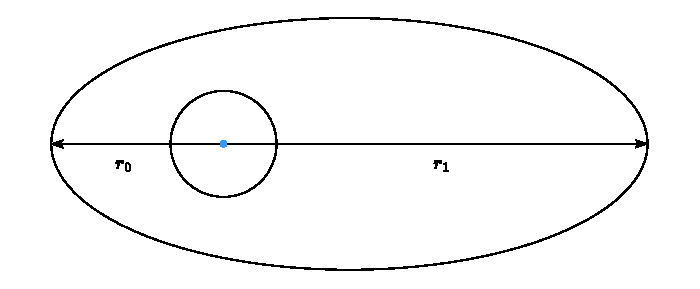
\includegraphics[width=0.6\linewidth]{res/svg/elliptic_orbit._drawing.drawio}
\end{figure}
\textbf{Case 4.} In the fourth case $E<0$ and it is equal to the minimum of $V_{\text{eff}}$.
\begin{figure}[H]
  \centering
  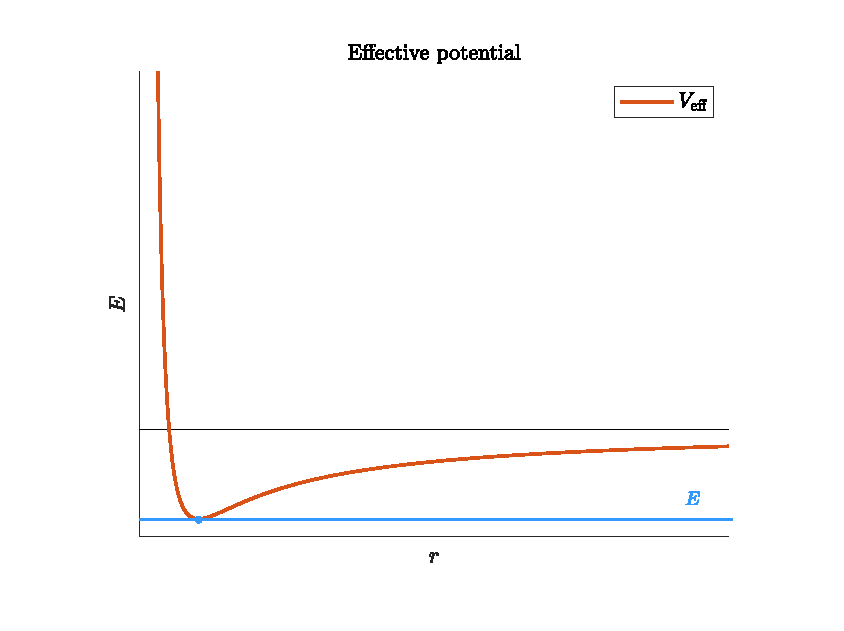
\includegraphics[width=0.6\linewidth]{res/svg/circular_orbit.drawio}
\end{figure}
We have two coincident inversion points which create a circular orbit.
\begin{figure}[H]
  \centering
  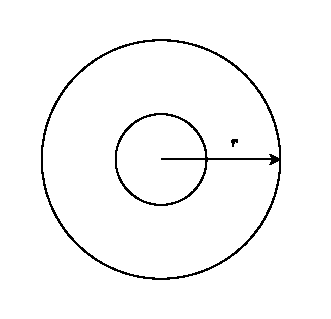
\includegraphics[width=0.4\linewidth]{res/svg/circular_orbit_drawing.drawio}
\end{figure}

\chapter{Canonical transformations}
\section{Point transformations}
Let's now focus on the possible transformations of coordinates.\\
In Lagrangian formalism a generic transformation is:
\begin{equation}
    \{q_{\alpha}\} \longrightarrow \{Q_{\alpha}\}\quad \text{s.t.}\quad Q_{\alpha} = Q_{\alpha}\brackets{q_1,q_2,\dots,q_n,t}
\end{equation}
This is a \textbf{point transformation} in configuration space. We move from $n$ spatial coordinates to $n$ spatial coordinates.\\
In Hamiltonian formalism a generic transformation is:
\begin{equation}
    \begin{Bmatrix}
        q_{\alpha}\\[8pt]
        p_{\alpha}
    \end{Bmatrix} \longrightarrow
    \begin{Bmatrix}
        Q_{\alpha}\\[8pt]
        P_{\alpha}
    \end{Bmatrix}\quad \text{s.t} \quad
    \begin{cases}
        Q_{\alpha} = Q_{\alpha}\brackets{q_1,q_2,\dots,q_n,p_1,p_2,\dots,p_n,t}\\
        P_{\alpha} = P_{\alpha}\brackets{q_1,q_2,\dots,q_n,p_1,p_2,\dots,p_n,t}
    \end{cases}
\end{equation}
This is also a point transformation, but since we are in the phase space the new coordinates can be a mix of both $q_{\alpha}$ and $p_{\alpha}$. Now we can try to figure out if the relations found for $q_{\alpha}$ and $p_{\alpha}$ related to the Poisson brackets are also true for $Q_{\alpha}$ and $P_{\alpha}$.
We want:
\begin{equation}
    \begin{split}
        \pb{q_{\alpha}}{q_{\beta}} &= 0\\
        \pb{p_{\alpha}}{p_{\beta}} &= 0\\
        \pb{q_{\alpha}}{p_{\beta}} &= \delta_{\alpha \beta}
    \end{split} \implies
    \begin{split}
        \pb{Q_{\alpha}}{Q_{\beta}} &= 0\\
        \pb{P_{\alpha}}{P_{\beta}} &= 0\\
        \pb{Q_{\alpha}}{P_{\beta}} &= \delta_{\alpha \beta}
    \end{split}
\end{equation}
For example we want $\pb{Q_{\alpha}}{Q_{\beta}} = 0$. If we explicit the Poisson brackets we have:
\begin{equation}
    \pb{Q_{\alpha}}{Q_{\beta}} = \bigsum_{\gamma} \left(\pdv{Q_{\alpha}}{q_{\gamma}} \pdv{Q_{\beta}}{p_{\gamma}} - \pdv{Q_{\alpha}}{p_{\gamma}} \pdv{Q_{\beta}}{q_{\gamma}} \right)
\end{equation}
This is not always zero, therefor we will look for transformations such that:
\begin{equation}
    \begin{cases}
        \dot{Q}_{\alpha} = \pdv{\tilde{\hamfun}}{P_{\alpha}} \\[8pt]
        \dot{P}_{\alpha} = -\pdv{\tilde{\hamfun}}{Q_{\alpha}}
    \end{cases}
\end{equation}
Transformations that preserve those properties are called \textbf{canonical transformations}. The new Hamiltonian associated to those transformations is sometimes called \textit{k-Hamiltonian}.\\
In which condition this is true?\\
Recall that the \hamiltonref\;come from the \hpquotemath :
\begin{equation}
    \delta \action = \delta \int_{t_1}^{t_2}\lagr \dd{t} = \int_{t_1}^{t_2} \brackets{\bigsum_{\alpha}\dot{q}_{\alpha}p_{\alpha} - \hamfun} \dd{t} =0
\end{equation}
We want the same for the new Hamiltonian:
\begin{equation}
    \delta \tilde{\action} = \delta \int_{t_1}^{t_2}\tilde{\lagr} \dd{t} \int_{t_1}^{t_2} \brackets{\bigsum_{\alpha}\dot{Q}_{\alpha}P_{\alpha} - \tilde{\hamfun}} \dd{t} \overset{!}{=} 0
\end{equation}
\section{Generating functions}
We also know that the new Lagrangian and the old Lagrangian must describe the same system and they have this relation:
\begin{equation}
    \lagr = \tilde{\lagr}+\dv{F}{t}
\end{equation}
So there must exist a function $F$ such that this is true for a transformation to be canonical. These functions are called \textbf{generating functions}.
In principle a generic $F$ can depend on both the old and the new coordinates:
\begin{equation}
    F = F(\vec{q},\vec{p},\vec{Q},\vec{P},t)
\end{equation}
But if all the coordinates were independent we would have $4n$ variables plus time. The maximum number of variables is $2n$ hence there must be at least $2n$ dependent variables.\\
If we know the expression for both the generating function and the transformation equations we are done. This of course is not the interesting case. We can reconstruct the transformation equations just from the expression of $F$. We can distinguish 4 categories of generating functions:
\begin{enumerate}
    \item $F_1 = F_1(\vec{q},\vec{Q},t)$ (\nth{1} type functions)
    \item $F_2 = F_2(\vec{q},\vec{P},t)$ (\nth{2}  type functions)
    \item $F_3 = F_3(\vec{p},\vec{Q},t)$ (\nth{3}  type functions)
    \item $F_4 = F_4(\vec{p},\vec{P},t)$ (\nth{4}  type functions)
\end{enumerate}
From the relation between the Lagrangians we have:
\begin{equation}
    \begin{split}
        \lagr &= \tilde{\lagr}+\dv{F}{t}\\
        \bigsum_{\alpha}p_{\alpha}\dd{q_{\alpha}} - \hamfun\dd{t} &= \bigsum_{\alpha}P_{\alpha}\dd{Q_{\alpha}} - \tilde{\hamfun}\dd{t} + \dd{F}\\
        &\Downarrow \\
        \dd{F} = \bigsum_{\alpha}p_{\alpha}\dd{q_{\alpha}} &- \bigsum_{\alpha}P_{\alpha}\dd{Q_{\alpha}} + \brackets{\tilde{\hamfun}- \hamfun}\dd{t}\\
        &\Downarrow \\
        F &= F(\vec{q},\vec{Q})
    \end{split}
\end{equation}
This means that the generating function in the relation with the Lagrangians is a first type function $F = F_1$. In this case the differential of $F_1$ is:
\begin{equation}
    \dd{F_1} = \bigsum_{\alpha} \pdv{F_1}{q_{\alpha}} \dd{q_{\alpha}} + \bigsum_{\alpha} \pdv{F_1}{Q_{\alpha}} \dd{Q_{\alpha}} + \pdv{F_1}{t} \dd{t}
\end{equation}
And so we get:
\begin{equation} \label{F1_Canonical}
    \begin{cases}
        \pdv{F_1}{q_{\alpha}} = p_{\alpha}\\[8pt]
        \pdv{F_1}{Q_{\alpha}} = -P_{\alpha}\\[8pt]
        \pdv{F_1}{t} = \brackets{\tilde{\hamfun}- \hamfun}
    \end{cases}
\end{equation}
Hence:
\begin{equation}
    \begin{cases}
        p = p(\vec{q},\vec{Q},t)\\
        P = P(\vec{q},\vec{Q},t)
    \end{cases}
\end{equation}
By inverting the first equation we can get:
\begin{equation}
    Q = Q(\vec{q},\vec{p},t)\\
\end{equation}
Substituting this into the second equation we finally get the transformation equations:
\begin{equation}
    \begin{cases}
        Q = Q(\vec{q},\vec{p},t)\\
        P = P(\vec{q},\vec{p},t)
    \end{cases}
\end{equation}
Also from the third equation in \eqref{F1_Canonical} we have:
\begin{equation}
    \tilde{\hamfun} = \hamfun + \pdv{F_1}{t}
\end{equation}
And so if $F_1$ does not depend on time explicitly:
\begin{equation}
    \tilde{\hamfun} = \hamfun
\end{equation}
This means that the Hamiltonians are equal, but we need to keep in mind that $\tilde{\hamfun}$ depends on the new coordinates so if we have a generic $\hamfun$ substituting $Q$ and $P$ instead of $q$ and $p$ \underline{does not} give $\tilde{\hamfun}$. For example:
\begin{equation}
    \hamfun = \dfrac{p^2}{2m} + \dfrac{\alpha}{q} \notimplies \tilde{\hamfun} = \dfrac{P^2}{2m} + \dfrac{\alpha}{Q}
\end{equation}
Instead we need to substitute the expression of the old coordinates in terms of the new one (or viceversa if we have $\tilde{\hamfun}$).\\
Now let $F$ be a generating function of the first type but with:
\begin{equation}
    \begin{cases}
        Q = q\\
        P = P(\vec{q},\vec{p},t)
    \end{cases}
\end{equation}
Then $q$ and $Q$ are not independent, therefor we should have only $n$ independent variables in $F$, but this is not what we want. In order to write $F$ in terms of only independent coordinates we must find a way to express $F$ as a second type function:
\begin{equation}
    F_1(\vec{q},\vec{Q},t) \longrightarrow F_2(\vec{q},\vec{P},t)
\end{equation}
This is just an application of the Legendre transformations:
\begin{equation}
    \begin{split}
        \dd{F_1} &= \bigsum_{\alpha}p_{\alpha}\dd{q_{\alpha}} - \bigsum_{\alpha}P_{\alpha}\dd{Q_{\alpha}} + \brackets{\tilde{\hamfun}- \hamfun}\dd{t}\\
        \dd{\brackets{F_1 + \bigsum_{\alpha}P_{\alpha}Q_{\alpha}}} &= \bigsum_{\alpha}p_{\alpha}\dd{q_{\alpha}}  + \bigsum_{\alpha}Q_{\alpha}\dd{P_{\alpha}} + \brackets{\tilde{\hamfun}- \hamfun}\dd{t}
    \end{split}
\end{equation}
And so:
\begin{equation}
    F_2 = F_1 + \bigsum_{\alpha}P_{\alpha}Q_{\alpha}
\end{equation}
From this, we obtain the relations:
\begin{equation}
    \begin{cases}
        \pdv{F_2}{q_{\alpha}} = p_{\alpha}\\[8pt]
        \pdv{F_2}{P_{\alpha}} = Q_{\alpha}\\[8pt]
        \pdv{F_2}{t} = \pdv{F_1}{t}
    \end{cases}
\end{equation}
As for the first type this means that:
\begin{equation}
    \begin{cases}
        p = p(\vec{q},\vec{P},t)\\
        Q = P(\vec{q},\vec{P},t)
    \end{cases}
\end{equation}
By inverting the first equation we can get:
\begin{equation}
    P = P(\vec{q},\vec{p},t)\\
\end{equation}
Substituting this into the second equation we get the transformation equations:
\begin{equation}
    \begin{cases}
        Q = Q(\vec{q},\vec{p},t)\\
        P = P(\vec{q},\vec{p},t)
    \end{cases}
\end{equation}
Similarly we can find a way to express $F_1$ as a third type function $F_3$. This is again an application of the Legendre transformations:
\begin{equation}
    \begin{split}
        \dd{F_1} = \bigsum_{\alpha}p_{\alpha}\dd{q_{\alpha}} - \bigsum_{\alpha}P_{\alpha}\dd{Q_{\alpha}} + \brackets{\tilde{\hamfun}- \hamfun}\dd{t}\\
    \dd{\brackets{F_1 - \bigsum_{\alpha}q_{\alpha}p_{\alpha}}} = -\bigsum_{\alpha}q_{\alpha}\dd{p_{\alpha}} - \bigsum_{\alpha}P_{\alpha}\dd{Q_{\alpha}} + \brackets{\tilde{\hamfun}- \hamfun}\dd{t}
    \end{split}
\end{equation}
And so:
\begin{equation}
    F_3 = F_1 - \bigsum_{\alpha}q_{\alpha}p_{\alpha}
\end{equation}
From this, we obtain the relations:
\begin{equation}
    \begin{cases}
        \pdv{F_3}{p_{\alpha}} = -q_{\alpha}\\[8pt]
        \pdv{F_3}{Q_{\alpha}} = -P_{\alpha}\\[8pt]
        \pdv{F_3}{t} = \pdv{F_1}{t}
    \end{cases}
\end{equation}
As for the first type, this means that:
\begin{equation}
    \begin{cases}
        q = q(\vec{p},\vec{Q},t)\\
        P = P(\vec{p},\vec{Q},t)
    \end{cases}
\end{equation}
By inverting the first equation, we can get:
\begin{equation}
    Q = Q(\vec{q},\vec{p},t)
\end{equation}
Substituting this into the second equation, we get the transformation equations:
\begin{equation}
    \begin{cases}
        Q = Q(\vec{q},\vec{p},t)\\
        P = P(\vec{q},\vec{p},t)
    \end{cases}
\end{equation}
Finally we can find a way to express $F_1$ as a fourth type function $F_4$. This is a double application of the Legendre transformations (we can think to pass through second type first or third type first and then go to fourth type):
\begin{equation}
    \begin{split}
        \dd{F_1} &= \bigsum_{\alpha}p_{\alpha}\dd{q_{\alpha}} - \bigsum_{\alpha}P_{\alpha}\dd{Q_{\alpha}} + \brackets{\tilde{\hamfun}- \hamfun}\dd{t}\\
        \dd{\brackets{F_1 + \bigsum_{\alpha}P_{\alpha}Q_{\alpha} - \bigsum_{\alpha}q_{\alpha}p_{\alpha}}} &= -\bigsum_{\alpha}q_{\alpha}\dd{p_{\alpha}} + \bigsum_{\alpha}Q_{\alpha}\dd{P_{\alpha}} + \brackets{\tilde{\hamfun}- \hamfun}\dd{t}
    \end{split}
\end{equation}
And so:
\begin{equation}
    F_4 = F_1 + \bigsum_{\alpha}P_{\alpha}Q_{\alpha} - \bigsum_{\alpha}q_{\alpha}p_{\alpha}
\end{equation}
From this, we obtain the relations:
\begin{equation}
    \begin{cases}
        \pdv{F_4}{p_{\alpha}} = -q_{\alpha}\\[8pt]
        \pdv{F_4}{P_{\alpha}} = Q_{\alpha}\\[8pt]
        \pdv{F_4}{t} = \pdv{F_1}{t}
    \end{cases}
\end{equation}
As for the first type, this means that:
\begin{equation}
    \begin{cases}
        q = q(\vec{p},\vec{P},t)\\
        Q = Q(\vec{p},\vec{P},t)
    \end{cases}
\end{equation}
By inverting the first equation, we can get:
\begin{equation}
    P = P(\vec{q},\vec{p},t)
\end{equation}
Substituting this into the second equation, we get the transformation equations:
\begin{equation}
    \begin{cases}
        Q = Q(\vec{q},\vec{p},t)\\
        P = P(\vec{q},\vec{p},t)
    \end{cases}
\end{equation}
\section{Poisson brackets and canonical transformations}
As we anticipated before we want to know how the Poisson brackets act on the new coordinates. In particular, we state this theorem:
\begin{theorem}{}
  A transformation is canonical if and only if the canonical Poisson brackets are invariant
\end{theorem}
This means that they are the same in the old and new coordinates. For example:
\begin{equation}
    \pb{Q_{\alpha}}{P_{\beta}}_{QP} = \delta_{\alpha \beta} \implies \pb{Q_{\alpha}}{P_{\beta}}_{qp} = \delta_{\alpha \beta}
\end{equation}
The subscript represents in respect to what coordinates we are calculating the Poisson brackets. This theorem also as an important corollary:
\begin{corollary}{}
    If the canonical Poisson brackets are invariant then all Poisson brackets are invariant
\end{corollary}
Which means that for any functions $f$ and $g$ in the phase space:
\begin{equation}
    \pb{f}{g}_{QP} = \pb{f}{g}_{qp} = \pb{f}{g}
\end{equation}
In the last notation (which is the usual one) we do not specify the coordinates since it makes no difference.\\
Another relation that is true in general is:
\begin{equation}
    \dv{f}{t} = \pb{f}{\hamfun} + \pdv{f}{t}
\end{equation}
If we are dealing with a function that is also a constant of the motion then:
\begin{equation}
    \pb{f}{\hamfun} = - \pdv{f}{t}
\end{equation}
If this function also does not depend on time explicitly:
\begin{equation}
    \pb{f}{\hamfun} = 0
\end{equation}
\section{Examples}
We will now show some examples of the application of the Legendre transformations and in general of the utility of the generating functions.
\subsection{Ex. 1}
Given a generating function of the first type $F_1 = F_1(\vec{q},\vec{Q},t)$ such that:
\begin{equation}
    F_1 = \bigsum_{\alpha} q_{\alpha}Q_{\alpha}
\end{equation}
By applying \hamiltonref\;and Legendre transformations we get:
\begin{equation}
    \begin{cases}
        Q_{\beta} = \pdv{F_1}{q_{\beta}} = p_{\beta}\\
        q_{\beta} = \pdv{F_1}{Q_{\beta}} = -P_{\beta}
    \end{cases}
\end{equation}
And so the transformation equations are:
\begin{equation}
    \begin{cases}
        Q_{\alpha} = p_{\alpha}\\
        P_{\alpha} = -q_{\alpha}
    \end{cases}
\end{equation}
So this transformation just swaps the momentum and the position coordinates (taking into account some sign changes).
\subsection{Ex. 2}
Given a generating function of the second type $F_2 = F_2(\vec{q},\vec{P},t)$ such that:
\begin{equation}
    F_2 = \bigsum_{\alpha} q_{\alpha}P_{\alpha}
\end{equation}
By applying \hamiltonref\;and Legendre transformations we get:
\begin{equation}
    \begin{cases}
        P_{\beta} = \pdv{F_2}{q_{\beta}} = p_{\beta}\\
        q_{\beta} = \pdv{F_2}{P_{\beta}} = Q_{\beta}
    \end{cases}
\end{equation}
And so the transformation equations are:
\begin{equation}
    \begin{cases}
        Q_{\alpha} = q_{\alpha}\\
        P_{\alpha} = p_{\alpha}
    \end{cases}
\end{equation}
So this transformation is the \textbf{identity transformation} since the new momenta and positions are equal to the old ones.
\begin{equation}
    \underset{\text{Identity}}{\boxed{F_2 = \bigsum_{\alpha} q_{\alpha}P_{\alpha}}}
\end{equation}
\subsection{Ex. 3}
Given a generating function of the second type $F_2 = F_2(\vec{q},\vec{P},t)$ such that:
\begin{equation}
    F_2 = \bigsum_{\alpha} f_{\alpha}(\vec{q},t) P_{\alpha}
\end{equation}
By applying \hamiltonref\;and Legendre transformations we get:
\begin{equation}
    \begin{split}
        p_{\beta} = \pdv{F_2}{q_{\beta}} = \dots\\
        Q_{\beta} = \pdv{F_2}{P_{\beta}} = f_{\beta}(\vec{q},t)
    \end{split}
\end{equation}
So new positions only depend on old positions, hence this is actually a point transformation in configuration space. This is why any point transformation in configuration space is always canonical.
\subsection{Ex. 4}
Now let the Hamiltonian of a system be:
\begin{equation}
    \hamfun = \dfrac{p^2}{2m} + mgq
\end{equation}
\hamiltonref\;give:
\begin{equation}
    \begin{cases}
        \dot{q} = \pdv{\hamfun}{p} = \dfrac{p}{m}\\[8pt]
        \dot{p} = -\pdv{\hamfun}{q} = -mg
    \end{cases}
\end{equation}
Those are just the Newton's equations for a particle in the gravitational potential. Now let's make a transformation:
\begin{equation}
    F_1 = -\dfrac{Q}{q}
\end{equation}
From this we get:
\begin{equation}
    \begin{cases}
        p = \pdv{F_1}{q} = \dfrac{Q}{q^2}\\[8pt]
        P = -\pdv{F_1}{Q} = \dfrac{1}{q}
    \end{cases}
\end{equation}
From this getting the transformation equations is trivial:
\begin{equation}
    \begin{cases}
        Q = pq^2\\[8pt]
        P = \dfrac{1}{q}
    \end{cases}
\end{equation}
We can invert these relations:
\begin{equation}
    \begin{cases}
        q = \dfrac{1}{P}\\
        p = QP^2
    \end{cases}
\end{equation}
And if we substitute back into the old Hamiltonian we get the new expression:
\begin{equation}
    \tilde{\hamfun} = \dfrac{P^4 Q^2}{2m} + \dfrac{mg}{P}
\end{equation}
This again shows that to get the new Hamiltonian we cannot just substitute $Q$ instead of $q$ and $P$ instead of $p$.\\
Also for the new Lagrangian we have:
\begin{equation}
    \begin{split}
        \lagr &= \tilde{\lagr} + \dv{F_1}{t} =\\
        &= \tilde{\lagr} + \dv{}{t}\brackets{-QP} =\\
        &=\tilde{\lagr} - \dot{Q}P - Q\dot{P}
    \end{split}
\end{equation}
Which gives:
\begin{equation}
    \tilde{\lagr} = \lagr + \dot{Q}P + Q\dot{P}
\end{equation}
We want to check that this is a canonical transformation. We can do this by calculating the canonical Poisson brackets in the new and old coordinates. For the new ones:
\begin{equation}
    \begin{split}
        \pb{Q}{P}_{QP} &= \left(\pdv{Q}{Q} \pdv{P}{P} - \cancel{\pdv{Q}{P}} \cancel{\pdv{P}{Q}} \right) = 1\\
        \pb{Q}{Q}_{QP} &= \left(\pdv{Q}{Q} \cancel{\pdv{Q}{P}} - \cancel{\pdv{Q}{P}} \pdv{Q}{Q} \right) = 0\\
        \pb{P}{P}_{QP} &= \left(\cancel{\pdv{P}{Q}} \pdv{P}{P}  -  \pdv{P}{P} \cancel{\pdv{P}{Q}}\right) = 0
    \end{split}
\end{equation}
For the old ones:
\begin{equation}
    \begin{split}
        \pb{Q}{P}_{qp} &= \left(\pdv{Q}{q} \pdv{P}{p} - \pdv{Q}{p} \pdv{P}{q} \right) = \\
        &= \left(\pdv{}{q}(pq^2) \cancel{\pdv{}{p}\left(\dfrac{1}{q}\right)} - \pdv{}{p}(pq^2) \pdv{}{q}\left(\dfrac{1}{q}\right) \right) = \\
        &= \left(- q^2  \left(-\dfrac{1}{q^2}\right) \right) = 1
    \end{split}
\end{equation}
\begin{equation}
    \begin{split}
        \pb{Q}{Q}_{qp} &= \left(\pdv{}{q}(pq^2) \pdv{}{p}(pq^2) - \pdv{}{p}(pq^2) \pdv{}{q}(pq^2) \right) = \\
        &= \left(2pq  q^2 - q^2  2pq \right) = 0
    \end{split}
\end{equation}
\begin{equation}
    \begin{split}
        \pb{P}{P}_{qp} &= \bigsum_{\alpha} \left(\pdv{P}{q_{\alpha}} \pdv{P}{p_{\alpha}} - \pdv{P}{p_{\alpha}} \pdv{P}{q_{\alpha}} \right) = \\
        &= \left(\pdv{}{q}\left(\dfrac{1}{q}\right) \cancel{\pdv{}{p}\left(\dfrac{1}{q}\right)} - \cancel{\pdv{}{p}\left(\dfrac{1}{q}\right)} \pdv{}{q}\left(\dfrac{1}{q}\right) \right) = 0
    \end{split}
\end{equation}
And so we verified that the canonical Poisson brackets are invariant.
\subsection{Ex. 5}
Now given a transformation we want to prove that it is a canonical transformation:
\begin{equation}
    \begin{cases}
        Q = \ln \brackets{\dfrac{p}{q}}\\
        P = \brackets{-\dfrac{q^2}{2}-1}\dfrac{p}{1}
    \end{cases}
\end{equation}
We have two methods:\\
The \textbf{first method} will just be calculating all the Poisson brackets and verifying that they are invariant.\\
The Poisson brackets in the new coordinates will always be trivial:
\begin{equation}
    \begin{split}
        \pb{Q}{P}_{QP} &= 1\\
        \pb{Q}{Q}_{QP} &= 0\\
        \pb{P}{P}_{QP} &= 0
    \end{split}
\end{equation}
Now we can evaluate the Poisson brackets with respect to the old coordinates:
\begin{equation}
    \begin{split}
        \pb{Q}{P}_{qp} &= \left(\pdv{Q}{q} \pdv{P}{p} - \pdv{Q}{p} \pdv{P}{q} \right) = \\
        &= \bbrackets{\pdv{}{q}\left(\ln\brackets{\dfrac{p}{q}}\right) \pdv{}{p}\left(\brackets{-\dfrac{q^2}{2}-1}\dfrac{p}{q}\right) -\\
        &- \pdv{}{p}\left(\ln\brackets{\dfrac{p}{q}}\right) \pdv{}{q}\left(\brackets{-\dfrac{q^2}{2}-1}\dfrac{p}{q}\right) } = \\
        &= \left(-\dfrac{1}{q}  \brackets{-\dfrac{q^2}{2}-1}  \dfrac{1}{q} - \dfrac{1}{p}  \brackets{-q  \dfrac{p}{q} + \brackets{-\dfrac{q^2}{2}-1}  \dfrac{1}{q}} \right) = \\
        &= \left(\cancel{\dfrac{\dfrac{q^2}{2} + 1}{q^2}} + 1 - \cancel{\dfrac{\dfrac{q^2}{2} + 1}{q^2}} \right) = 1
    \end{split}
\end{equation}
The other ones are trivial:
\begin{equation}
    \pb{Q}{Q}_{qp} = \left(\pdv{Q}{q} \pdv{Q}{p} - \pdv{Q}{p} \pdv{Q}{q} \right) = 0
\end{equation}
\begin{equation}
    \pb{P}{P}_{qp} = \left(\pdv{P}{q} \pdv{P}{p} - \pdv{P}{p} \pdv{P}{q} \right) = 0
\end{equation}

\section{Active canonical transformations}
Up to now we used "passive" transformations, which means that the transformation does not affect the state of the system. Instead, now we will make use of \textbf{active transformations} which are transformations that do not change the axes, but they change the state of the system.\\
First we need to introduce a new definition:
\begin{definition}{Infinitesimal canonical transformations}
    Are transformations that differ from the identity transformation for an infinitesimal amount
\end{definition}
This definition is equivalent to:
\begin{equation}
    F_2 = \bigsum_{\alpha} q_{\alpha}P_{\alpha} + \varepsilon G(\vec{q},\vec{P},t)
\end{equation}
And so we have:
\begin{equation}
    \begin{cases}
        p_{\gamma} = \pdv{F_2}{q_{\gamma}} = P_{\gamma} + \varepsilon\pdv{ G}{q_{\gamma}}\\[10pt]
        Q_{\gamma} = \pdv{F_2}{P_{\gamma}} = Q_{\gamma} + \varepsilon\pdv{ G}{P_{\gamma}}
    \end{cases}
\end{equation}
The term depending on the function $G$ are the infinitesimal changes. Let us define:
\begin{equation}
    \begin{split}
        \delta p_{\gamma} &\defineeq -\varepsilon\pdv{ G}{q_{\gamma}}\\[8pt]
        \delta q_{\gamma} &\defineeq \varepsilon\pdv{ G}{P_{\gamma}}
    \end{split}
\end{equation}
We want to substitute the partial derivative of $G$ with respect to $P_{\gamma}$ with the partial derivative of $G$ with respect to $p_{\gamma}$:
\begin{equation}
    \pdv{G}{p_{\gamma}} = \bigsum_{\alpha} \brackets{\pdv{G}{P_{\alpha}}\pdv{P_{\alpha}}{p_{\gamma}} + \pdv{G}{q_{\alpha}}\cancel{\pdv{q_{\alpha}}{p_{\gamma}}}}
\end{equation}
So from the equation of the generating function:
\begin{equation}
    \begin{split}
        \pdv{P_{\alpha}}{p_{\gamma}} &= \pdv{}{p_{\gamma}}\brackets{p_{\alpha} - \varepsilon\pdv{ G}{q_{\alpha}}} = \\
        &= \delta_{\alpha \gamma} - \underbrace{\varepsilon\pdv{ G}{q_{\alpha}}}_{\text{infinitesimal}}
    \end{split}
\end{equation}
The term underlined is infinitesimal and can be disregarded. This leads to:
\begin{equation}
    \pdv{G}{p_{\gamma}} = \bigsum_{\alpha} \pdv{G}{P_{\alpha}}\delta_{\alpha \gamma} = \pdv{G}{P_{\gamma}}
\end{equation}
Now let's define a new vector containing all the coordinates and momentum:
\begin{equation}
    \vec{\eta} \defineeq \begin{pmatrix}
        q_1\\\dots\\q_n\\p_1\\\dots\\p_n
    \end{pmatrix}
    \quad n+n = 2n \quad \text{elements}
\end{equation}
In this way we can write in a compact form:
\begin{equation}
    \delta \vec{\eta} = \varepsilon \pb{\eta}{G}
\end{equation}
Where, by using the Poisson brackets on the vector we mean that we apply them between every component and $G$. Let's for example choose a particular form of $G$:
\begin{equation}
    G = p_i
\end{equation}
Then only the $q_i$ component of the vector $\delta \vec{\eta}$ has value, the rest of the components are zero:
\begin{equation}
    \delta \vec{\eta} = \begin{pmatrix}
        0\\\dots\\\varepsilon\\0\\\dots\\0
    \end{pmatrix}
\end{equation}
What if $q_i$ is a collective coordinate? Let's take for example $x_{CM}$ then $p_i = P_x$ which is the $x$ component of the total linear momentum. $P_x$ generates a translation of the system as a whole along the $x$ axis. In general $\vec{P}$ generates a translation along his direction (in real space). Let's also notice that if $q_i = x_{CM}$ is a collective coordinate and is cyclic then its corresponding momentum $p_i = P_x$ is conserved and also:
\begin{equation}
  \pdv{\hamfun}{x_{CM}}=0
\end{equation}
Therefore $\hamfun$ does not change. Every conserved quantity is the generator of an infinitesimal displacement that does not change the Hamiltonian. Let's make another example.\\
Let us now consider an angular coordinate $q_i$ such that the associated momentum $p_i$ is a rotation of the system as a whole. If $q_i$ is also cyclic then the Hamiltonian is invariant to rotations along the axis of rotation identified by $p_i$. To make a more concrete example we take $q_i = \theta$ such that $\theta$ is cyclic and $p_i = L_z$, then the Hamiltonian is invariant with respect to rotations along the $z$ axis.\\
Now instead let's take another specific form of the function $G$ in particular let's say that $G= \hamfun$, then:
\begin{equation}
  \delta \vec{\eta} = \varepsilon\pb{\eta}{\hamfun} = \varepsilon\dv{\vec{\eta}}{t}
\end{equation}
And also:
\begin{equation}
  \begin{split}
      \delta p_{\alpha} &\defineeq -\varepsilon\pdv{\hamfun}{q_{\alpha}} = \varepsilon \dot{p}_{\alpha}\\[8pt]
      \delta q_{\alpha} &\defineeq \varepsilon\pdv{\hamfun}{P_{\alpha}} = \varepsilon \dot{q}_{\alpha}
  \end{split}
\end{equation}
If we have a function $[F_2] = \unit{\joule  \cdot \second}$ then $F_2$ will be in the form:
\begin{equation}
  F_2 = \bigsum_{\alpha}\brackets{\dots} + \varepsilon \hamfun
\end{equation}
And so the infinitesimal term $\varepsilon$ is an infinitesimal displacement in time. And so we can understand that the Hamiltonian is the generator of the infinitesimal time evolution.\\
Now let's notice one more thing about the Hamiltonian. If we let the Hamiltonian be the generating function we can either have $\hamfun$ to be explicitly depend on time or not. If $\hamfun$ does depend on time explicitly then:
\begin{equation}
  \dv{\hamfun}{t} = \cancel{\pb{\hamfun}{\hamfun}} + \pdv{\hamfun}{t} \quad \implies \quad  \dv{\hamfun}{t} = \pdv{\hamfun}{t}
\end{equation}
And so the transformation generated by the Hamiltonian changes the Hamiltonian itself. Instead, if $\hamfun$ does not depend on time explicitly:
\begin{equation}
  \dv{\hamfun}{t} = 0
\end{equation}
Which means that the Hamiltonian is a constant of the motion and the transformation leave $\hamfun$ unaffected.\\
Let us now consider a generic function $u(q,p,t)$ in the phase space such that $u$ does not depend on time explicitly. Then we can state that:
\begin{equation}
  \dv{u}{t} = \pb{u}{\hamfun} + \cancel{\pdv{u}{t}} \quad \implies \quad  \dv{u}{t} = \pb{u}{\hamfun}
\end{equation}
We now express $u$ as dependent on time, but we know that its "dependence" on time is due to $q$ and $p$ and instead time does not directly appear in the equation fo $u$. And so for an infinitesimal time change we have:
\begin{equation}
  u(t+\dd{t}) - u(t) = \dot{u}\dd{t}
\end{equation}
Since we know what the time derivative of $u$ is we have:
\begin{equation}
  u(t+\dd{t}) - u(t) = \pb{u}{\hamfun}
\end{equation}
So to reconstruct the time evolution of $u$ we just need to know the time evolution of the Hamiltonian. Keep in mind that $u$ is just a generic function, so this argument is valid for any function with the same properties as $u$.
\begin{figure}[H]
  \centering
  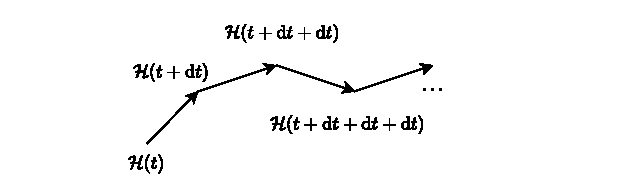
\includegraphics[width=0.6\textwidth]{res/svg/hamiltonian_time_evolution.drawio}
  \caption{Time evolution through Hamiltonian}
\end{figure}
In particular, we can write the Taylor expansion of $u$ and get:
\begin{equation}
  u(t) = u(t_0) + \dv{u}{t}\bigg|_{t_0} (t - t_0) + \frac{1}{2!} \dv[2]{u}{t}\bigg|_{t_0} (t - t_0)^2 + \dots
\end{equation}
We can express the multiple derivatives as:
\begin{equation}
  \begin{split}
    \dv{u}{t} &= \pb{u}{\hamfun}\\
    \dv[2]{u}{t} &= \pb{\pb{u}{\hamfun}}{\hamfun}\\
    \dv[3]{u}{t} &= \pb{\pb{\pb{u}{\hamfun}}{\hamfun}}{\hamfun}\\
    &\dots
  \end{split}
\end{equation}
We then define the operator $\hat{H}$ such that:
\begin{equation}
  \hat{H} = \pb{}{\hamfun}
\end{equation}
And so we can write the Taylor series as:
\begin{equation}
  \begin{split}
    u(t) &= u(t_0) + \hat{H}u(t)\bigg|_{t_0} (t - t_0) + \frac{1}{2!} \hat{H}^2u(t)\bigg|_{t_0} (t - t_0)^2 + \dots =\\
    &= \bigsum_{k=0}^\infty \dfrac{1}{k!} \hat{H}^k u(t)\bigg|_{t_0}(t - t_0)^k =\\
    &= u(t_0)\bigsum_{k=0}^\infty \dfrac{1}{k!} \hat{H}^k (t - t_0)^k \defineeq u(t_0) \efunction^{\brackets{t-t_0}\hat{H}}
  \end{split}
\end{equation}
Keep in mind that the last step is more of a "definition" consistent with the fact that we would get exactly the Taylor series of the exponential if we replaced $\hat{H}$ with a usual variable.
This formula is the classical counterpart of the quantum mechanical "propagator". In particular, we notice that in both cases the formula contains the Hamiltonian (the operator made from the Poisson brackets in the classical case and the operator associated to the Hamiltonian in the quantum case) and also that both are used to get the time evolution of something.


\backmatter

% input{_postamble.tex}
\end{document}
